\chapter{Signal and background modelling}
\label{chap:model}

The statistical interpretation of the data relies on accurate modelling the shape and normalisation of the \mgg distribution for the signal and background processes in each category. %The signal here refers to the diphoton events produced by one of the main Higgs production processes \ggH, \VBF, \ttH, and \VH, where the latter can be further split into \WH and \ZH. 
For the signal processes, this distribution takes the form of a resonant peak around \mH, the width of which is entirely dominated by detector resolution. The construction of the signal model is described in \Sec~\ref{model:sec:signal_model}. By contrast, the invariant mass distribution of background events is a continuously falling non-resonant continuum. The data-driven method by which the background model is produced is described in \Sec~\ref{model:sec:background_model}. Finally, the handling of the systematic uncertainties is described in \Sec~\ref{model:sec:systematics}. 

\section{Signal modelling}
\label{model:sec:signal_model}

\subsection{Parametrisation of the signal \mgg distributions}

The signal model is constructed from samples of simulated \Hgg events from each production mode. The events from the \VH mode are further split into \WH and \ZH samples. % are reconstructed, selected and categorised as described in Chapters~\ref{} and ~\ref{}. 
The shape of the \mgg distribution is parametrised separately for each process in each event category. Since the vertex choice affects the shape of the \mgg  of the distribution, as was mentioned in \Sec~\ref{}, the modelling is done separately for cases where the \RV or \WV  was selected. 

The signal \mgg distributions are all parametrised using a \DCB~\ref{} function with an additional Gaussian function sharing the same mean. This is in contrast with the functional form used in~\cite{HIG-16-020}, which was a sum of up to five Gaussian functions, where the number of functions in th sum was tuned for each \mgg distribution. %The \CB functional form is used in \HEP to model processes which involve losses, for example in the semiparmetric regression described in Sec~\ref{}, where it is used to model the energy of individual photons. 
The \DCB shape consists of a Gaussian function core and two tails which are described by power laws. The Gaussian core represents the intrinsic width of the distribution being modelled, while the tails model the under- or over-estimation of the value of the parameter of interest. %For example, the \DCB shape is used iin the semiparmetric regression described in \Sec~\ref{} to model photon energy distribution. The lower tail captures the fact that a certain amount of energy of the photon can be lost in the reconstruction process, this leading to a long non-Gaussian tail of events. Ont he other side, the upper tailis motivated theenergy of the photon shower can be over-estimated, for example because of the inclsuio of showers due to \PU.  
The \DCB shape has five parameters: the width and mean of the Gaussian core, the cross-over points to the power laws on each side, and the order of the two power laws. The functional \DCBpG form also incorporates an additional Gaussian function, which shares the same mean as the \DCB, leading to a total of seven parameters once the extra Gaussian width and mixing fraction are accounted for. 

The choice of the \DCBpG functional form to parametrise the signal distributions was motivated by the fact that the resulting parametrisation of the signal shape gave closer agreement to the simulated distributions than the simple sum of Gaussian function, but with substantially fewer degrees of freedom. The \DCB shape is also better motivated physically than an arbitrary sum of Gaussian functions. 

The values of the parameters of the functioanl form are determined perfoming a \NLL fit of functional for to the simulated \mgg distrubutions. The resulting parametrisations of the \mgg distributions for the \ggH process (with $\mH=125\GeV$) in the inclusive categories are shown in \Fig~\ref{fig:model:functionalform} for both the \DCBpG and sum of Gaussians functional forms. The improvement in the agreement between the distribution and the parametrisation can be seen by comparing the $\chi^2$ value and the number of degrees of freedom. The \DCBpG always gives a better agreement with a smaller numer of degrees of freedom, and this is also true for the other processes and categories.

\begin{figure}[ht!]
\centering
  \subfloat[Functional form: DCB$+1$G]{\shortstack{
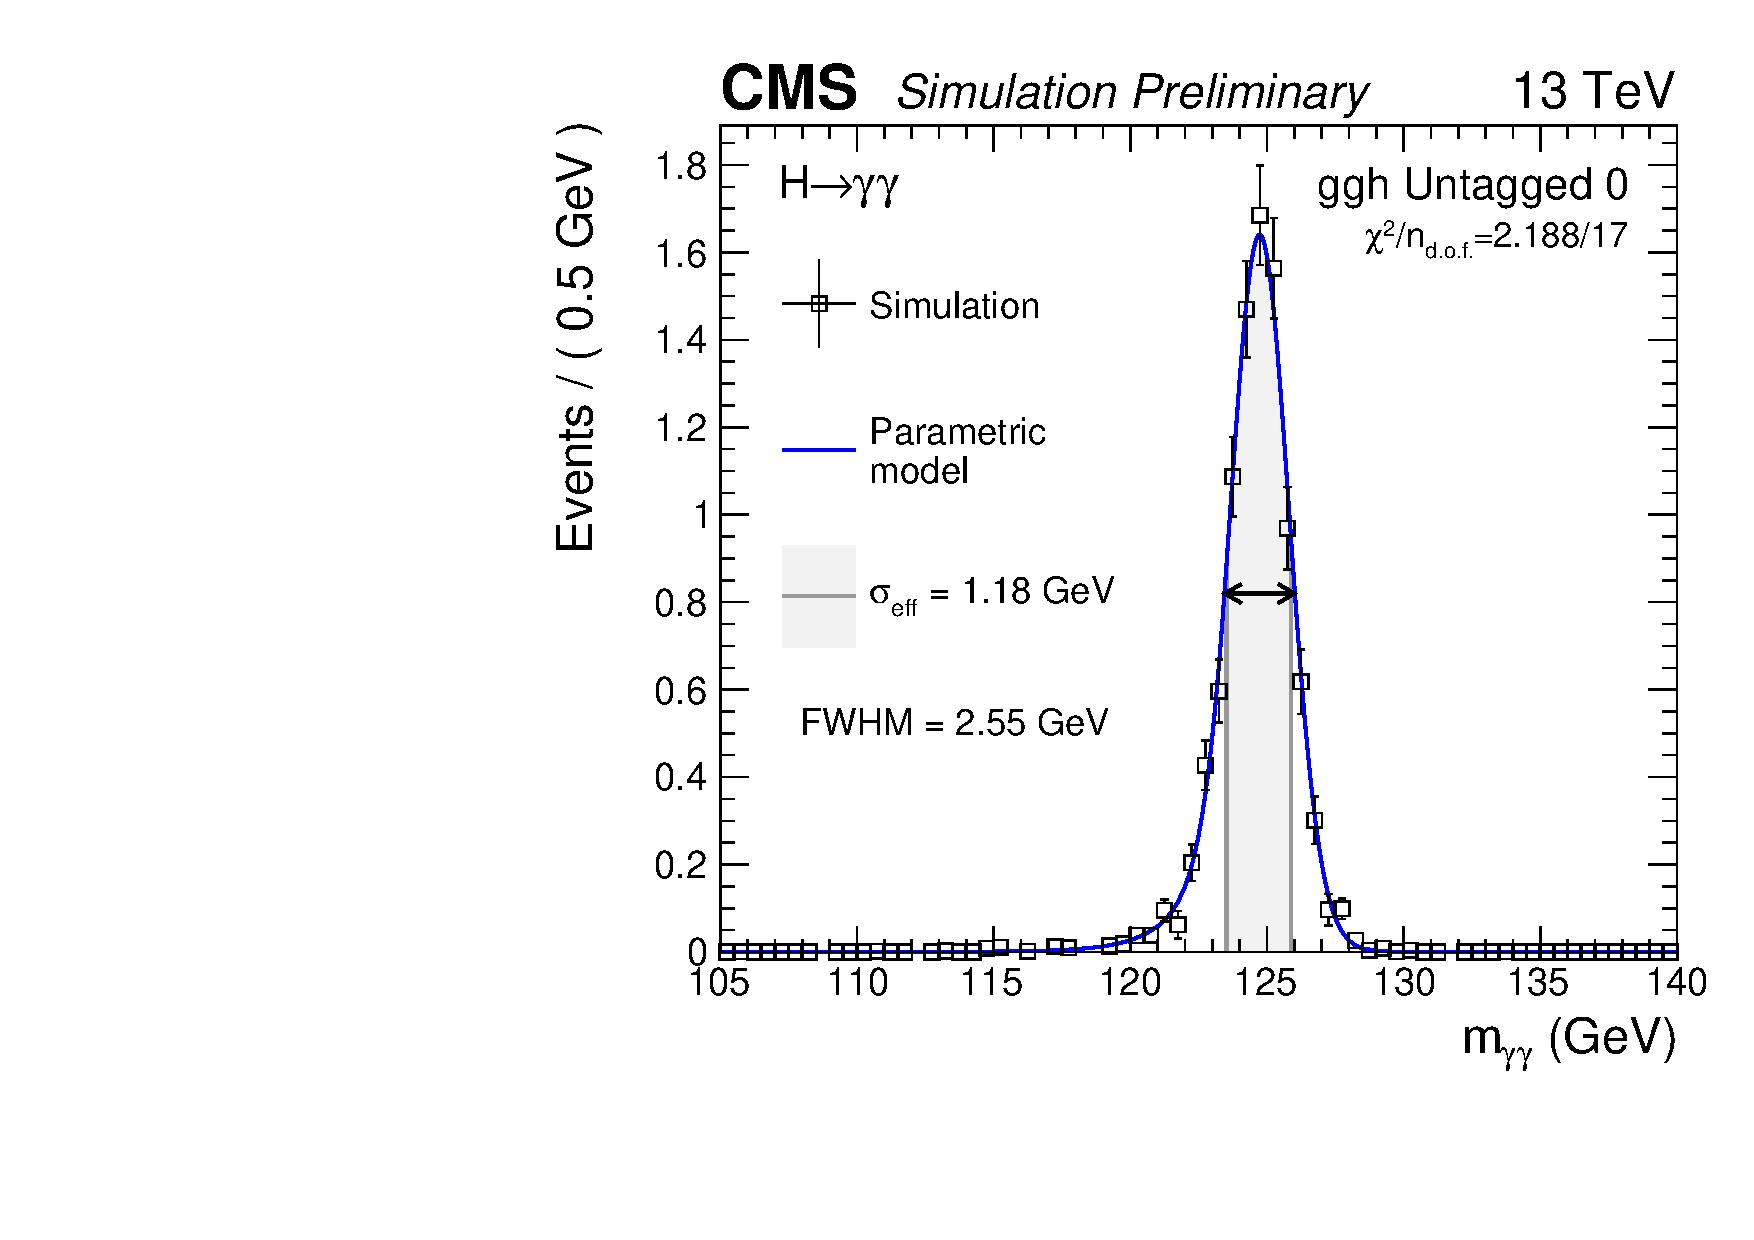
\includegraphics[width=0.3\textwidth]{modellingFigures/DCBpG/ggh_UntaggedTag_0.pdf} 
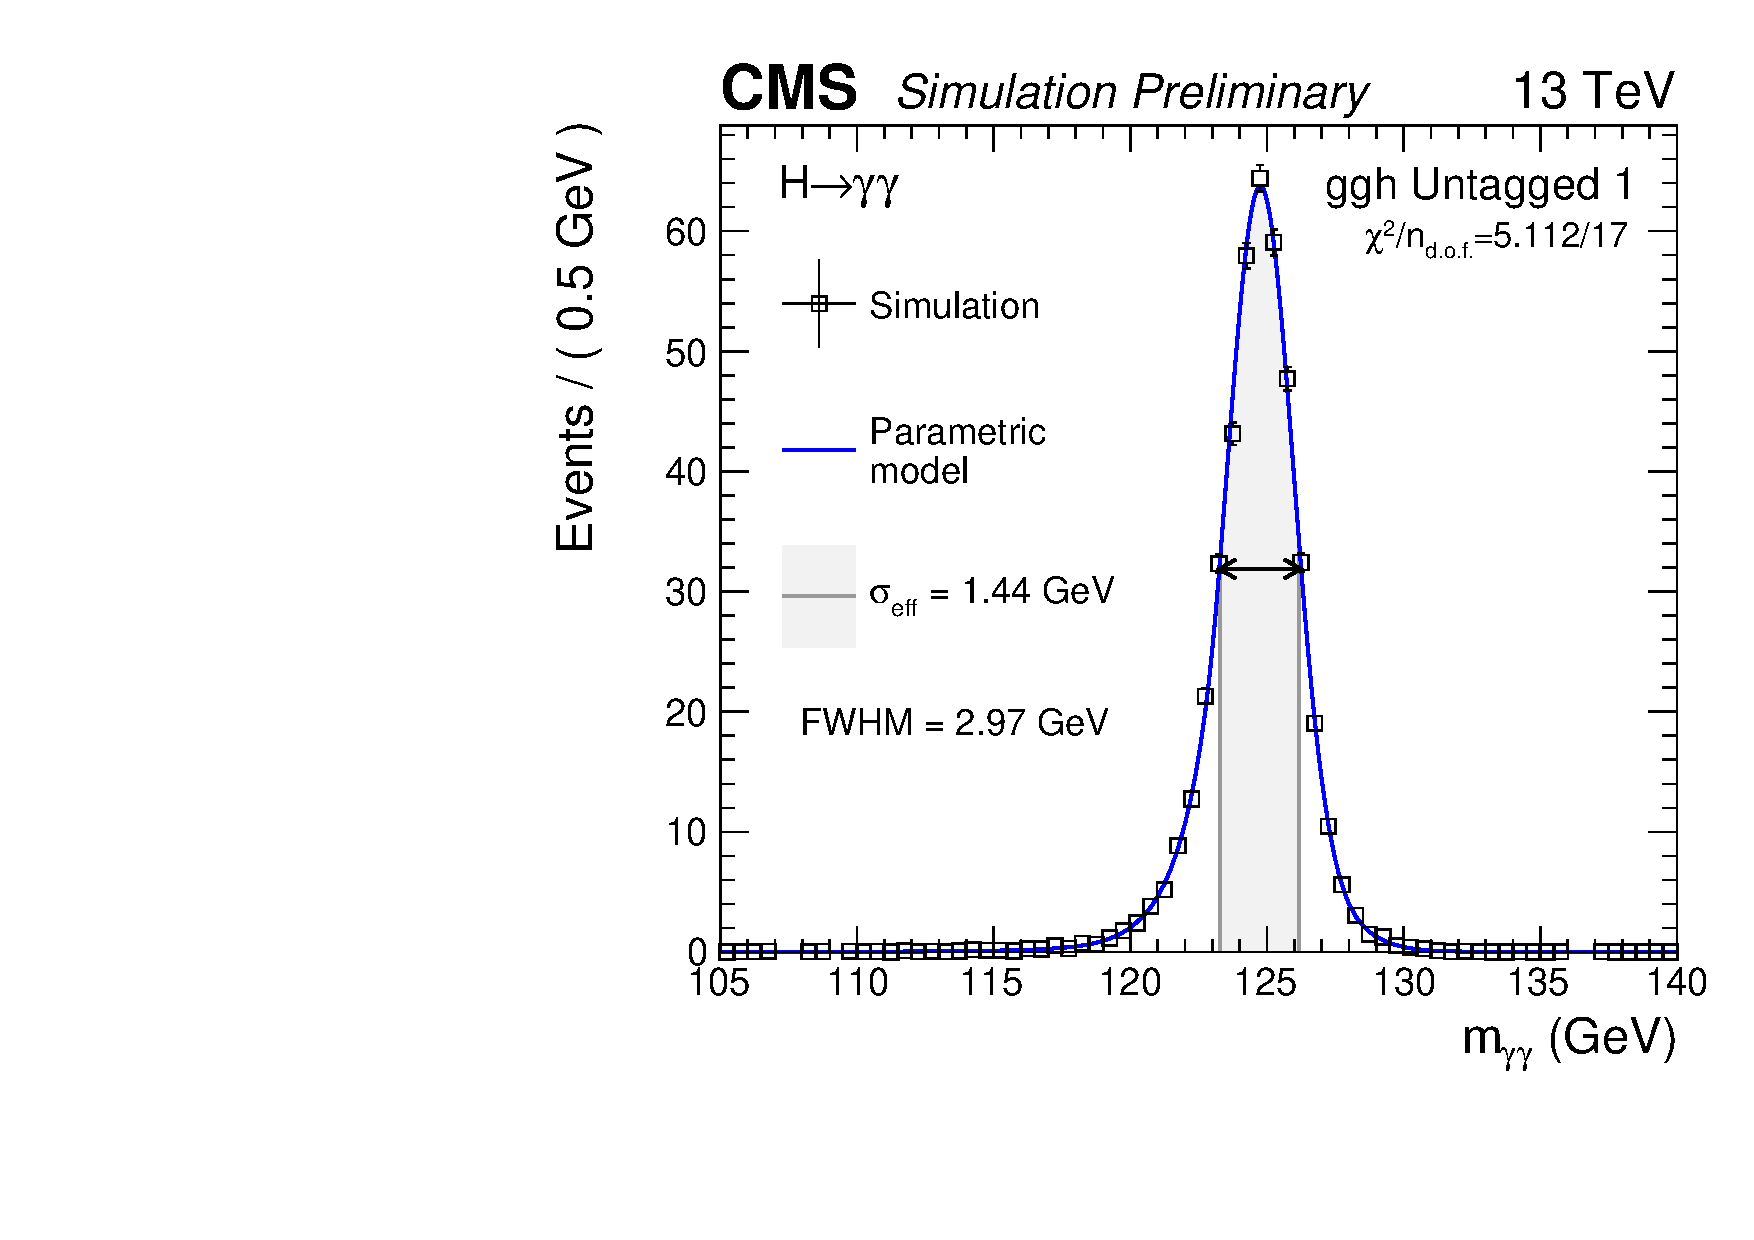
\includegraphics[width=0.3\textwidth]{modellingFigures/DCBpG/ggh_UntaggedTag_1.pdf} \\
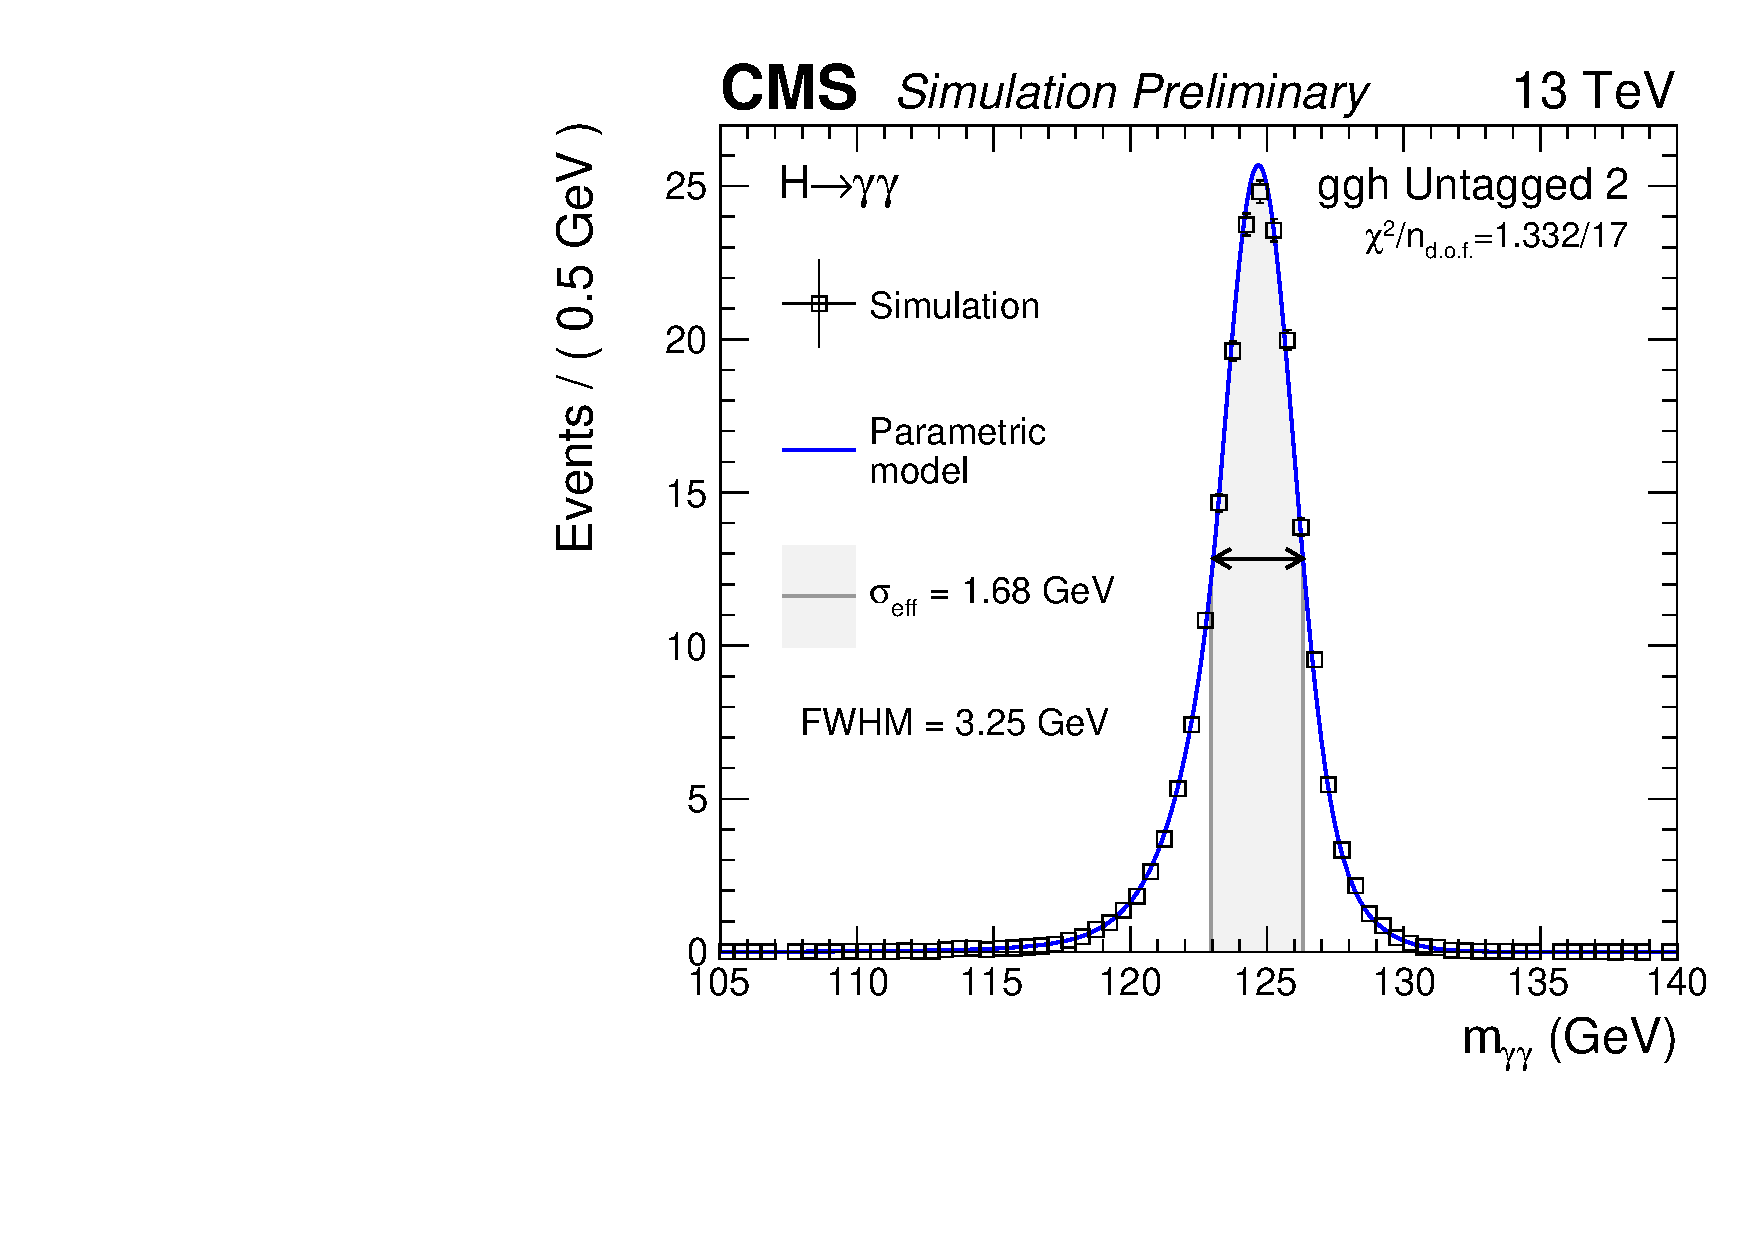
\includegraphics[width=0.3\textwidth]{modellingFigures/DCBpG/ggh_UntaggedTag_2.pdf} 
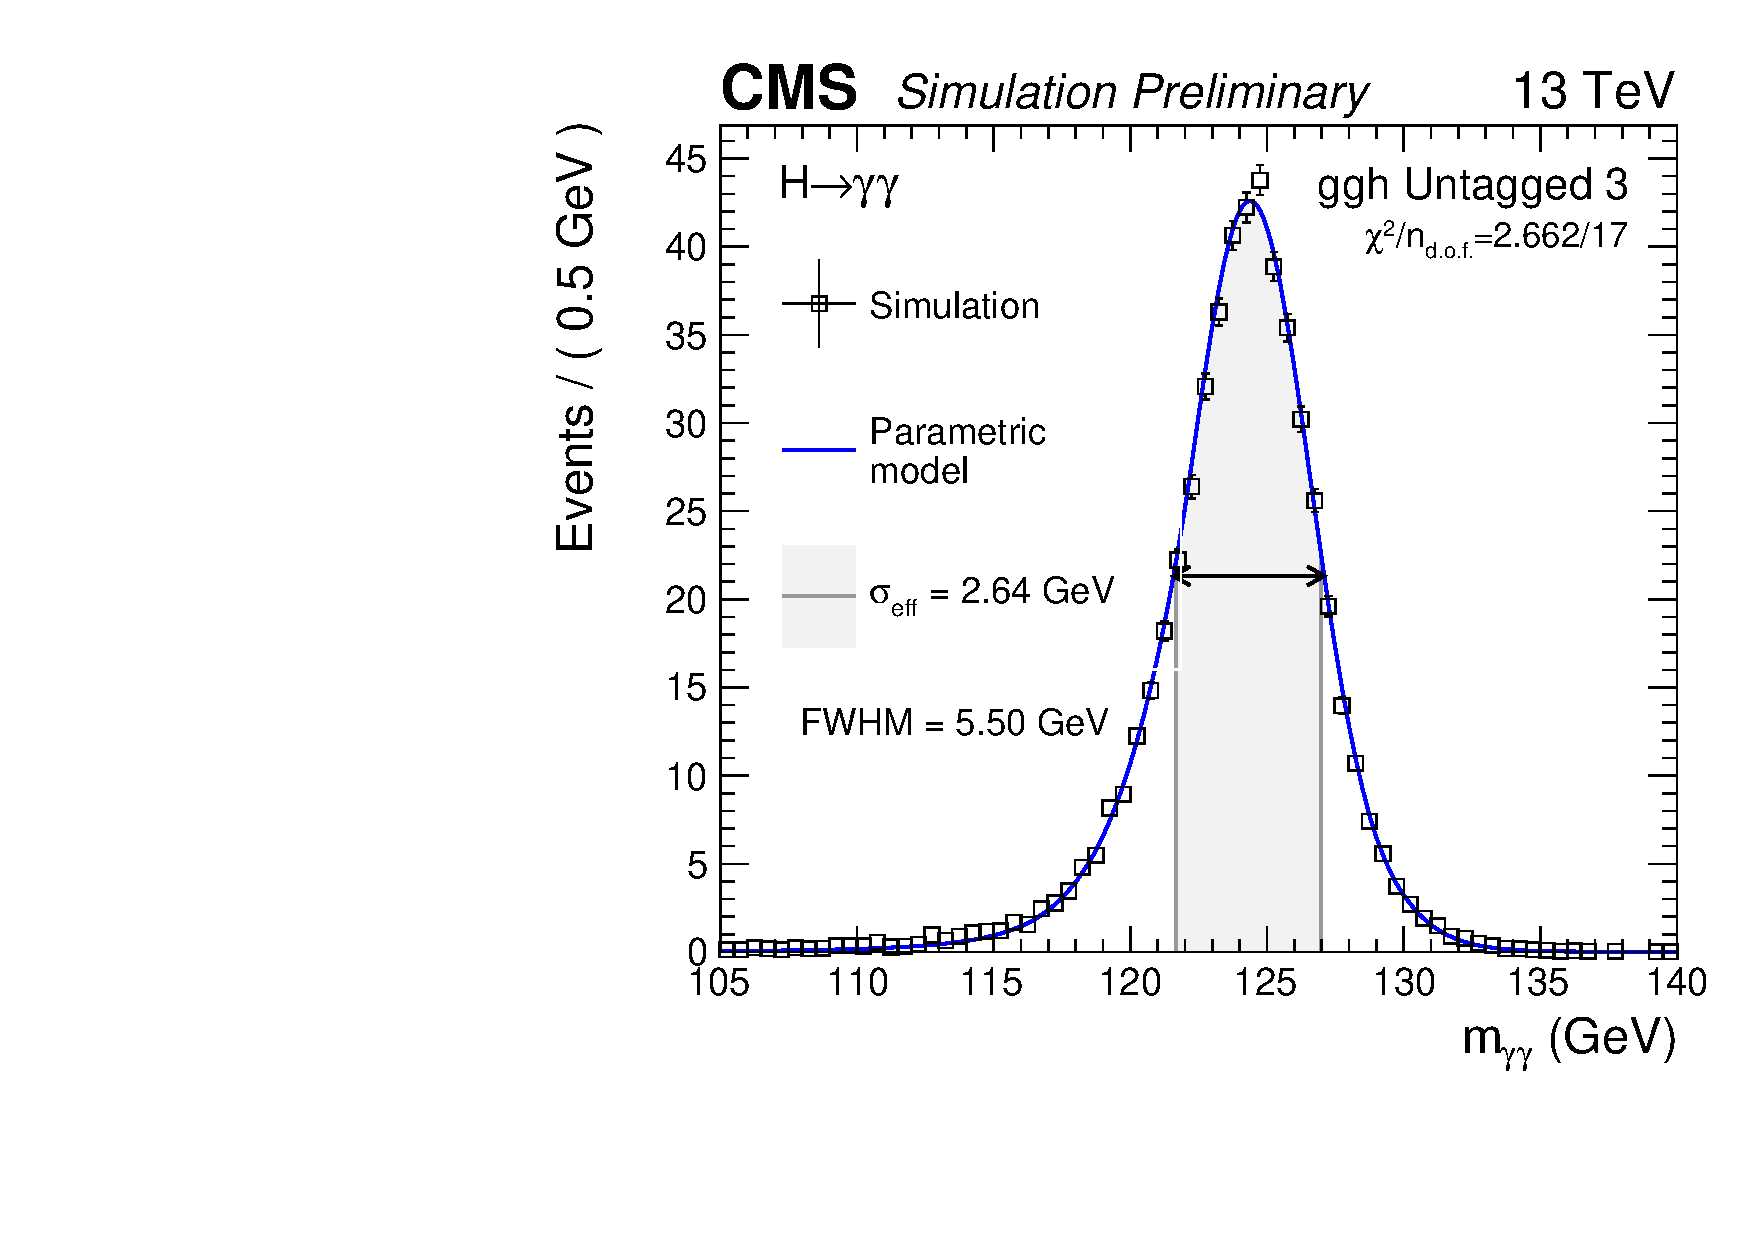
\includegraphics[width=0.3\textwidth]{modellingFigures/DCBpG/ggh_UntaggedTag_3.pdf} 
}}\\
  \subfloat[Functional form: Sum of Gaussians]{\shortstack{
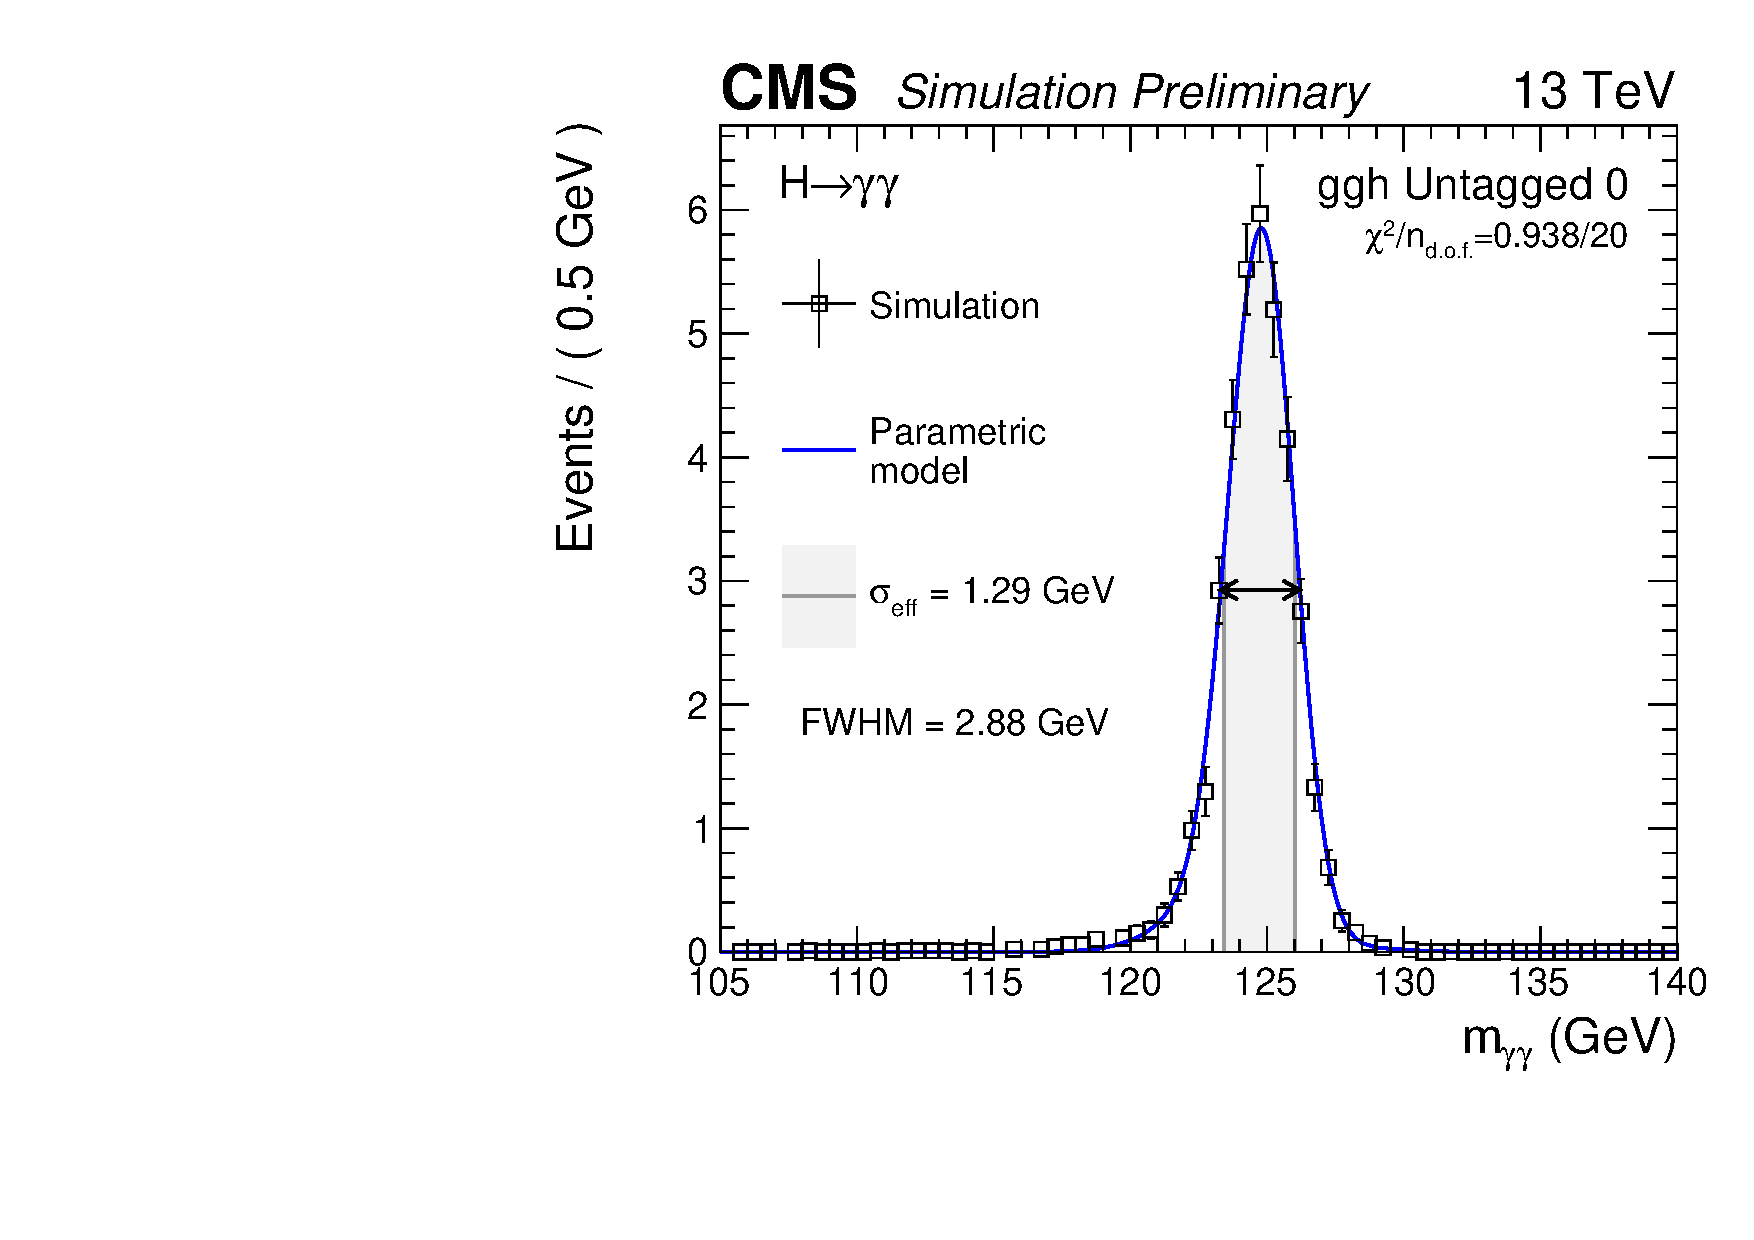
\includegraphics[width=0.3\textwidth]{modellingFigures/nGaus/ggh_UntaggedTag_0.pdf} 
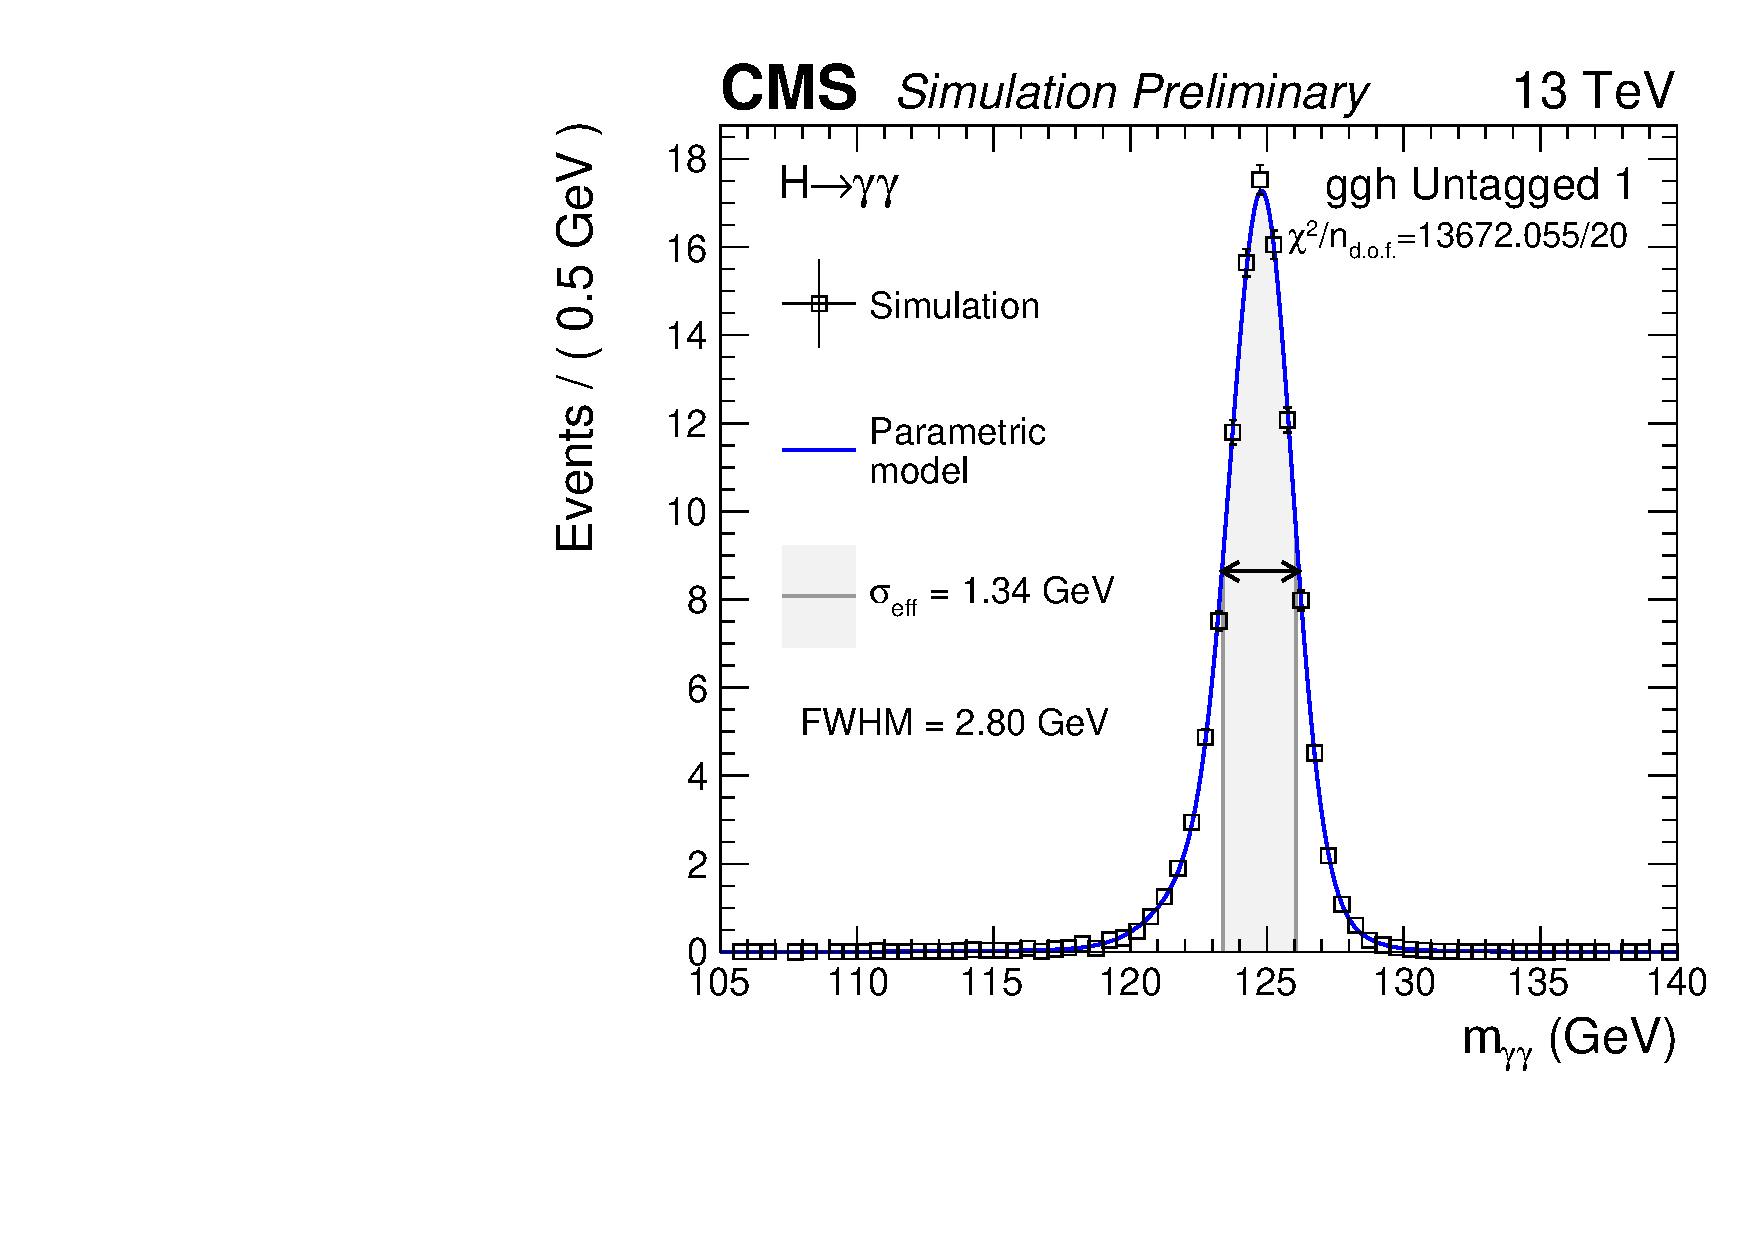
\includegraphics[width=0.3\textwidth]{modellingFigures/nGaus/ggh_UntaggedTag_1.pdf}\\  
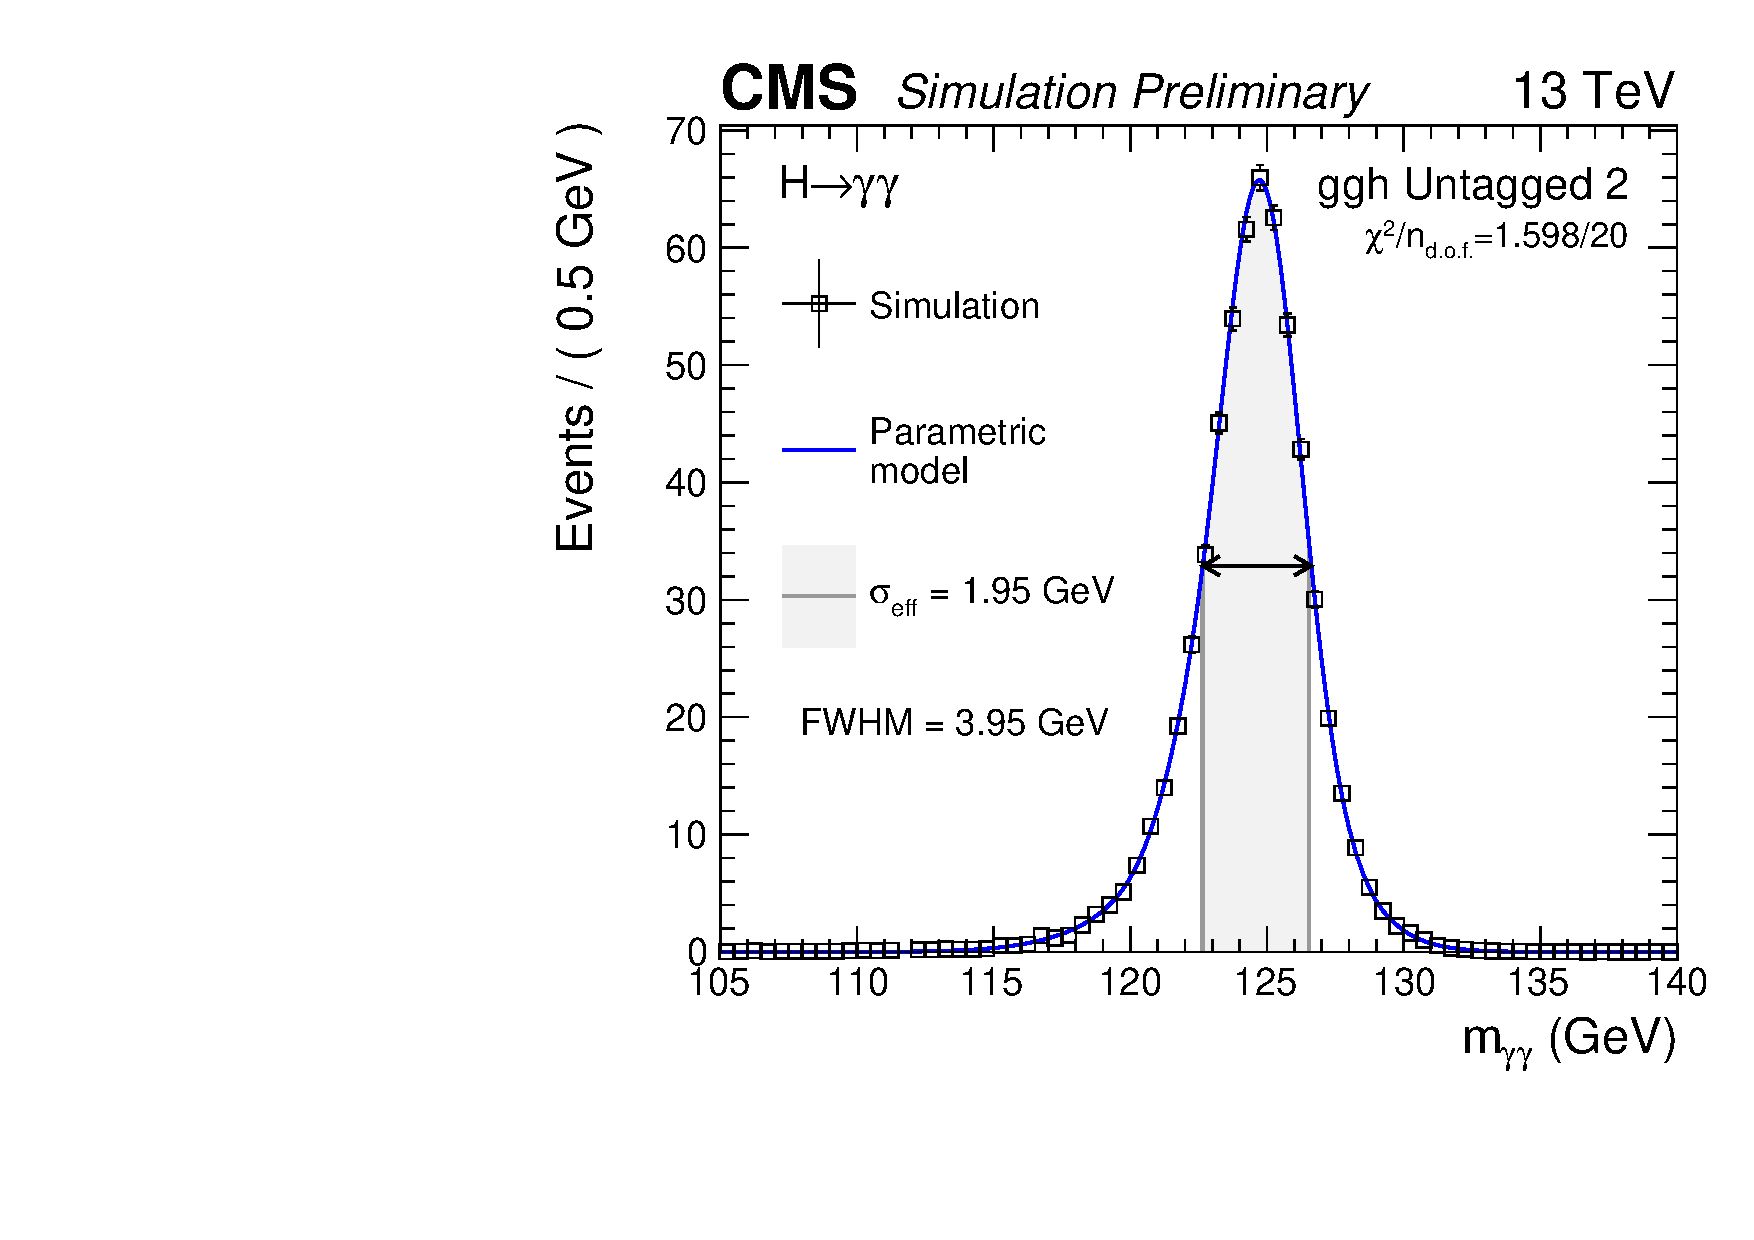
\includegraphics[width=0.3\textwidth]{modellingFigures/nGaus/ggh_UntaggedTag_2.pdf} 
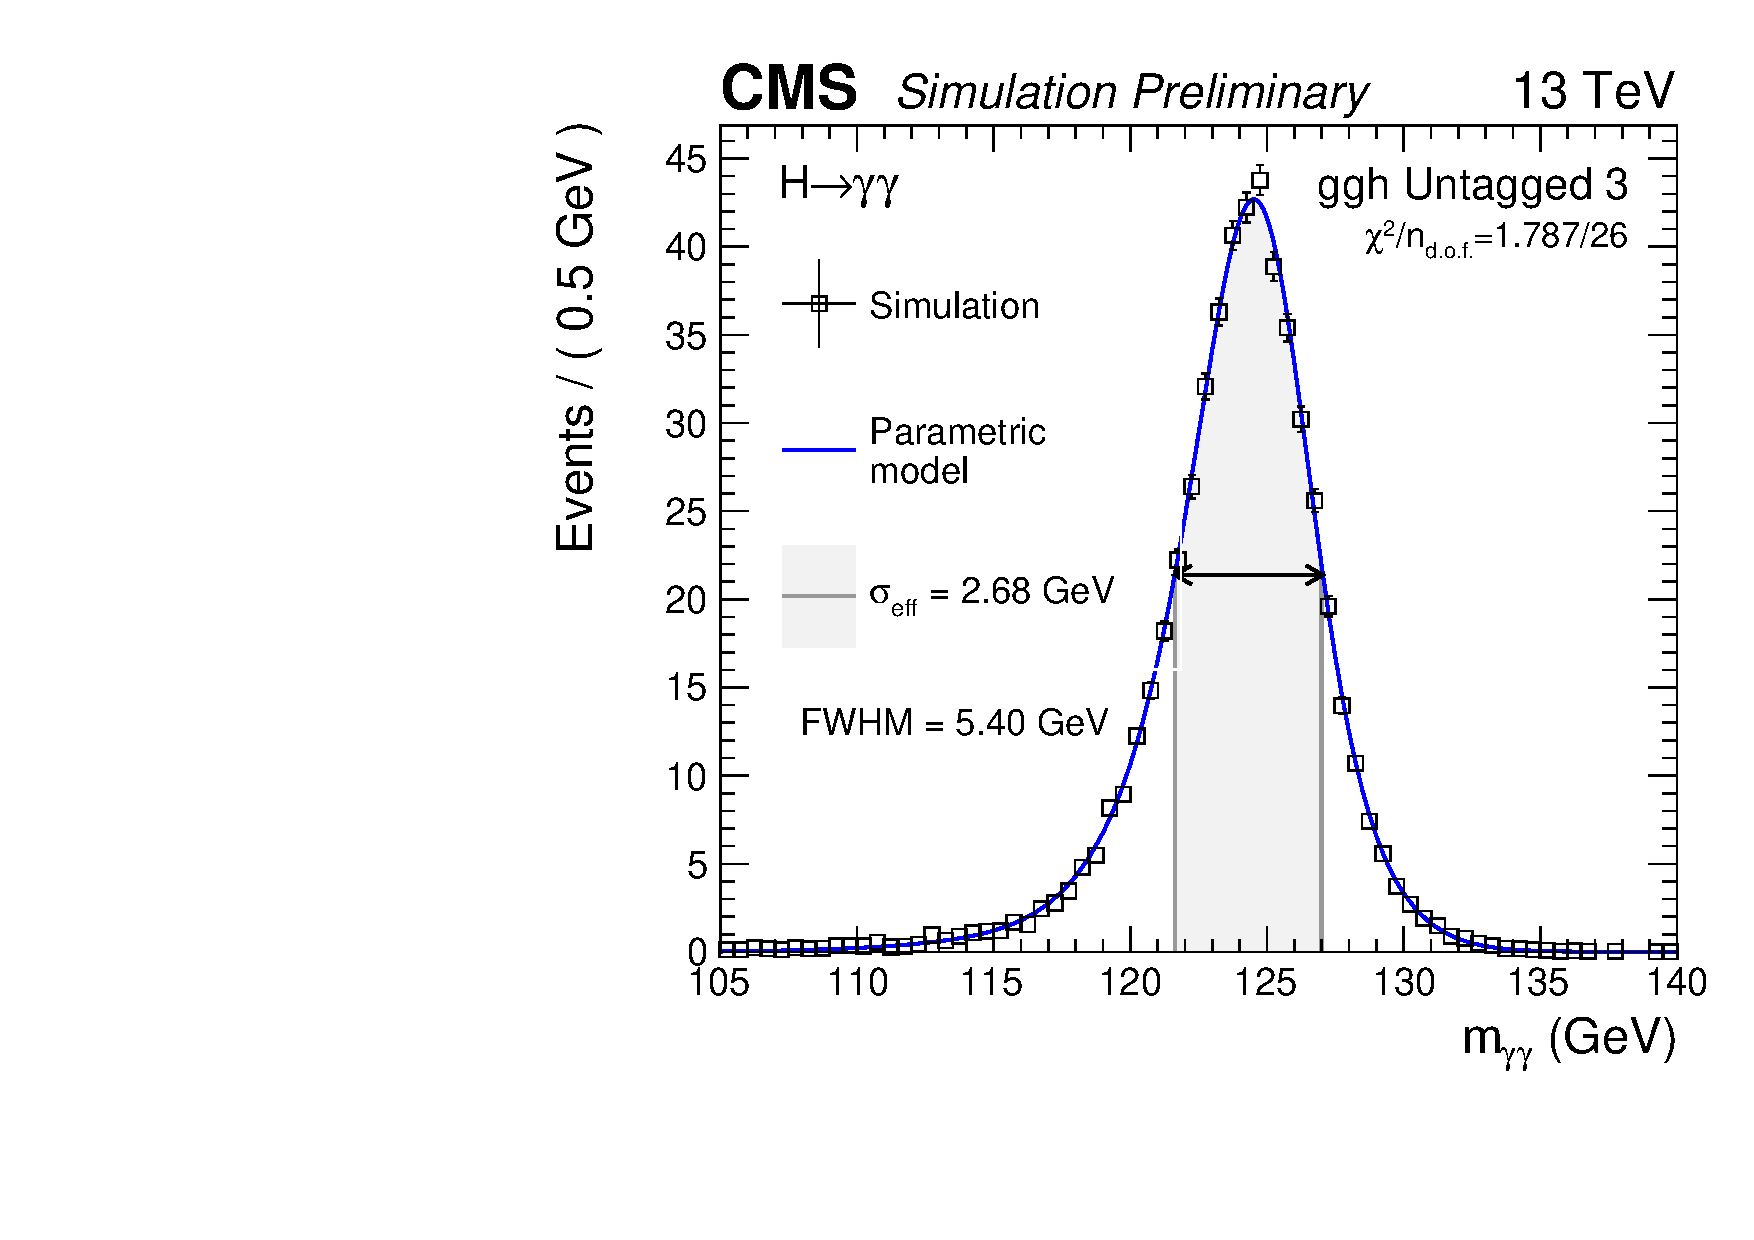
\includegraphics[width=0.3\textwidth]{modellingFigures/nGaus/ggh_UntaggedTag_3.pdf} 
}}
\caption{The shape of the simulated \mgg distribution (\mH=125\GeV) for the \ggH process for the inclusive categories when parametrised with (a) \DCBpG and (b) a sum of Gaussian functions, where the RV and WV contributions have been summed according to their relatove fraction. The plots show the agreement between the simulation and the parametrisation expressed as the $\chi^2$, alongside the total number of degrees of freedom in the parametrisation.}

\label{fig:model:functionalform}
\end{figure}

%A number of checks were performed to validate the use of the \DCBpG shape
%insert tests of different functional forms / appendix ?
%tests on DCB response to signal systematics / appendix ?
%bias studies involving DCB shape / appendix ?
%If the number of events in the sample after splitting into provess, category adn \RV/WV case is too low, it can be extremnely difficult to meaningully fit the \DCB1G shape. In this case, a replacement shape from a related high-statistics category is used to model this tag/process.

\subsection{Dependence of model on \mH}

Since the mass of the Higgs boson is a parameter of interest, the parametrisations from simulated signal samples under different assumptions of the Higgs boson mass are combined to form a single continuous model.  
One option is to perform the fitting procedure described above for each different set of \mH scenarios. The individual parameters of the functional form can then be linearly interpolated from one \mH scenario to the next. This is the approach taken in~\cite{}.

Another option, which is used in this analysis, instead performs a simultaneous fit of all the different \mH samples, where the individual parameters of the functional form are themselves polynomials \mH. The fitting procedure can then occur for all mass scenarios at once, where the floating parameters of the fit are the coefficients of polynomial form of each parameter of the functional form. The advantage of this method, which is called \SSF, is a reduction in the total number of parameters used to determine the full model. Indeed, in the linear interpolation method, the total number of floating parameters is increased for sample with a new \mH, since it is parameterised separately from the others. In the \SSF method the additional degrees of freedom come only from the chosen order of the polynomial describing the parameters in the main functional form). Furthermore, the \SSF method guarantees a sensible continuous model, where the linear interpolation method can lead to discontinuous or unphysical models. 

The \SSF method in this analysis used the \DCBpG functional form and was applied separately for each process, category and \RV/\WV case, using the \mgg distributions from under seven different \mH scenarios: 120, 123, 124,125, 126, 127 and 130\GeV. The \mgg distributions were first normalised to the same event yield. The \SSF method  was tested with the parameters of the functional form cast as polynomials of order 0, 1 and 2. It was found that there was no substantial improvement in the agreement between the model and the \mgg distributions when using polynomials of order greater than 0. This was determined to be because the floating parameters were not sufficiently constrained by the \mgg distributions to bring any meaningful improvement.

The signal models for the \RV and \WV contributions are combined according to their relative fraction. The fraction of events where the selected vertex was within $1\cm$ in the $z$-direction from the true vertex is evaluated for each \mH sample, and then parametrised as a first order polynomial to get a smoth dependence on \mH. 

As an example, the depence on \mH of the signal model for the \ggH process in each of the analysis categories is shown in \Fig~\ref{}. 

\begin{figure}[ht!]
\centering
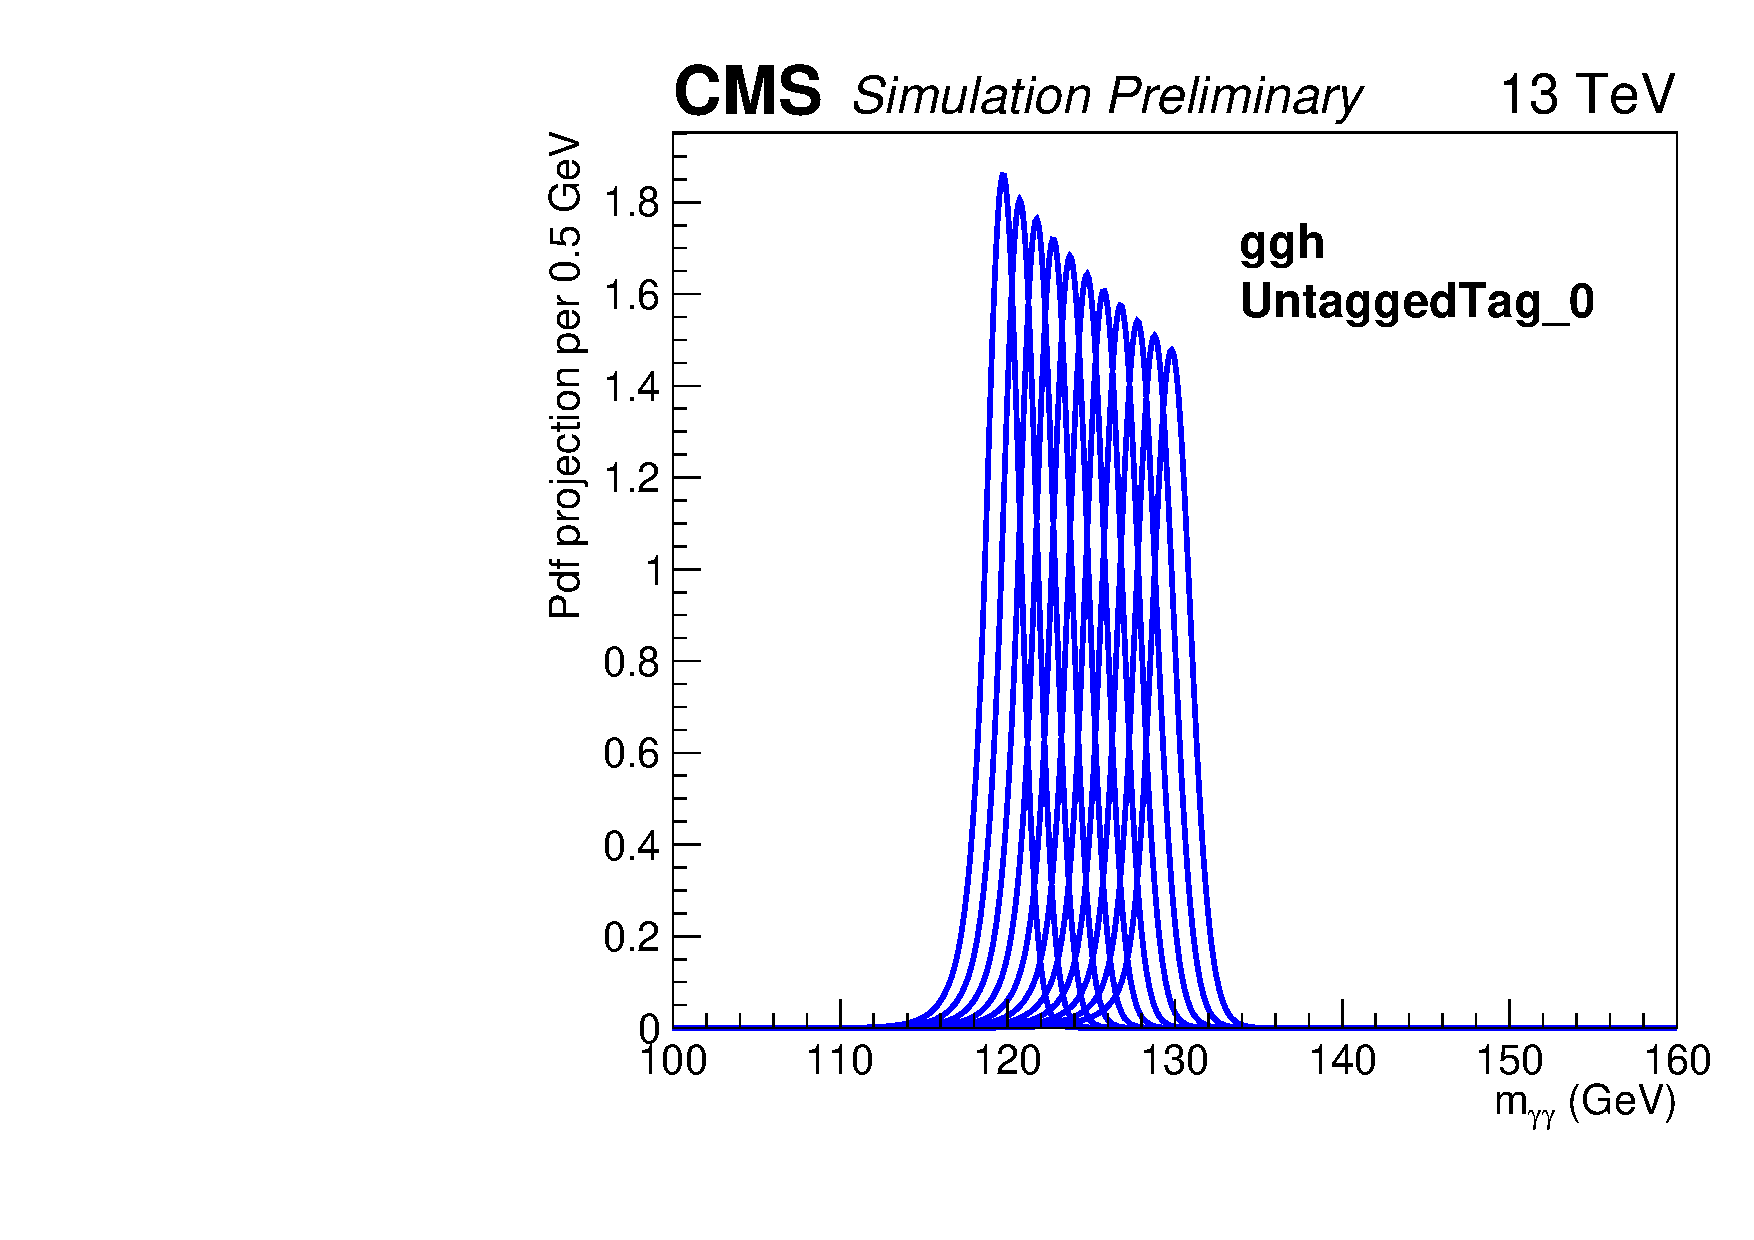
\includegraphics[width=0.3\textwidth]{modellingFigures/DCBpG/ggh_UntaggedTag_0_fmc_interp.pdf} 
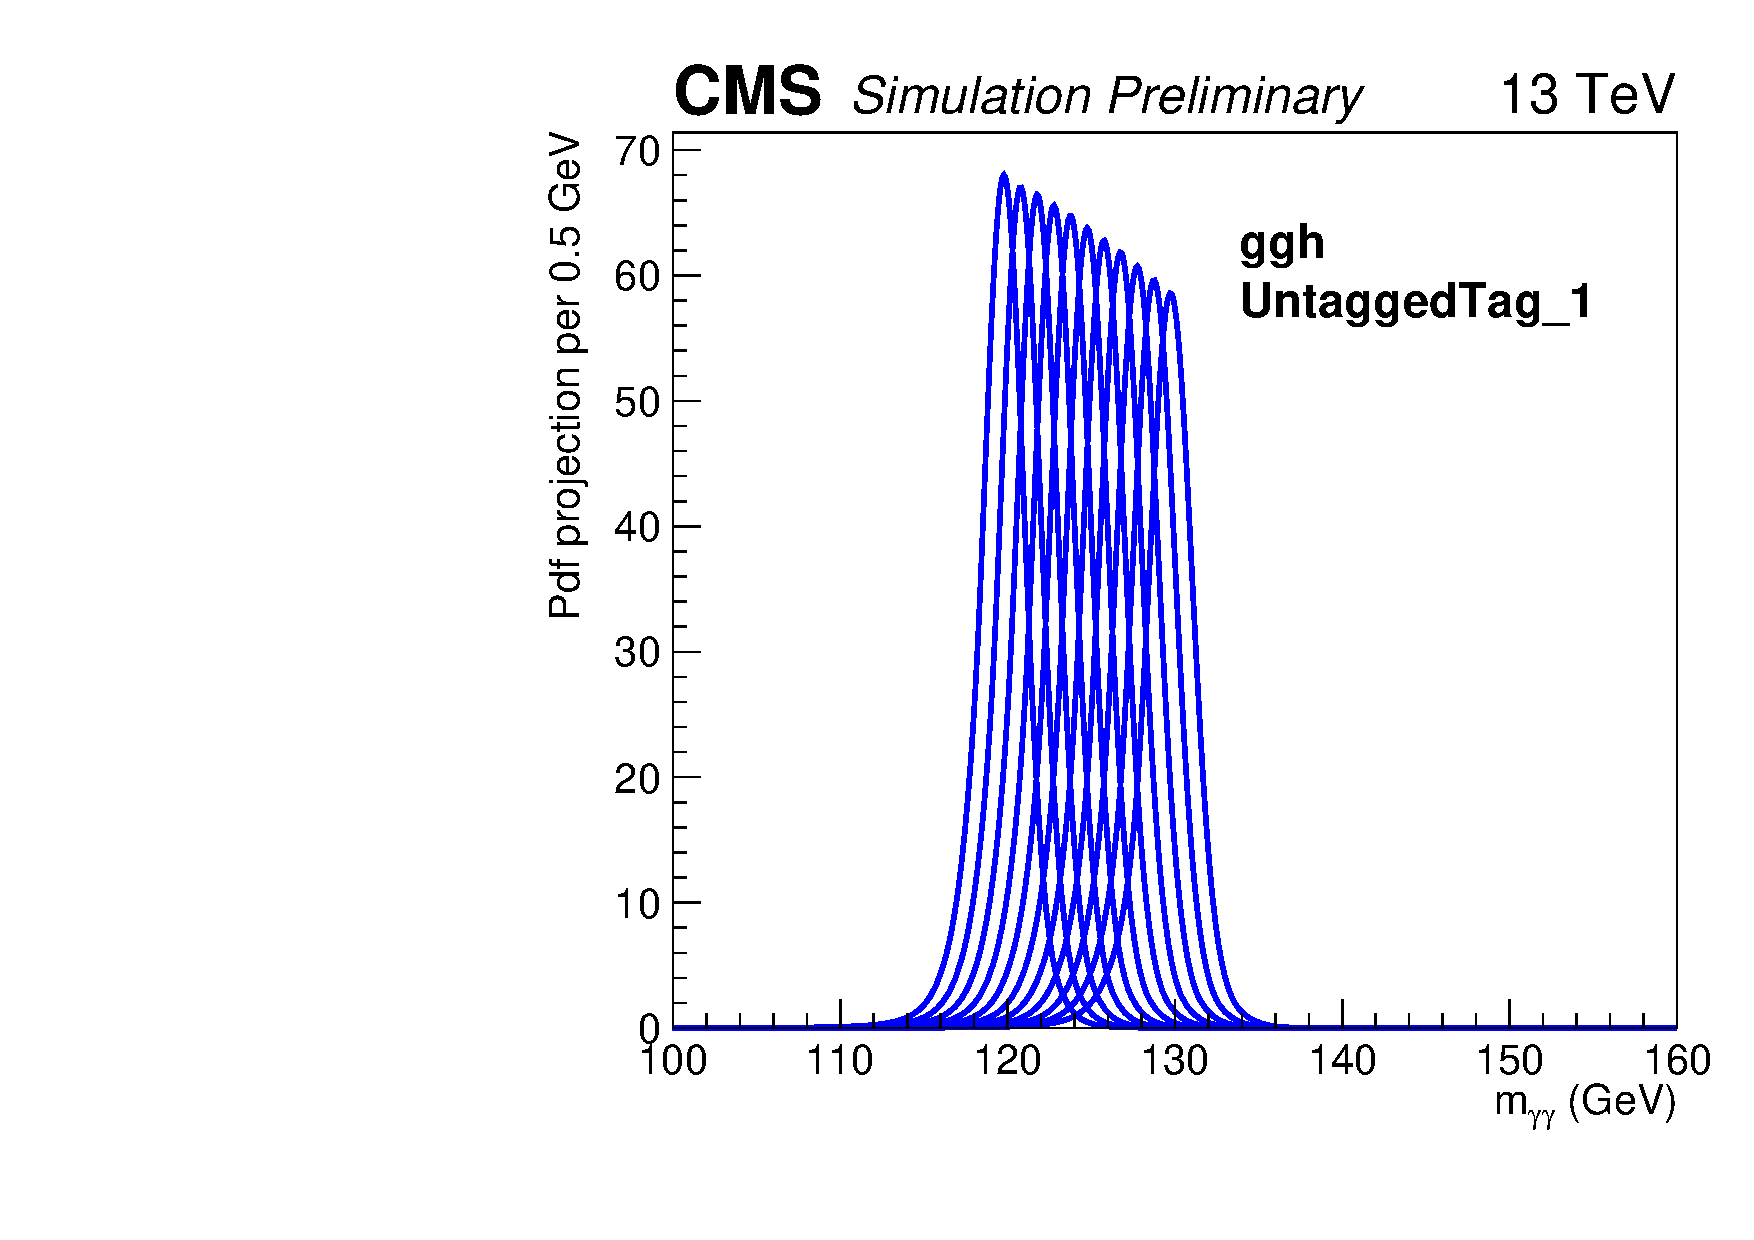
\includegraphics[width=0.3\textwidth]{modellingFigures/DCBpG/ggh_UntaggedTag_1_fmc_interp.pdf} \\ 
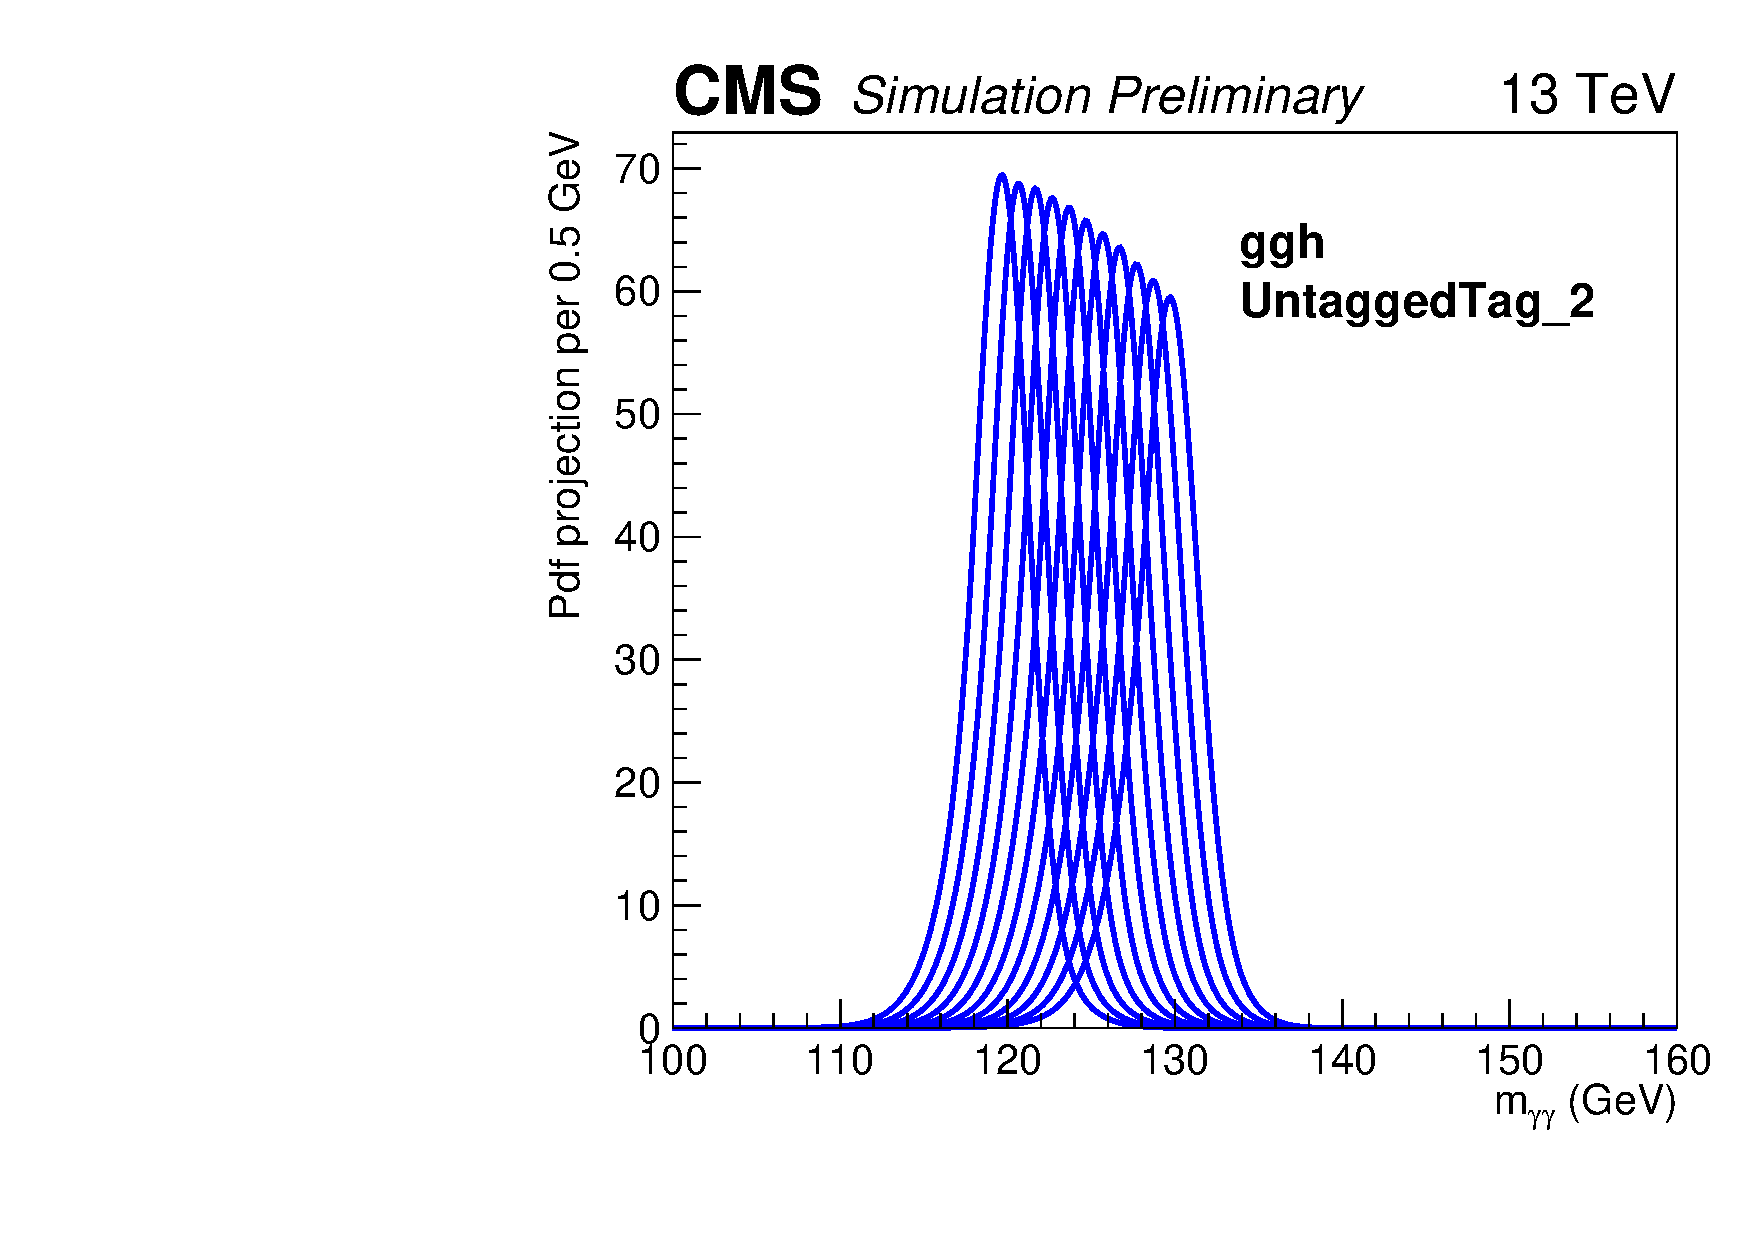
\includegraphics[width=0.3\textwidth]{modellingFigures/DCBpG/ggh_UntaggedTag_2_fmc_interp.pdf} 
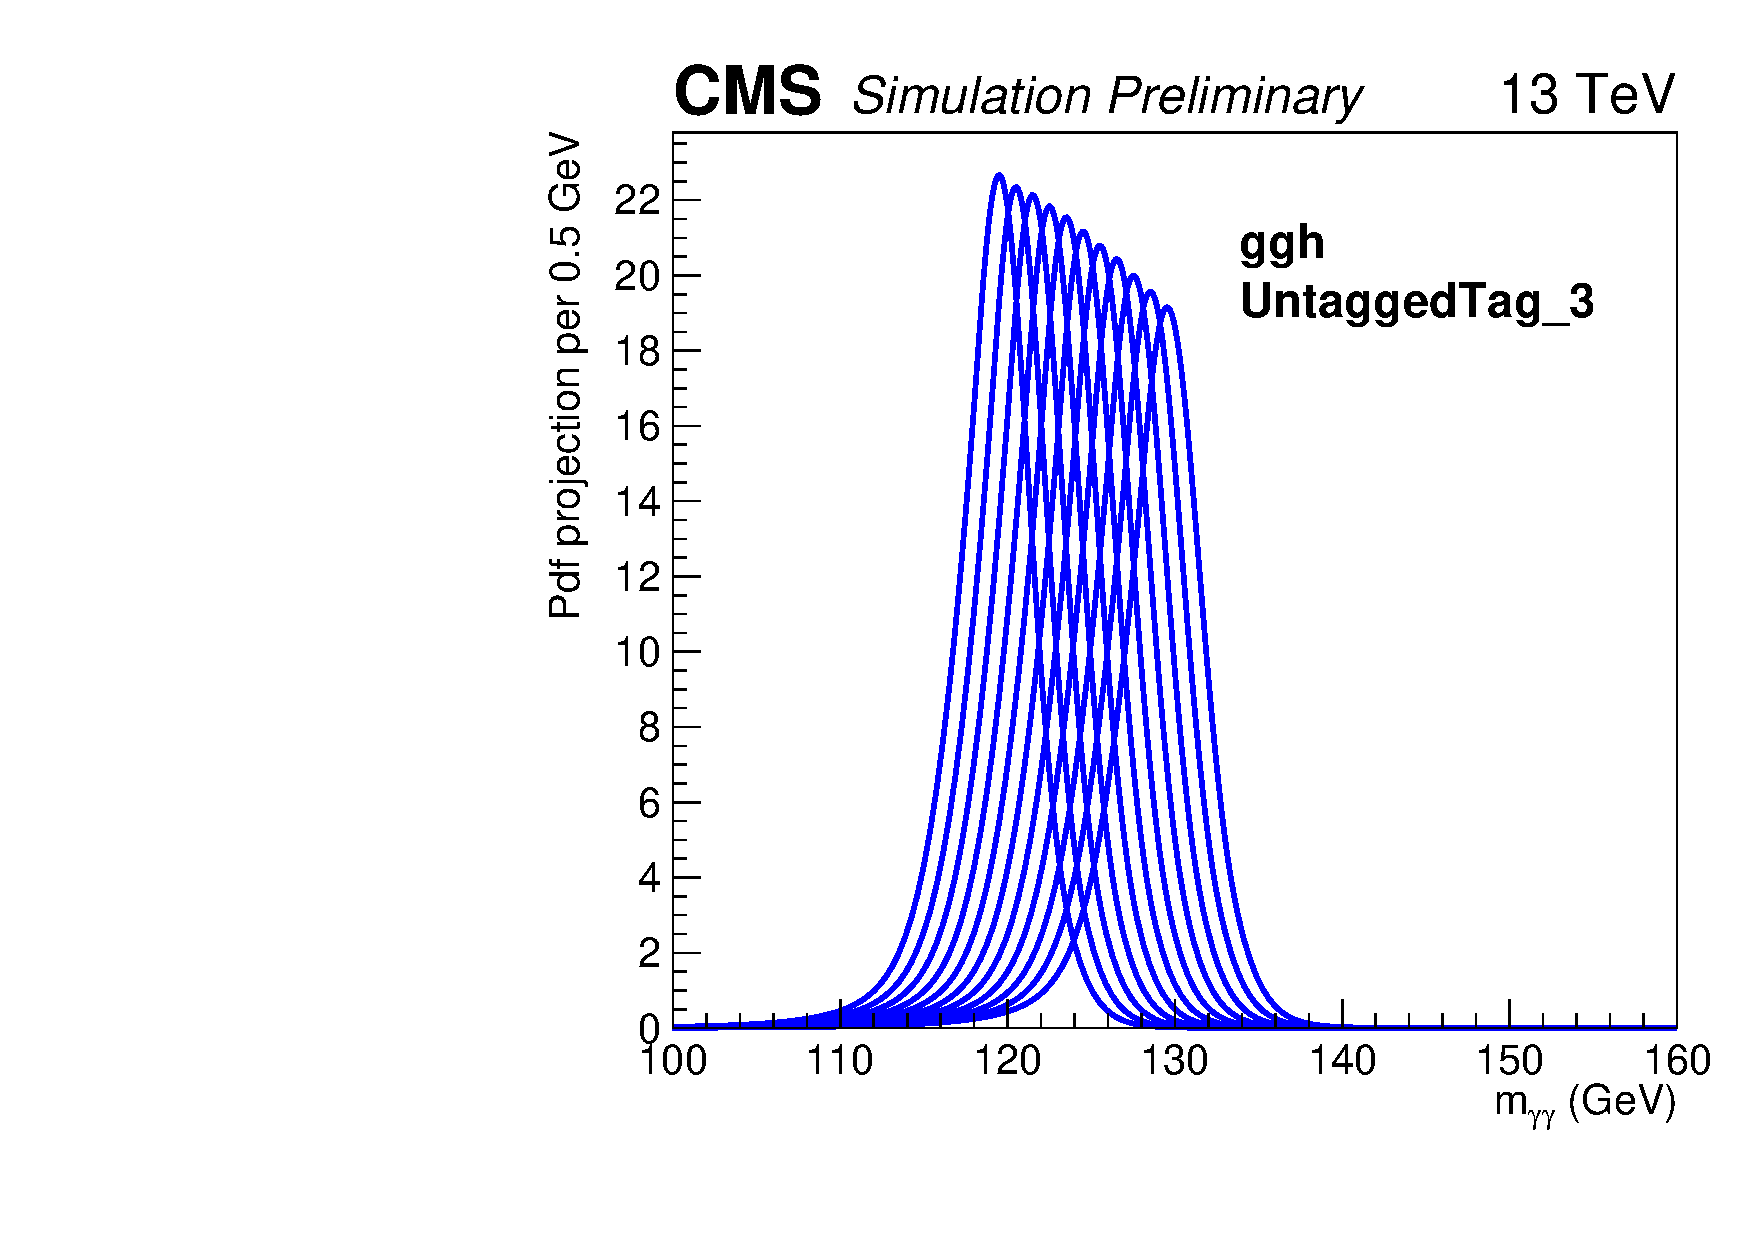
\includegraphics[width=0.3\textwidth]{modellingFigures/DCBpG/ggh_UntaggedTag_3_fmc_interp.pdf} \\
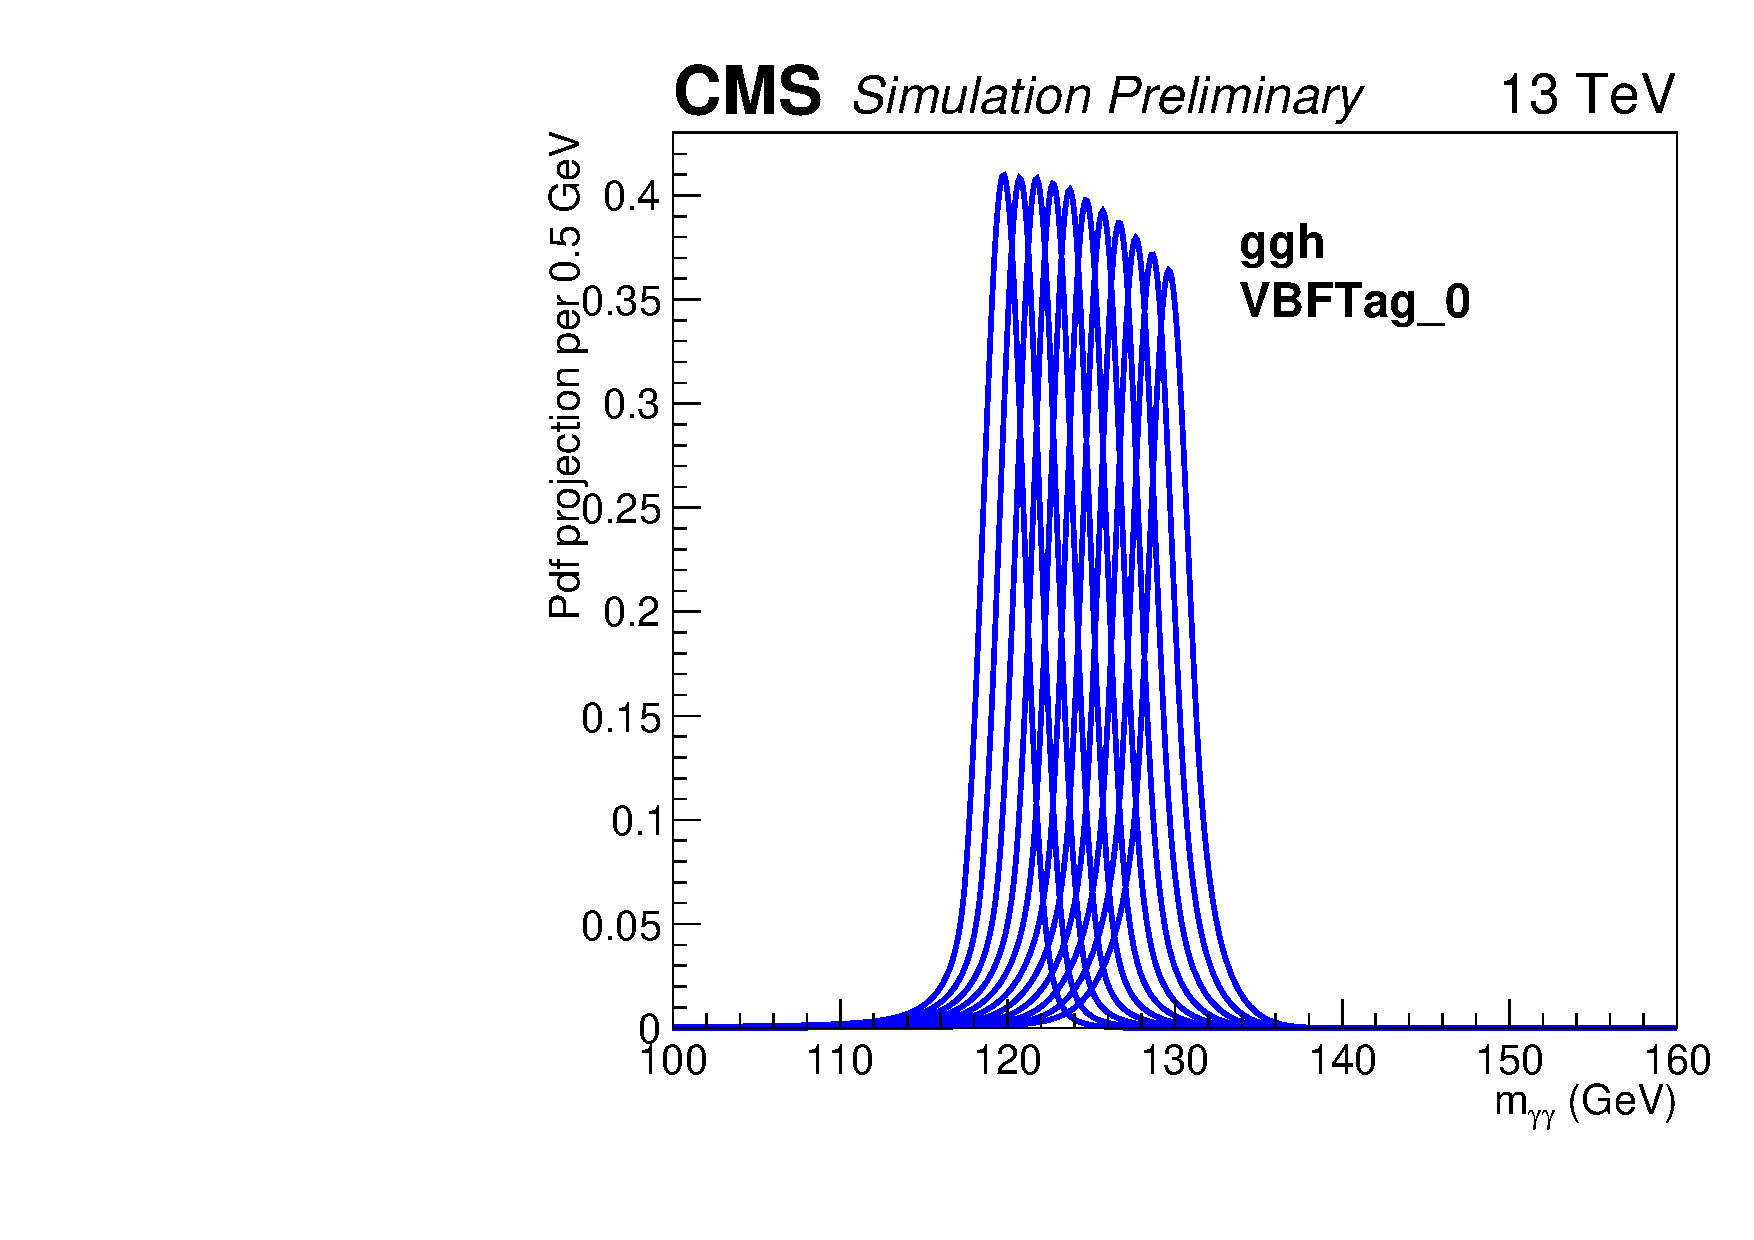
\includegraphics[width=0.3\textwidth]{modellingFigures/DCBpG/ggh_VBFTag_0_fmc_interp.pdf} 
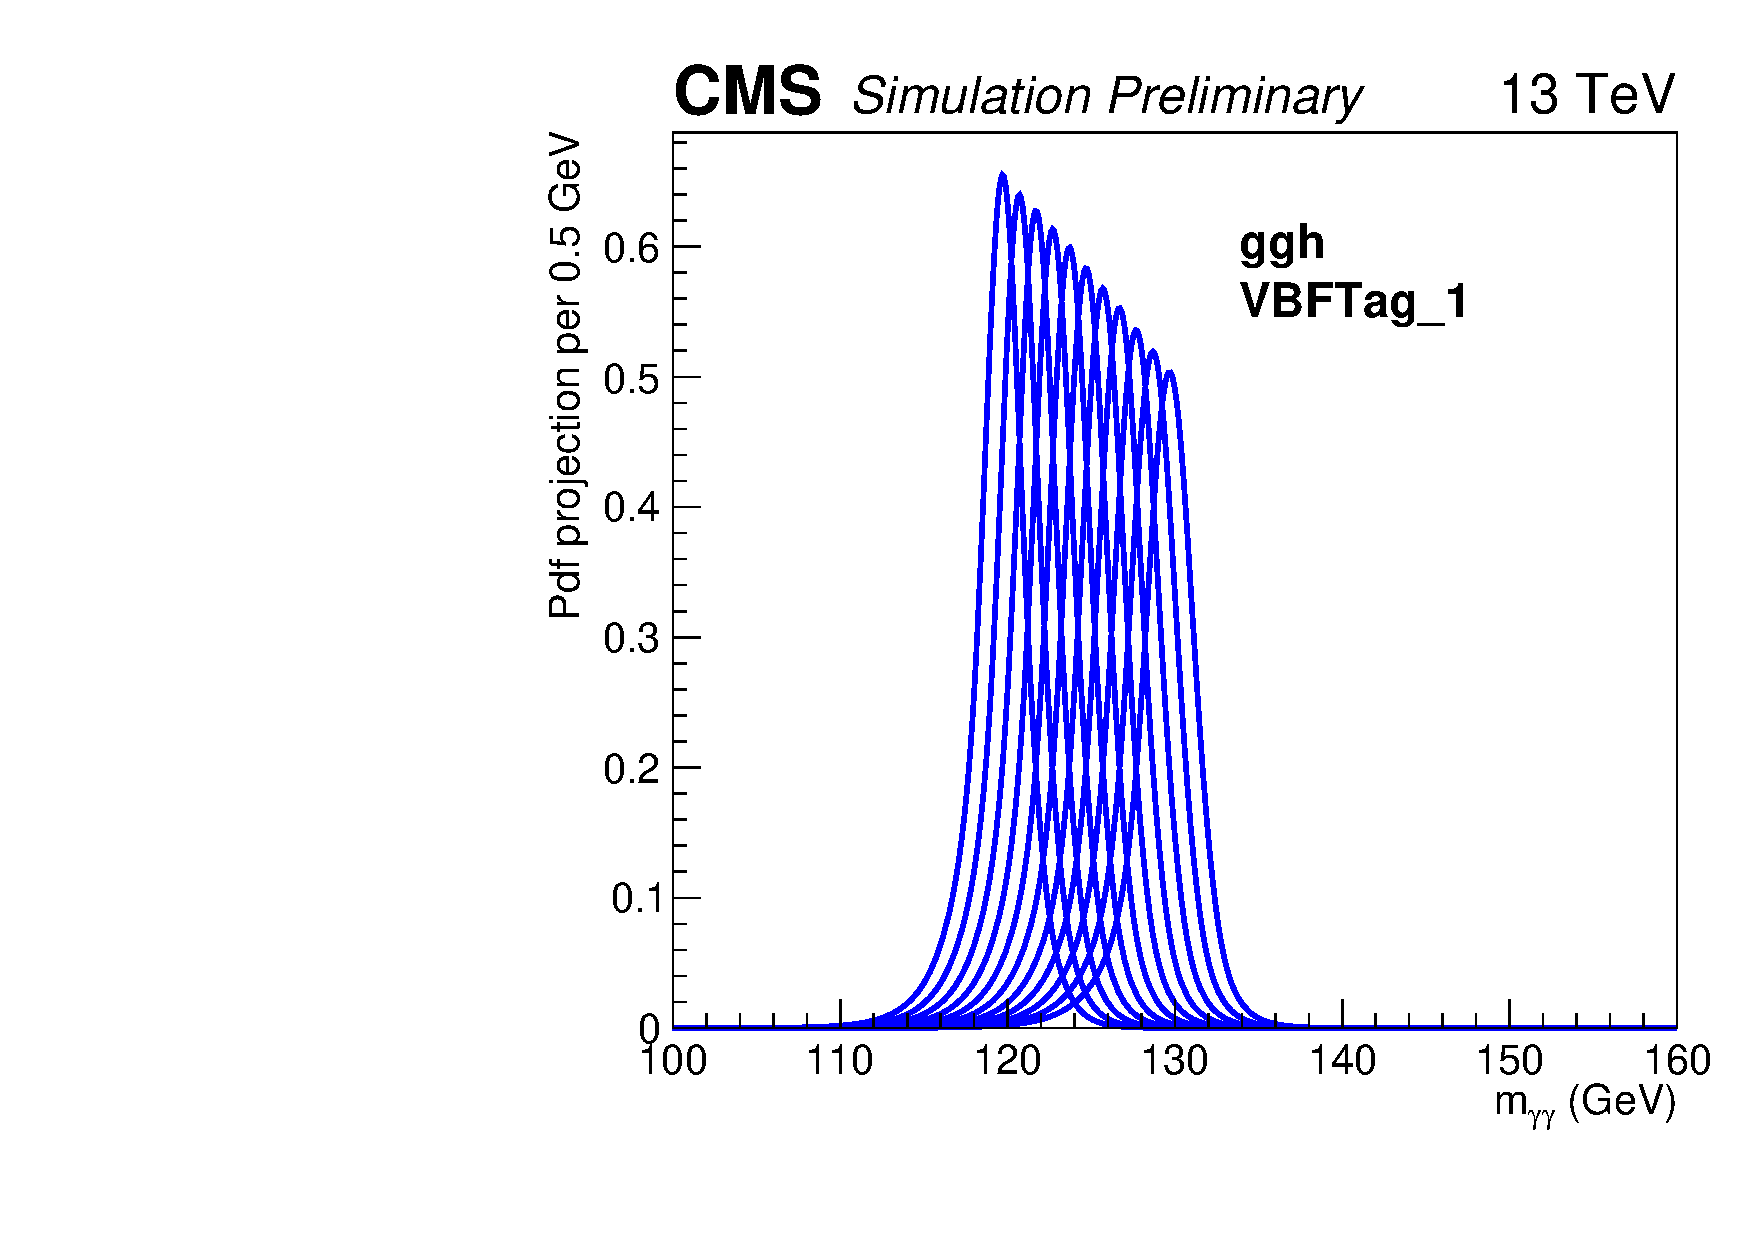
\includegraphics[width=0.3\textwidth]{modellingFigures/DCBpG/ggh_VBFTag_1_fmc_interp.pdf} \\
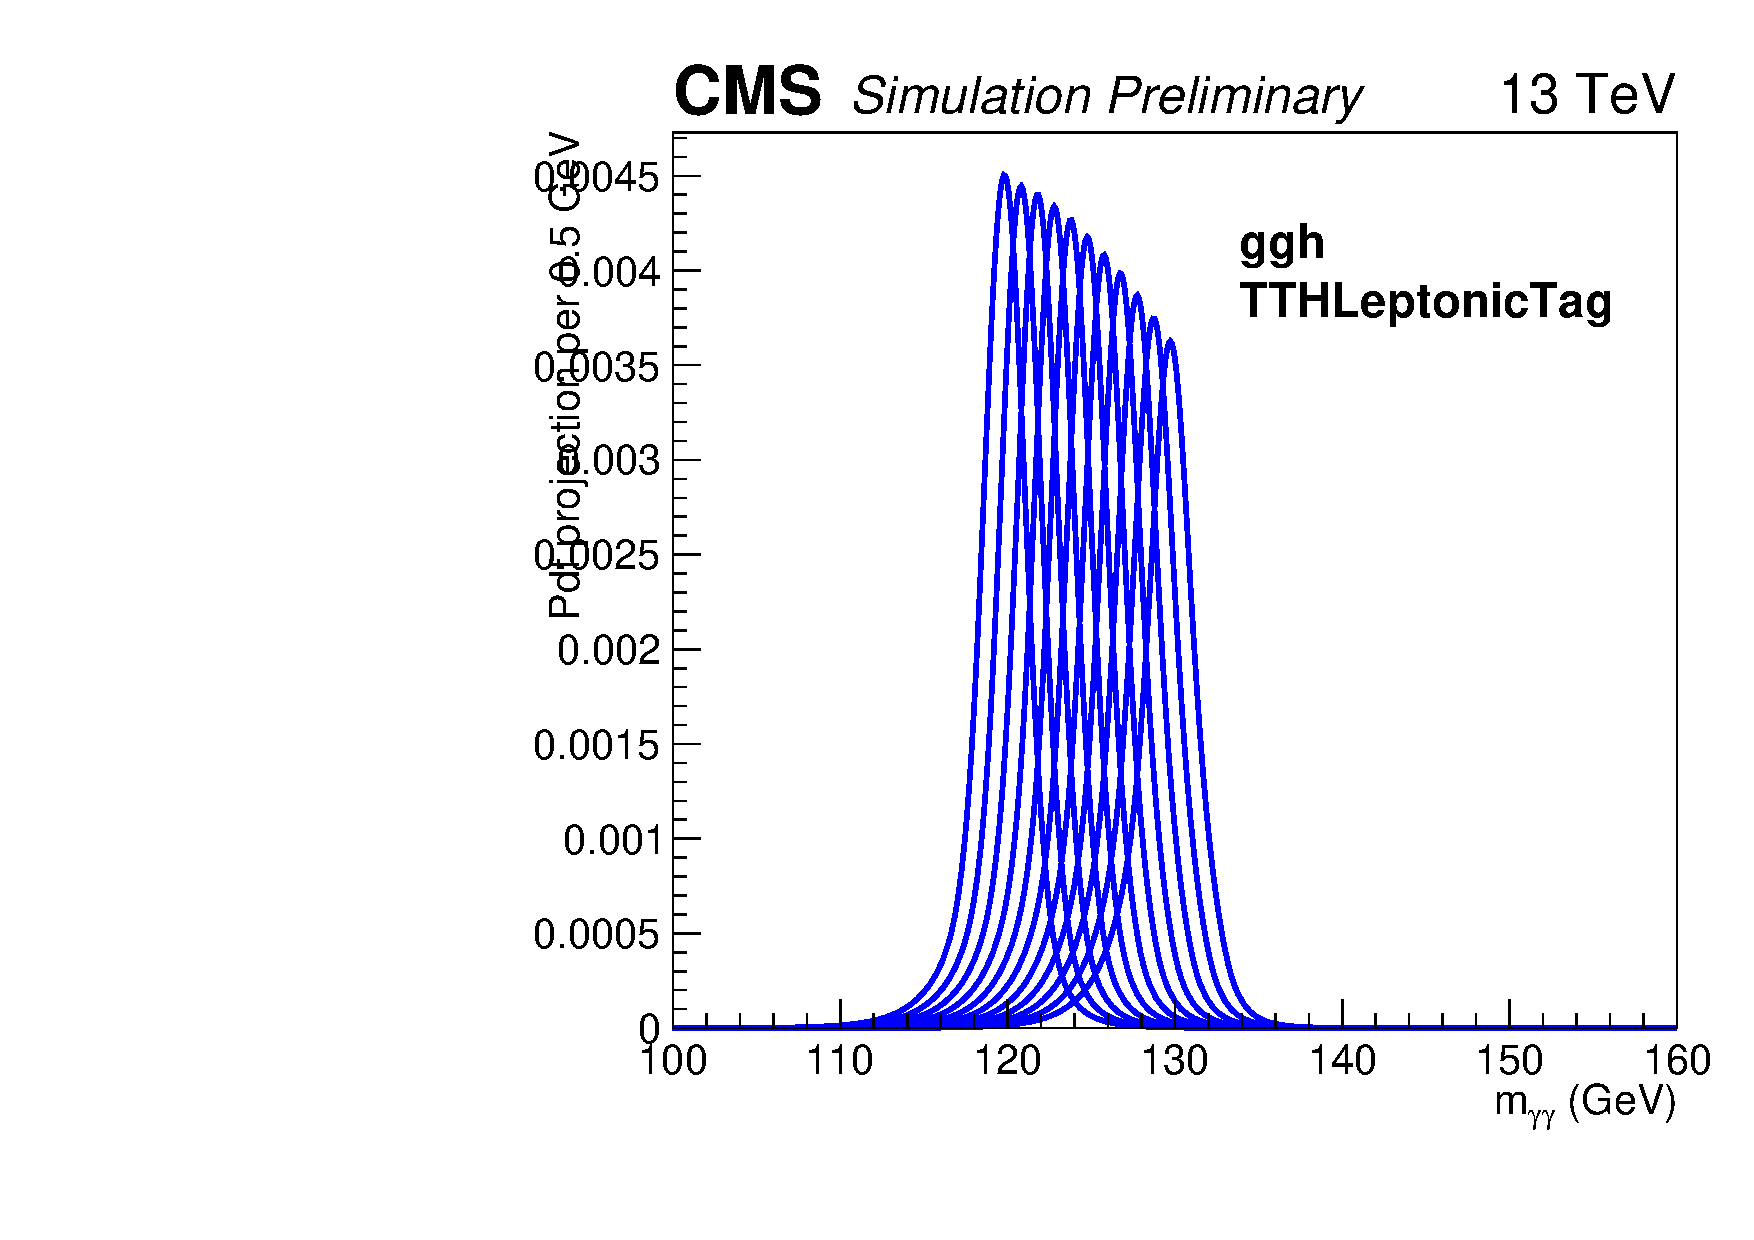
\includegraphics[width=0.3\textwidth]{modellingFigures/DCBpG/ggh_TTHLeptonicTag_fmc_interp.pdf} 
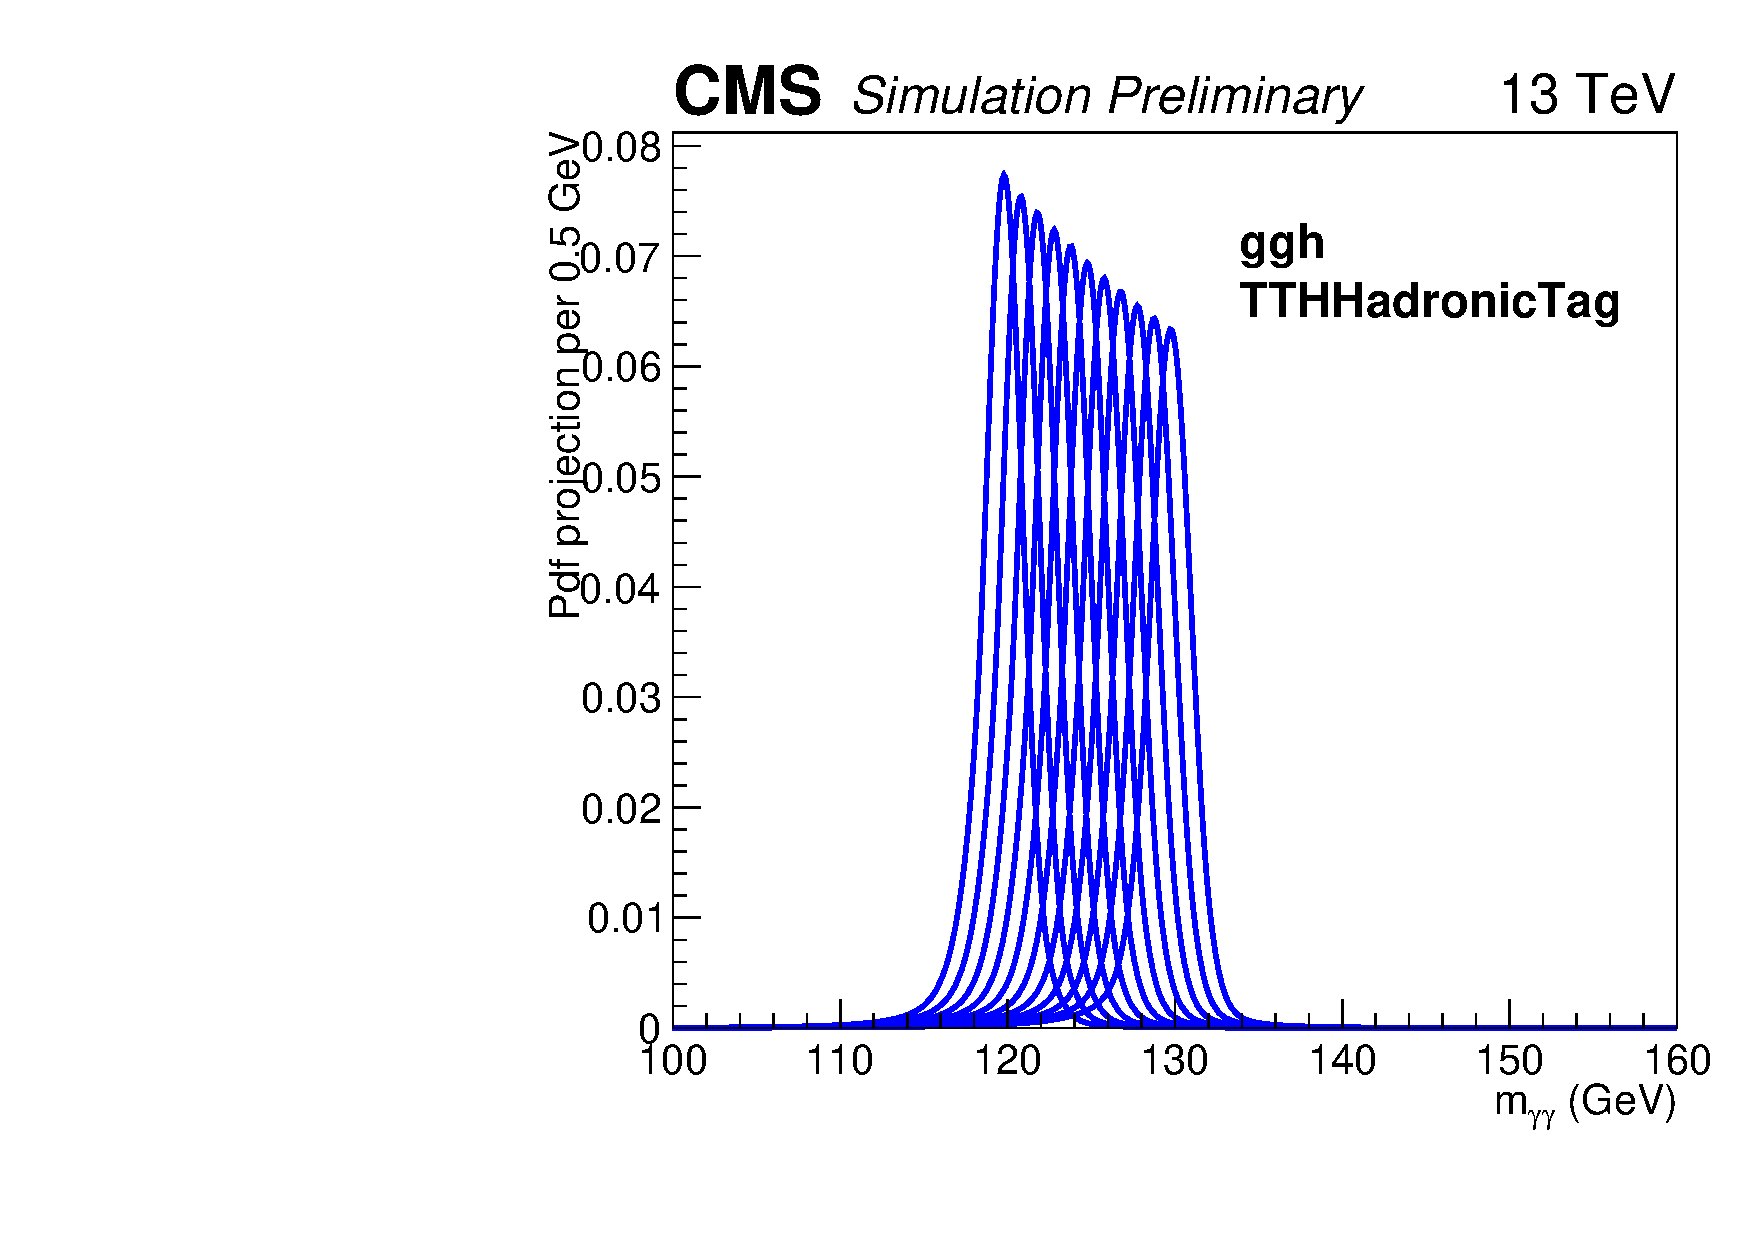
\includegraphics[width=0.3\textwidth]{modellingFigures/DCBpG/ggh_TTHHadronicTag_fmc_interp.pdf} 
\caption{The \mH-dependence of the signal models for the ggH process for each of the analysis categories is shown. Each curve shows the signal model for a given value of \mH. The contributions from the RV and WV components of each model were summed together according to their relative size, linearly interpolated between the samples for different \mH.}

\label{fig:model:sig_interpolation}
\end{figure}

\subsection{Normalisation of signal models}

The signal models for each process and category must be normalised to match the event yield expected for the \SM after detector acceptance ($A$) and selection efficiency ($\epsilon$) are taken into account. The total number of events from a given process is determined by multiplying the process \crosssection by the \Hgg \BR and the integrated luminosity of the data sample to be analysed.The values for the Higgs production modes and the \Hgg \BR, as well as their dependence on \mH, are taken from \LHCHXSWG. The simulated signal samples are then normalised such that number of events in the sample at generator level matches the number of events predicted by the \SM. After the simulated samples have been reconstructed and the events selected and categorised, the total number of events remaining is related to the expected number by the \effxacc. The \effxacc is evaluated separately for each process and category, and is parametrised in \mH using a polynomial fit to give a continuous model. The final normalisation is given by the \effxacc multiplied by the total number of expected events for the integrated luminosity of the data sample as a function of \mH.

The signal models for different processes can hen be summed together as required to obtain the expected \mgg distribution of signal events for a given analysis category or for all categories combined. \Fig~\ref{} shows the overall \effxacc for all categories combined as a function of \mH.

\begin{figure}[ht!]
\centering
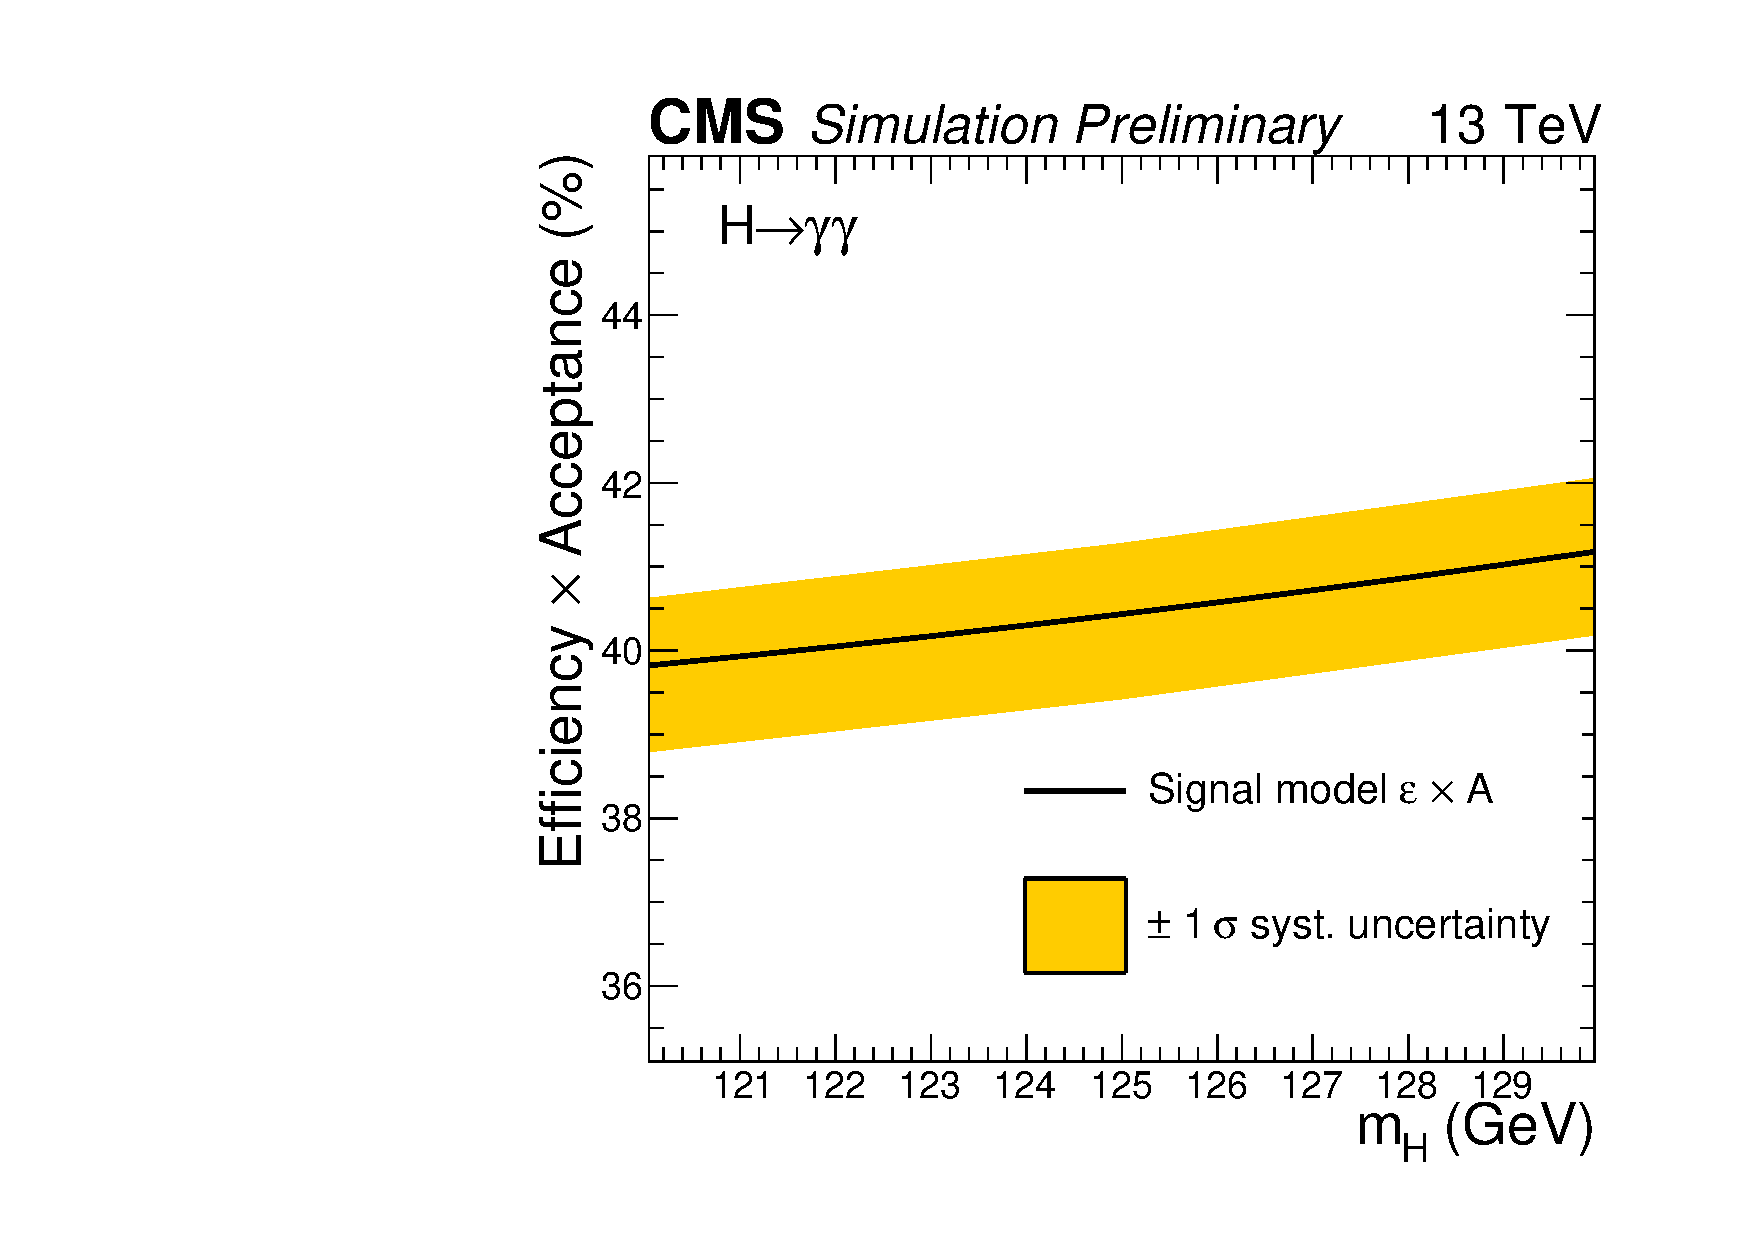
\includegraphics[width=0.6\textwidth]{modellingFigures/effAcc_vs_mass.pdf} 
\caption{The \effxacc of all categories combined shown as a function of \mH. The ornage band shows the effect of the systematic uncertainties associated with trigger efficiency, photon identification and selection, photon energy scale and resolution and vertex identification.}

\label{fig:model:sig_effxacc}
\end{figure}

The signal model evaluated at $\mH=125\GeV$ for all categories combined, obtained by summing the normalisaed contributions from each process, are shown in \Fig~\ref{fig:model:sig_model_all}, and for each analysis category in \Fig\s~\ref{fig:model:sig_model_per_category_inc} and~\ref{fig:model:sig_model_per_category_exc}.. 
\begin{figure}[ht!]
\centering
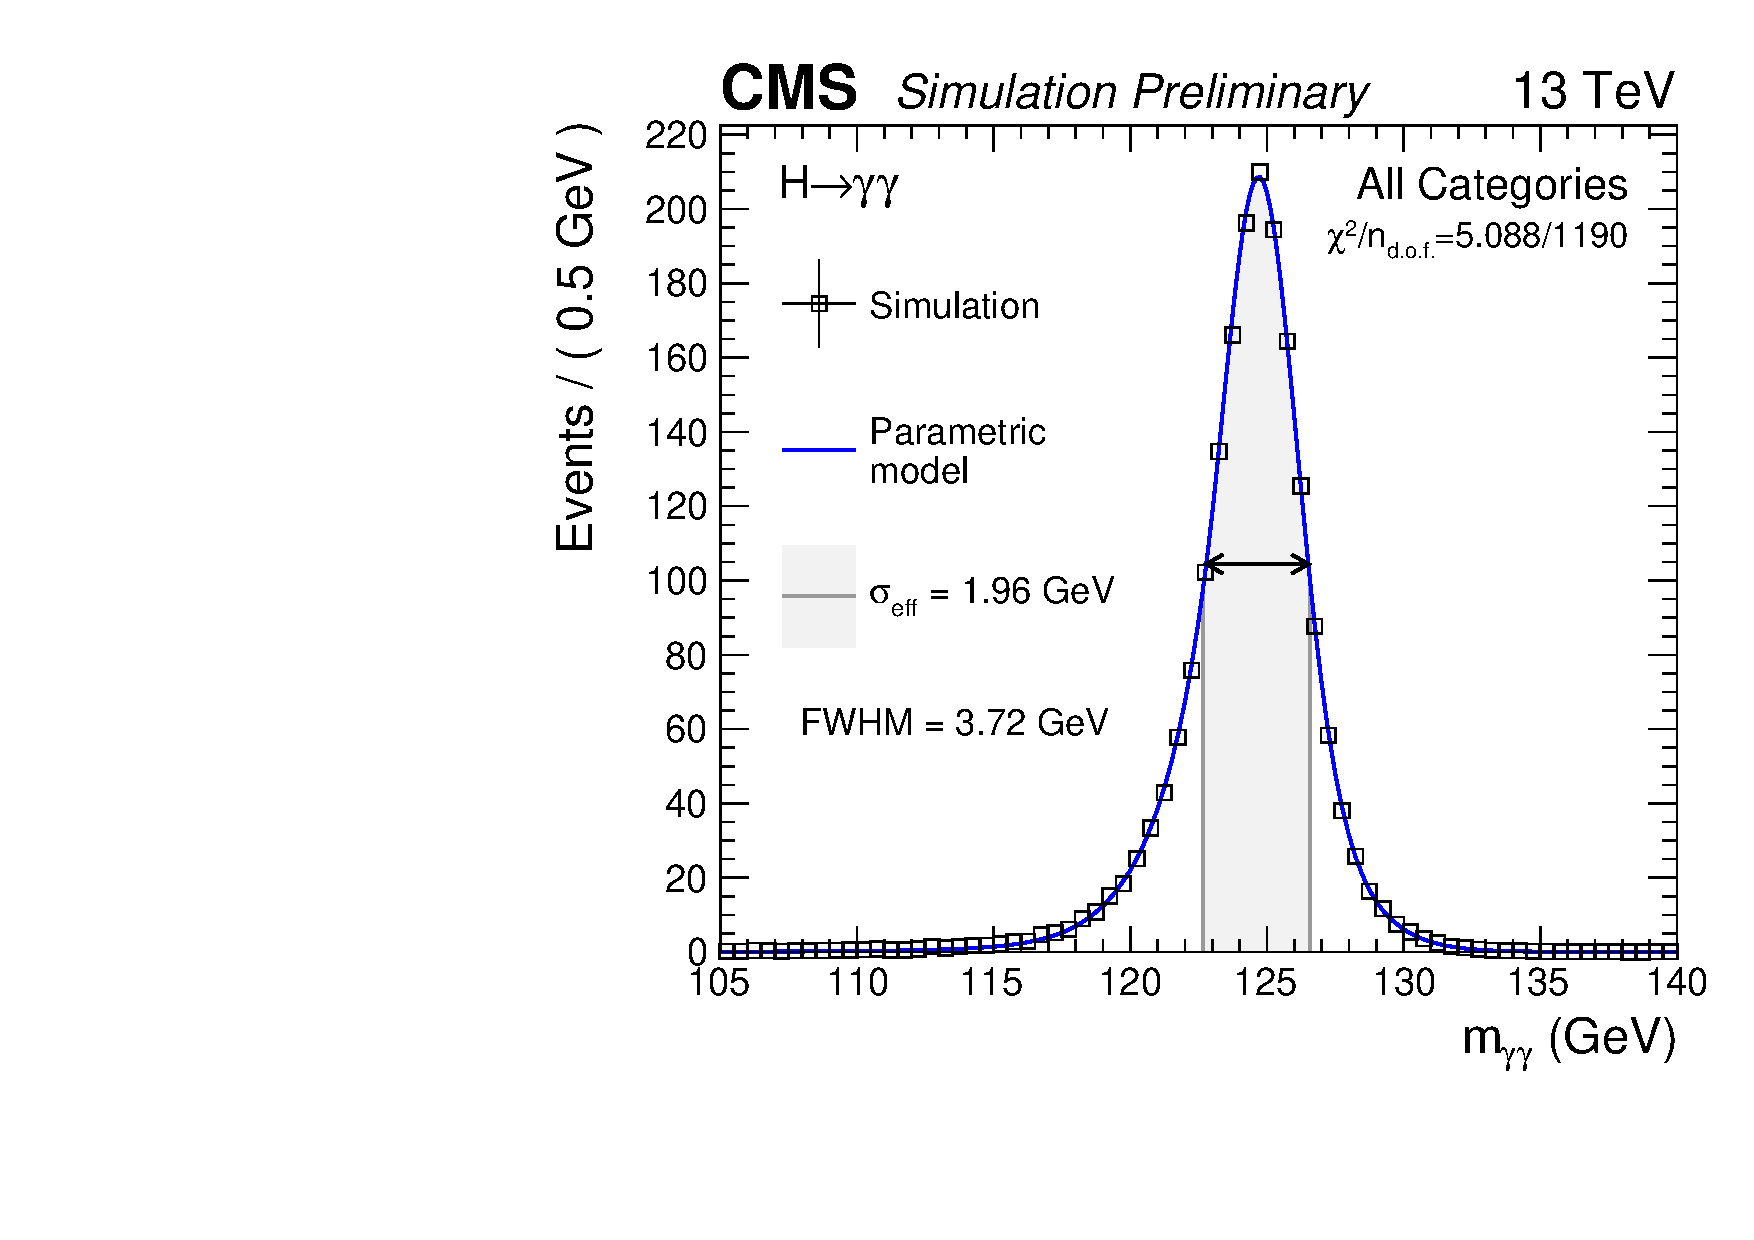
\includegraphics[width=0.6\textwidth]{modellingFigures/DCBpG/all.pdf} 

\caption{The signal model for all analysis categories combined for $\mH=125\GeV$, obtained by summing the contributions from each production process according to the \effxacc. The \effSigma value (half the width of the narrowest interval containing 68.3\% of the invariant mass distribution) and the FWHM (the width of the distribution at half of the maximum value) are also shown. }

\label{fig:model:sig_model_all}
\end{figure}

\begin{figure}[ht!]
\centering
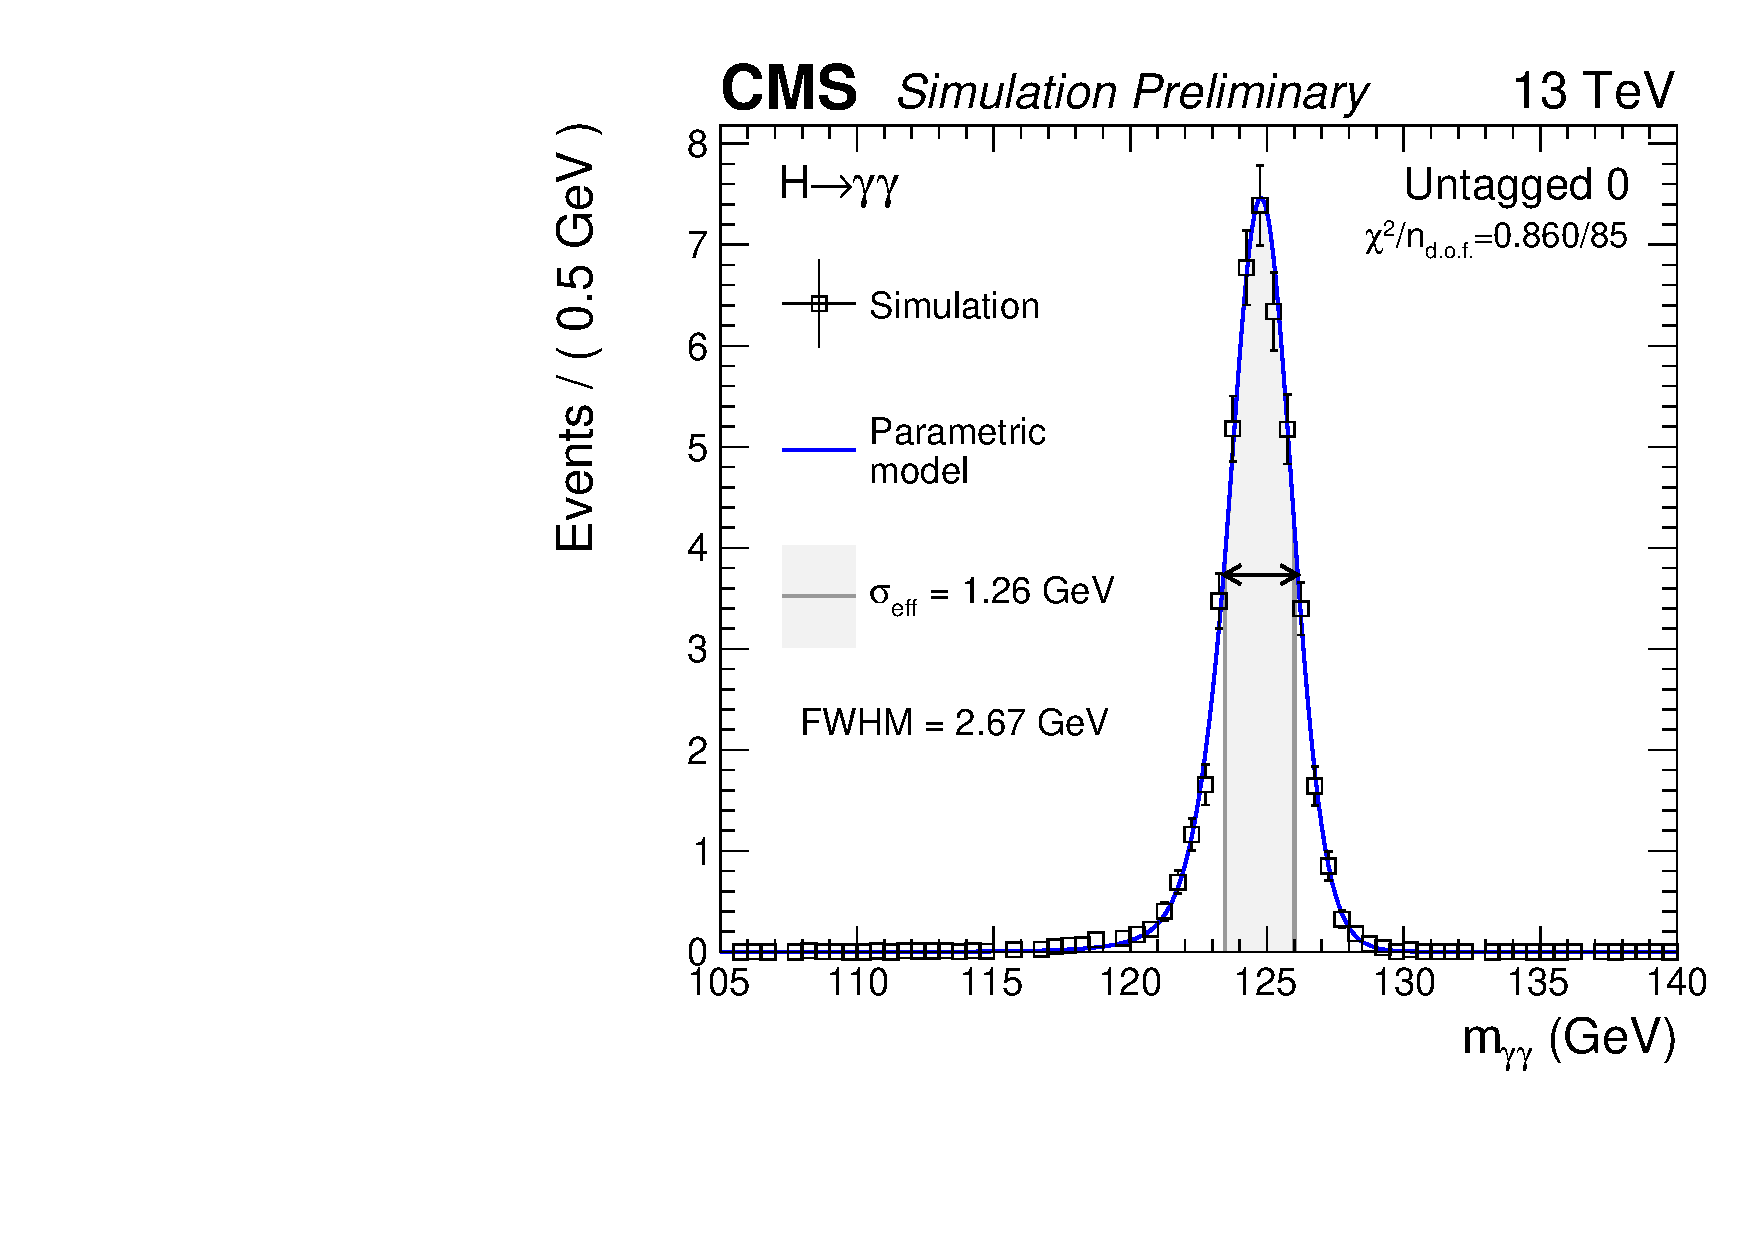
\includegraphics[width=0.45\textwidth]{modellingFigures/DCBpG/UntaggedTag_0.pdf} 
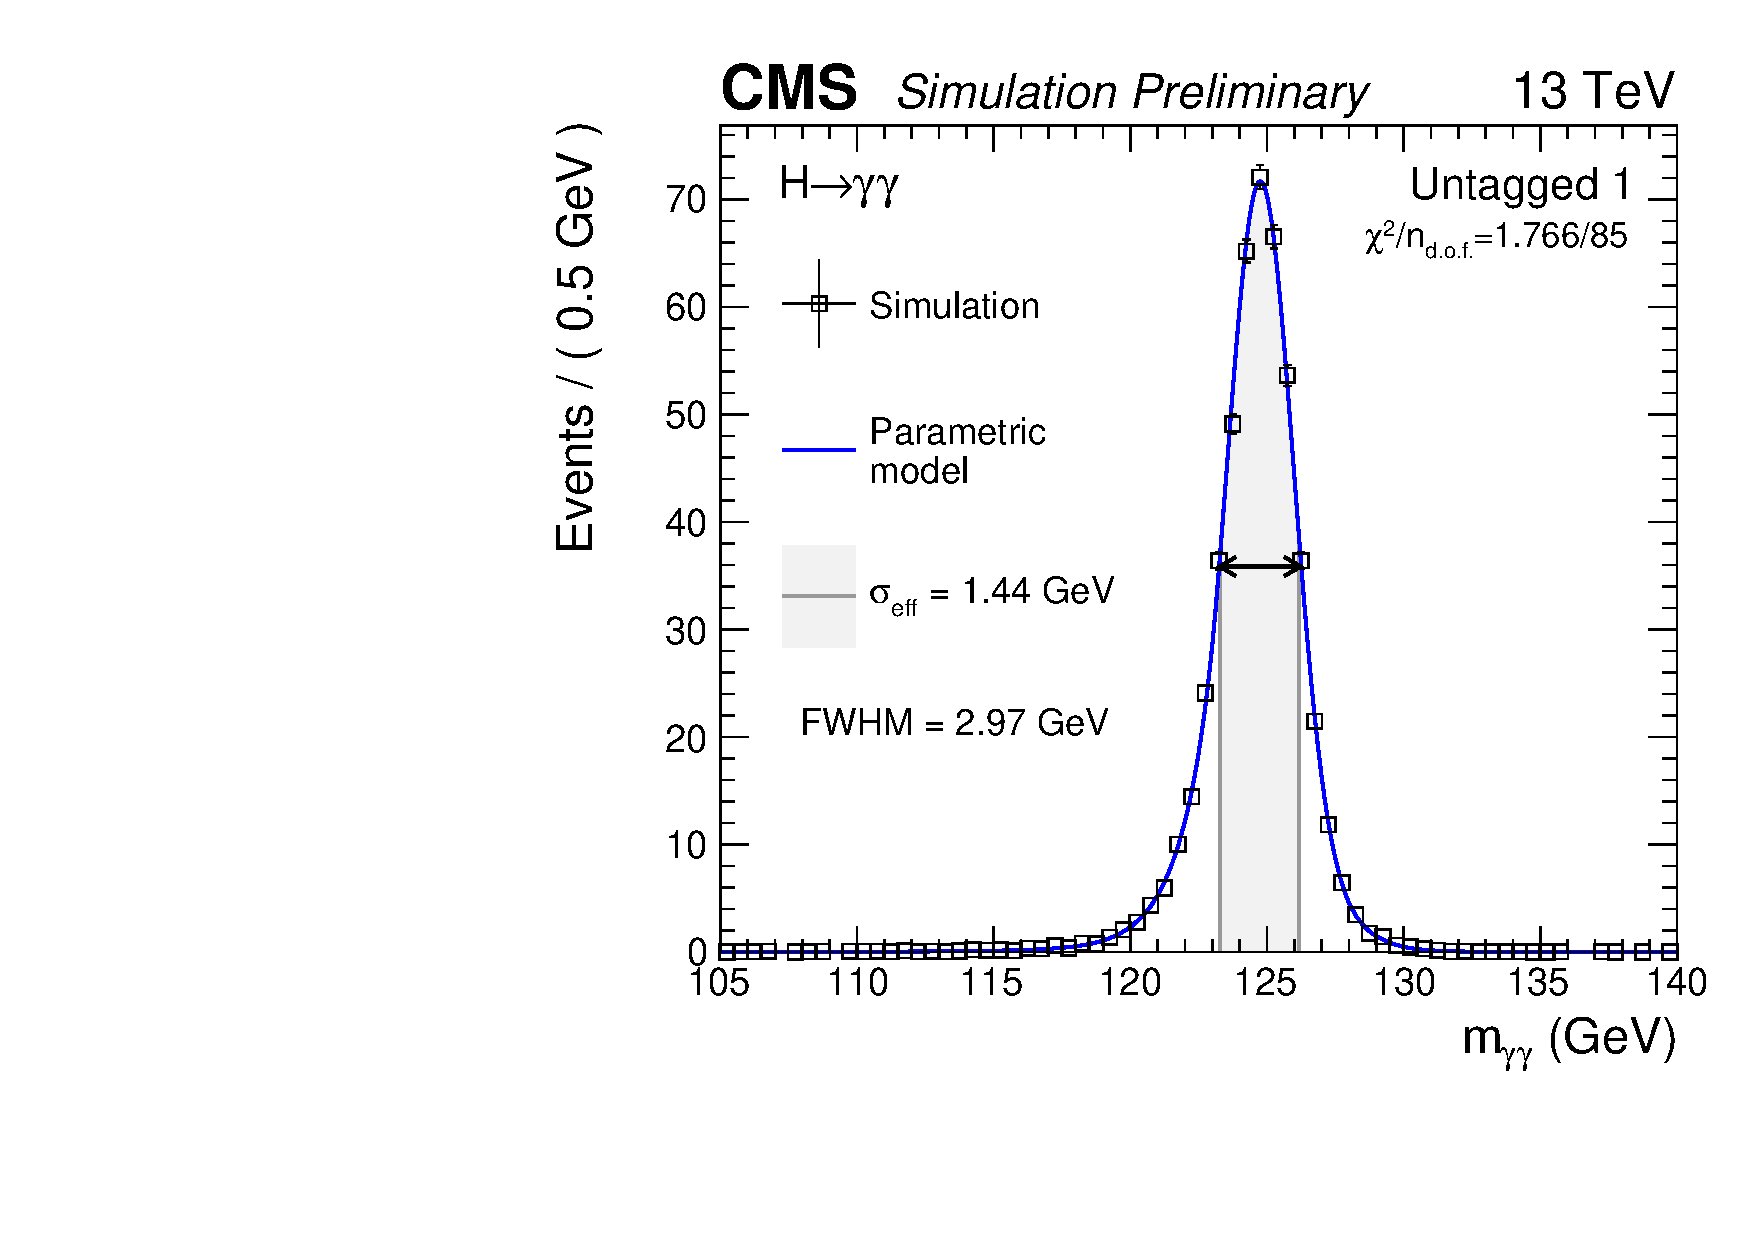
\includegraphics[width=0.45\textwidth]{modellingFigures/DCBpG/UntaggedTag_1.pdf} \\
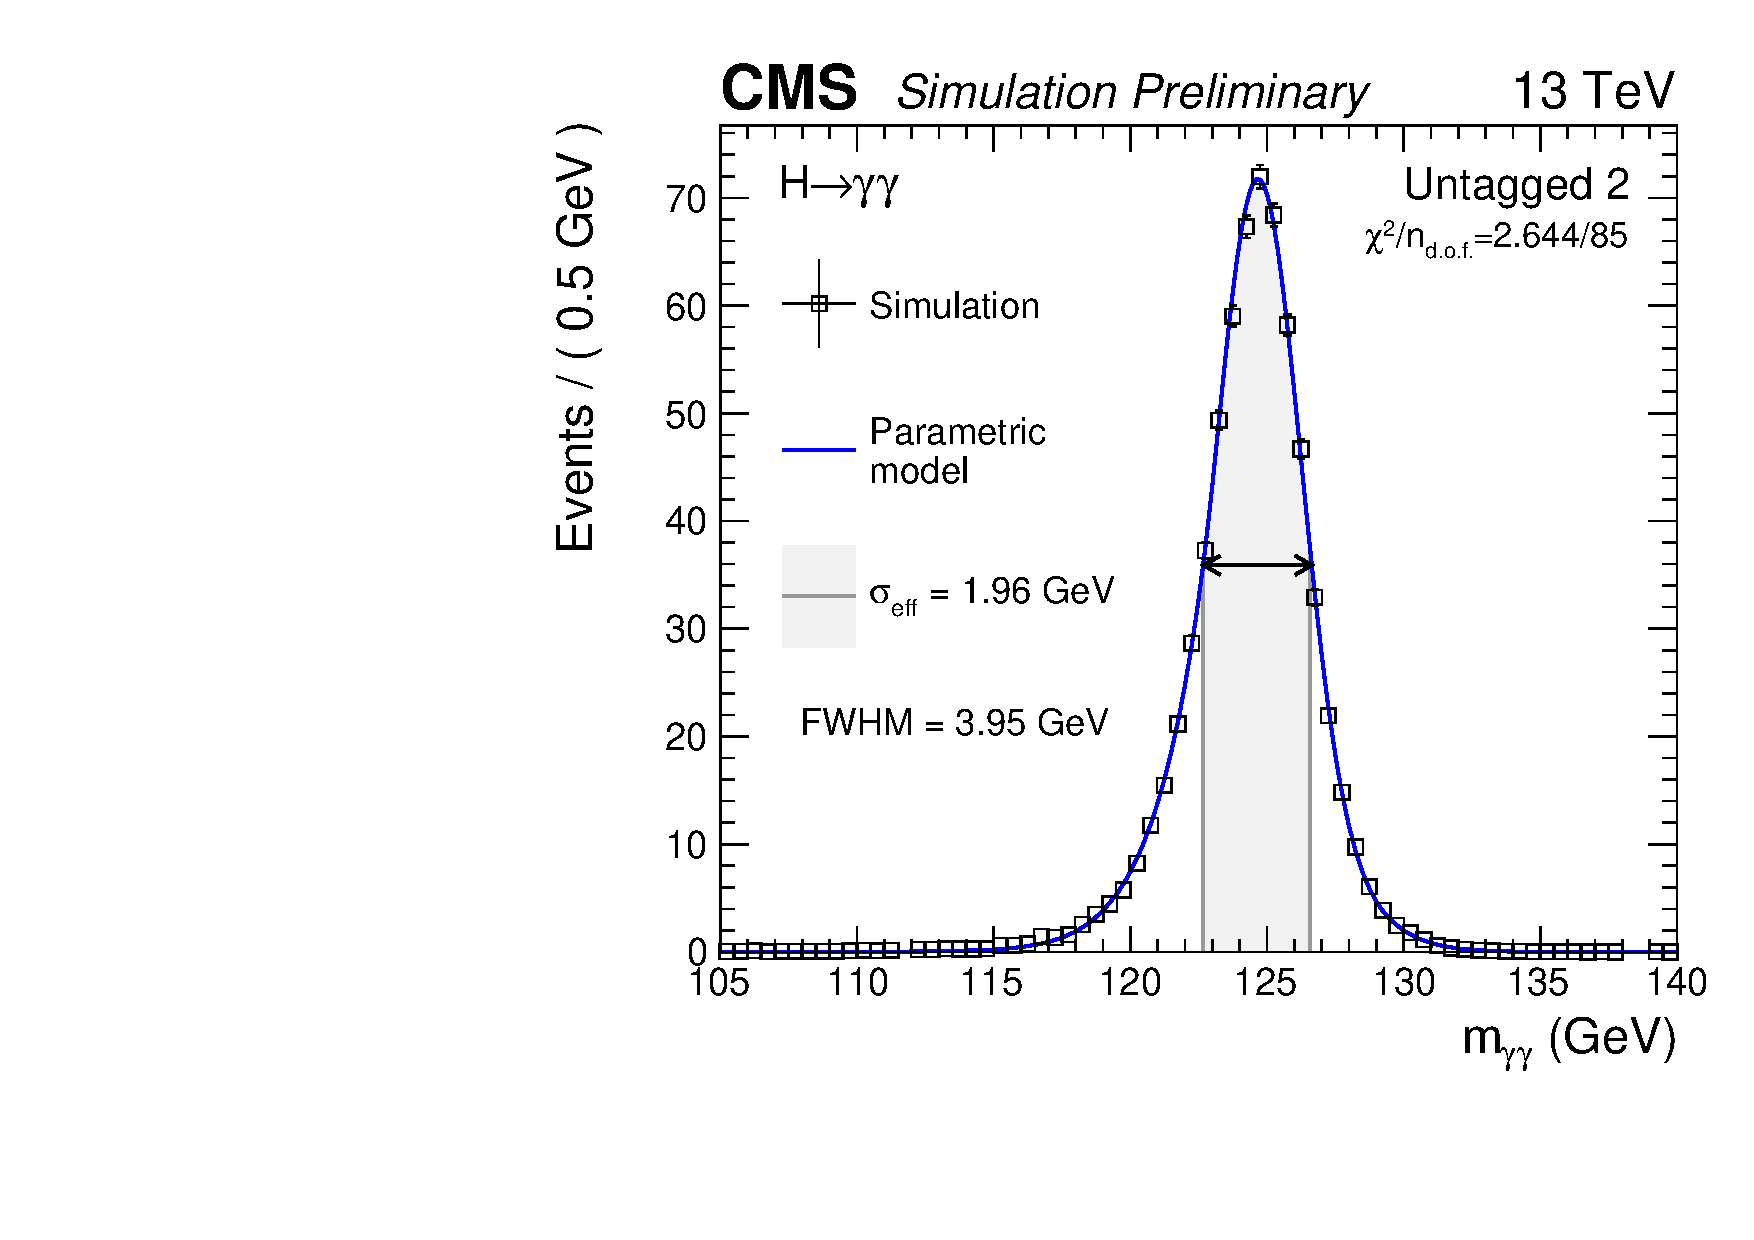
\includegraphics[width=0.45\textwidth]{modellingFigures/DCBpG/UntaggedTag_2.pdf} 
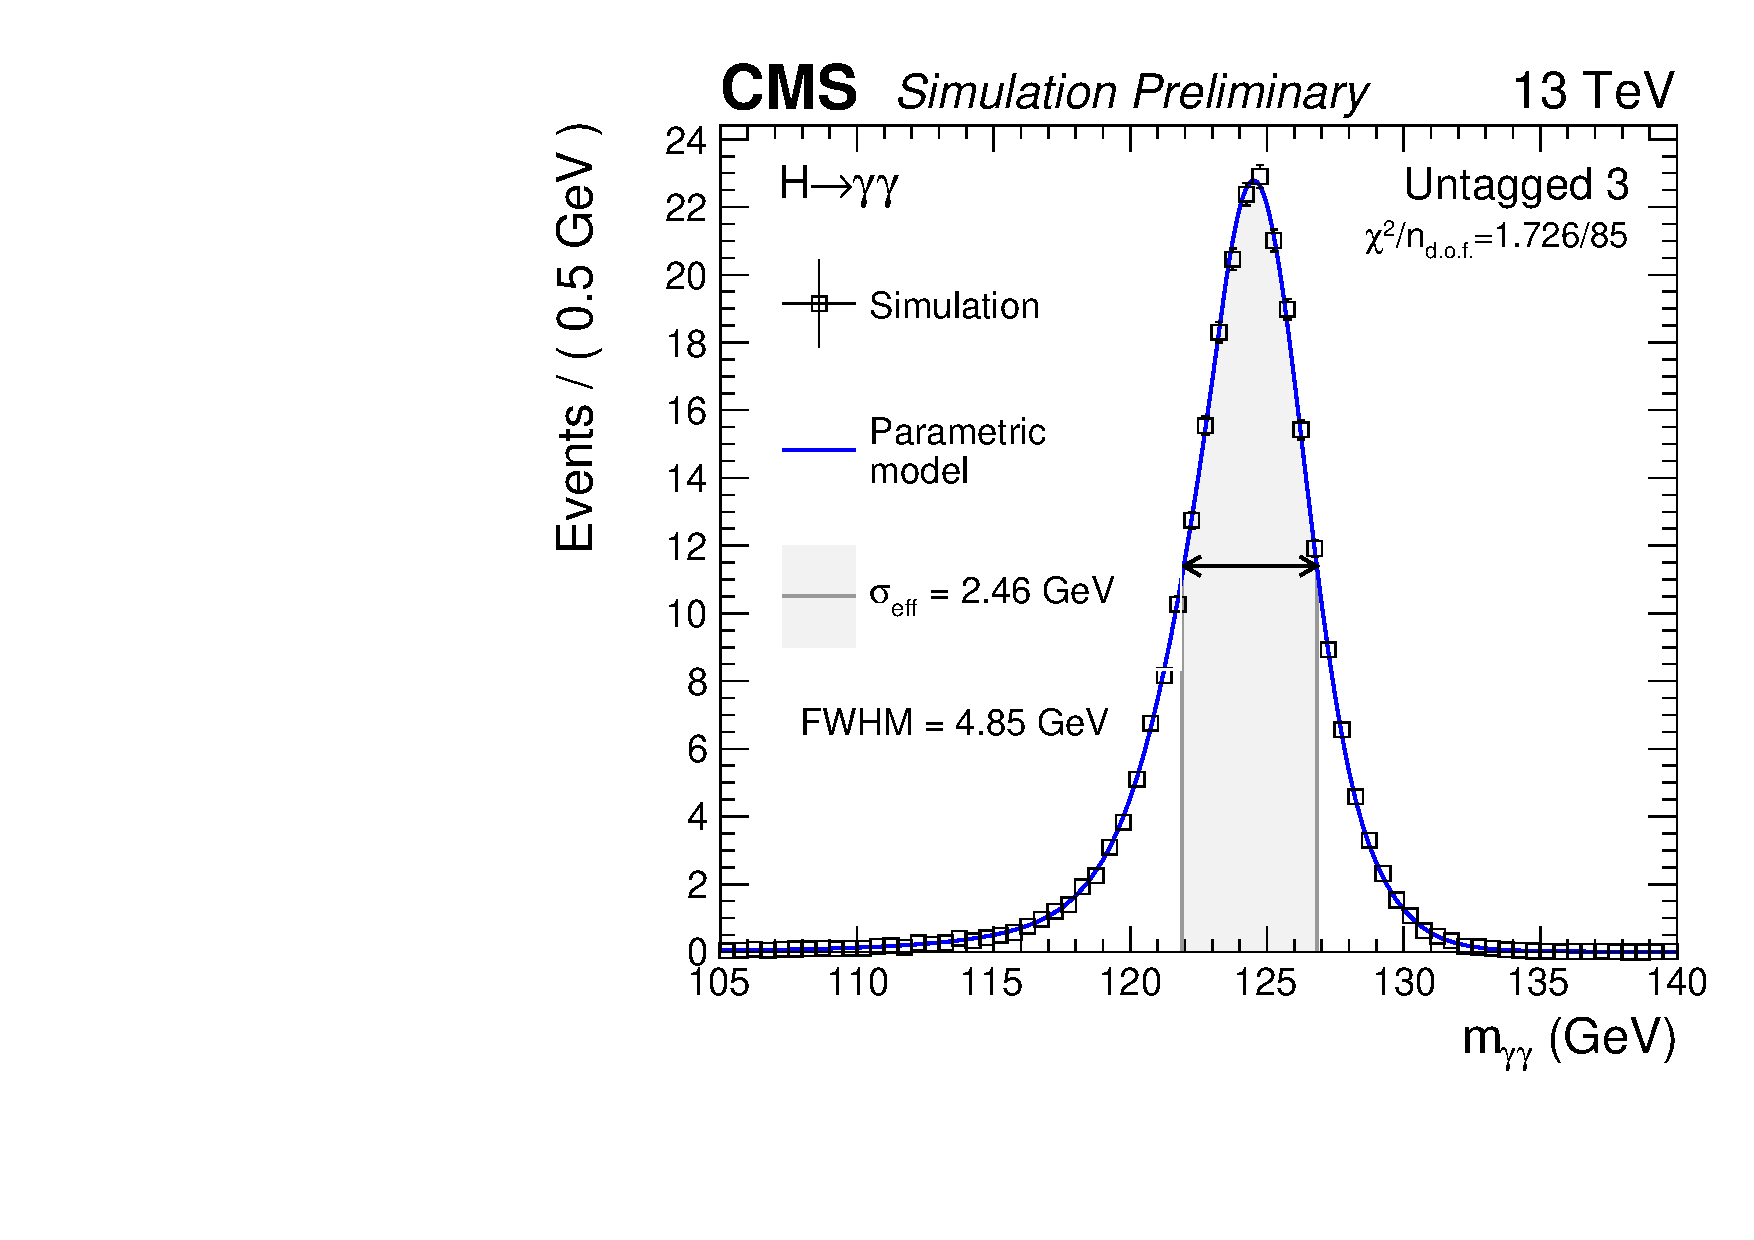
\includegraphics[width=0.45\textwidth]{modellingFigures/DCBpG/UntaggedTag_3.pdf}  

\caption{The signal models for the inclusive analysis categories for $\mH=125\GeV$, obtained by summing the contributions from each production process according to the \effxacc. The \effSigma value (half the width of the narrowest interval containing 68.3\% of the invariant mass distribution) and the FWHM (the width of the distribution at half of the maximum value) are also shown.}

\label{fig:model:sig_model_per_category_inc}
\end{figure}
\begin{figure}[ht!]
\centering
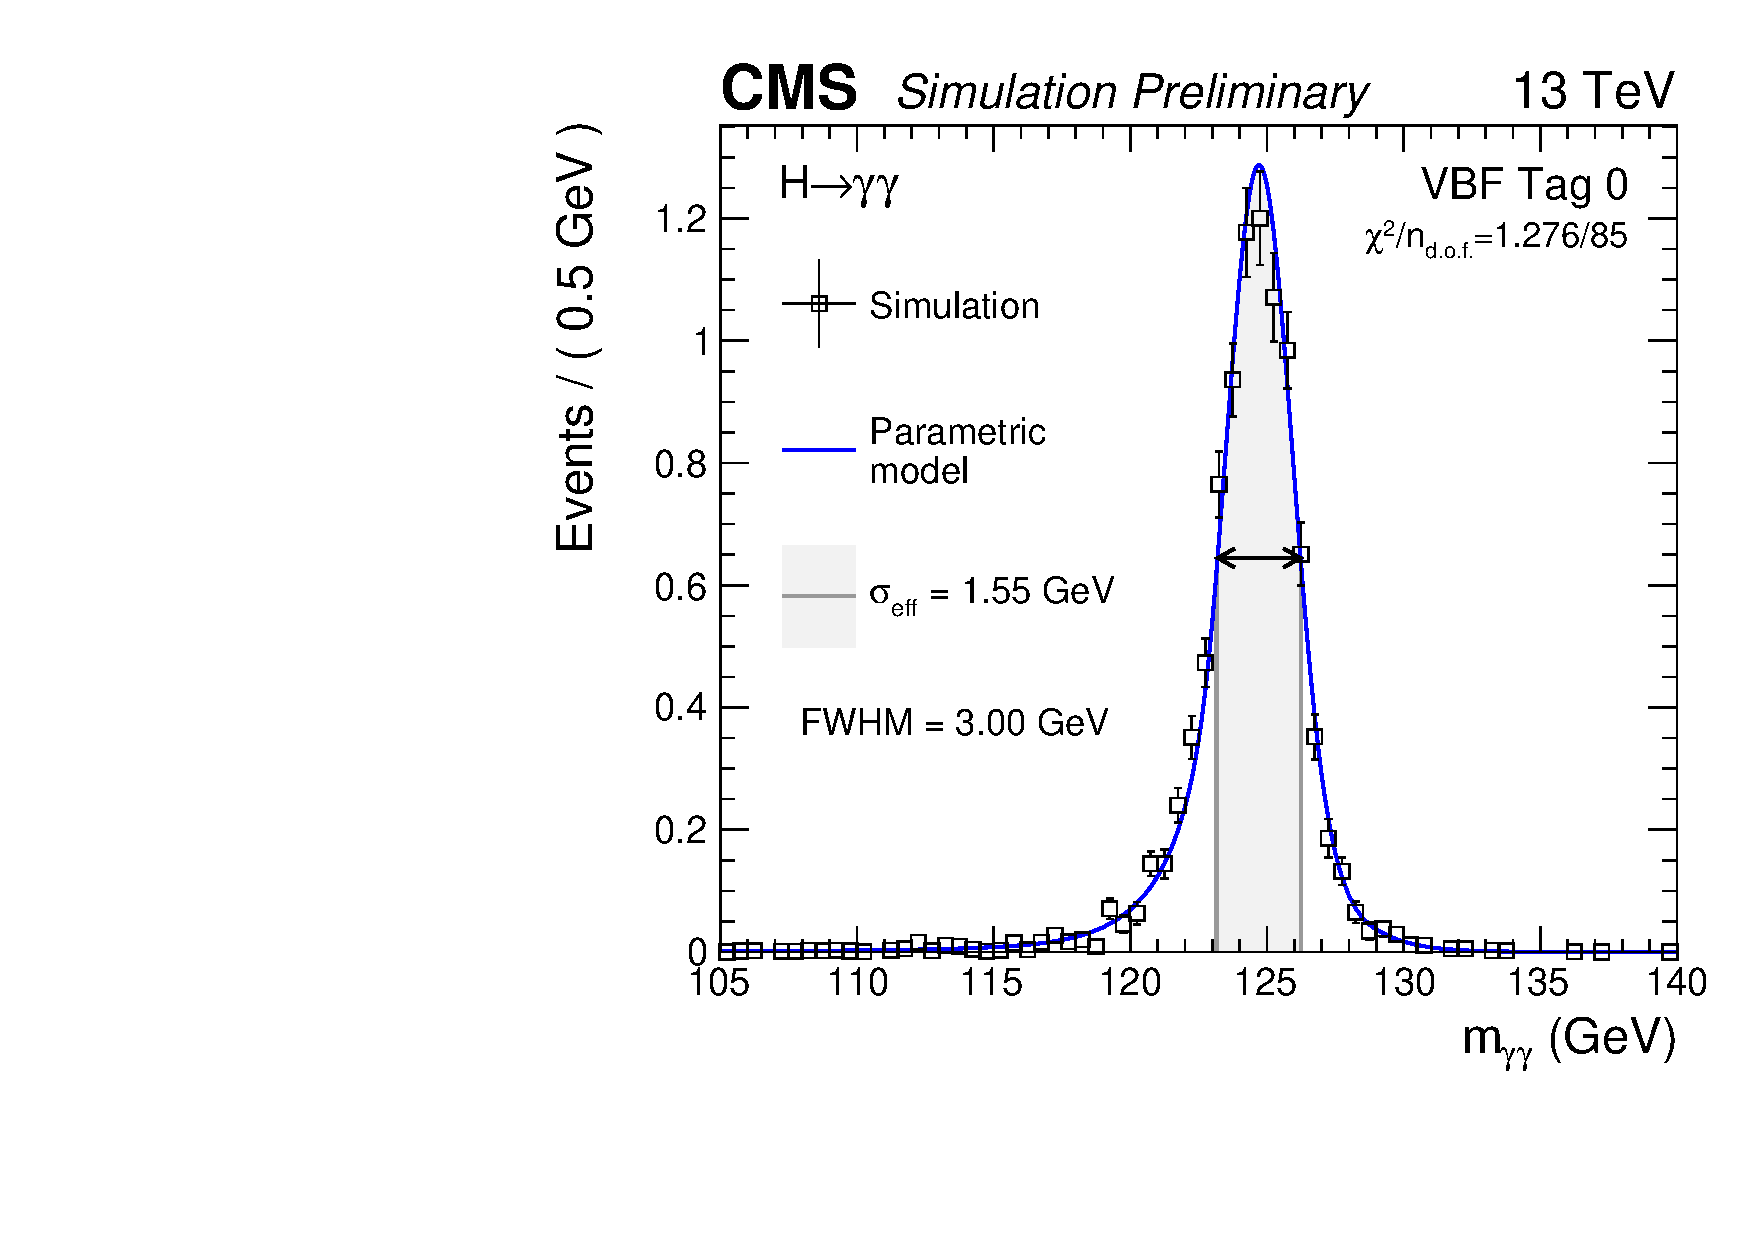
\includegraphics[width=0.45\textwidth]{modellingFigures/DCBpG/VBFTag_0.pdf} 
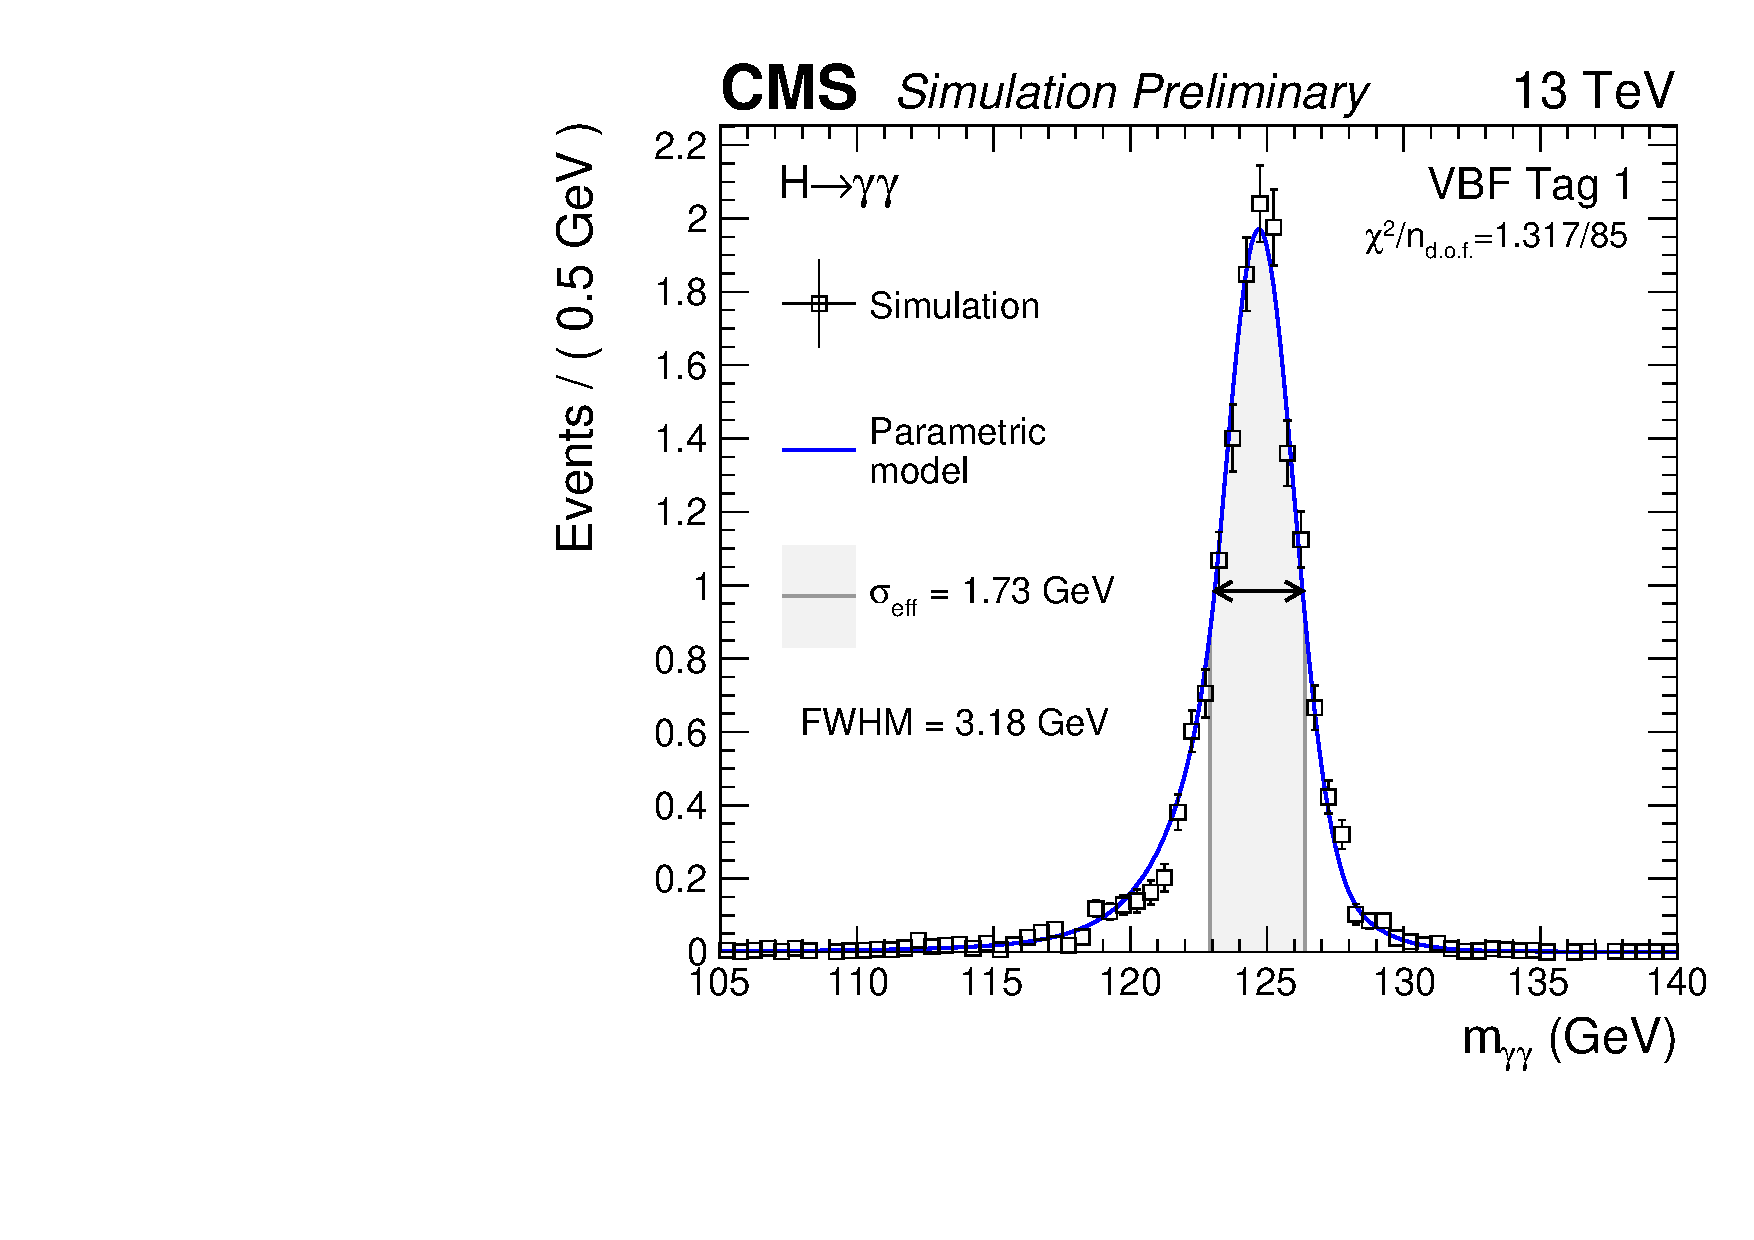
\includegraphics[width=0.45\textwidth]{modellingFigures/DCBpG/VBFTag_1.pdf} \\
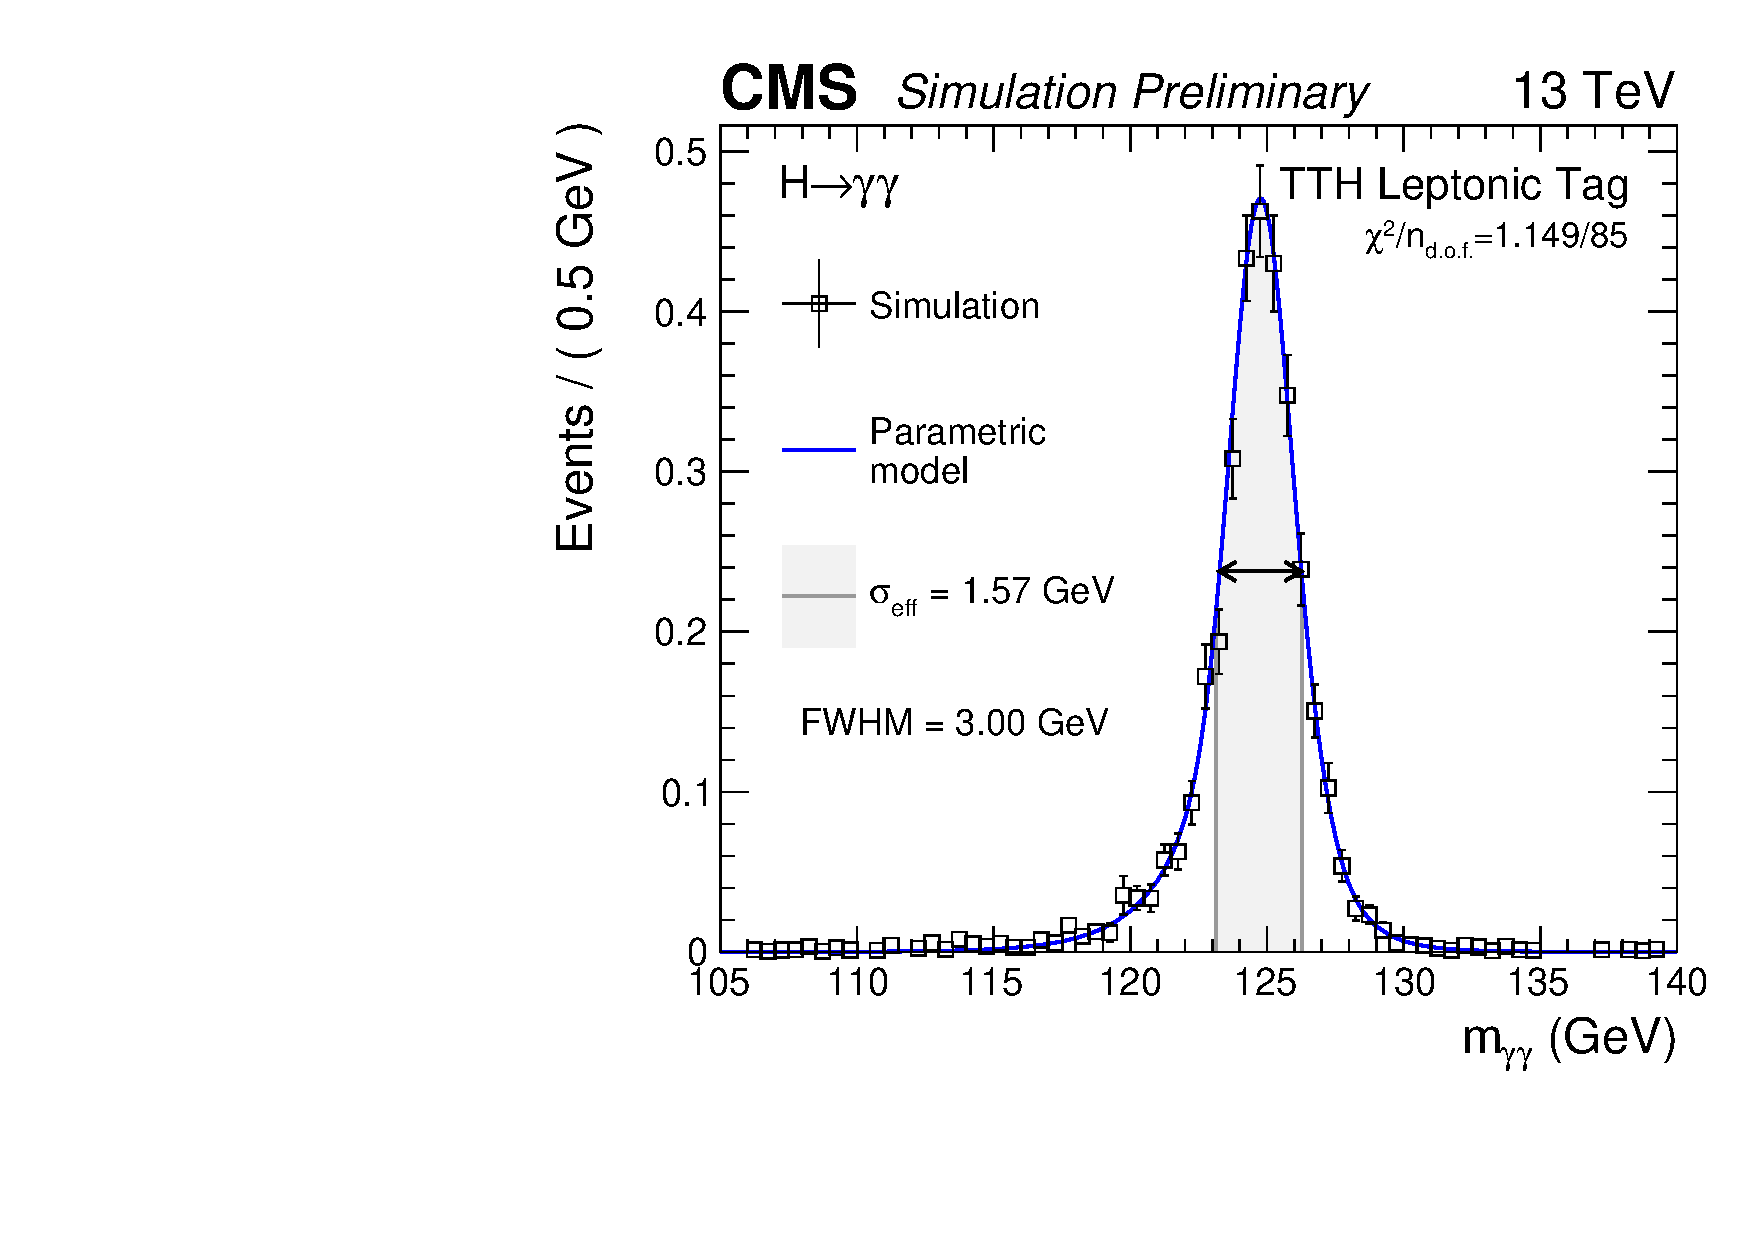
\includegraphics[width=0.45\textwidth]{modellingFigures/DCBpG/TTHLeptonicTag.pdf} 
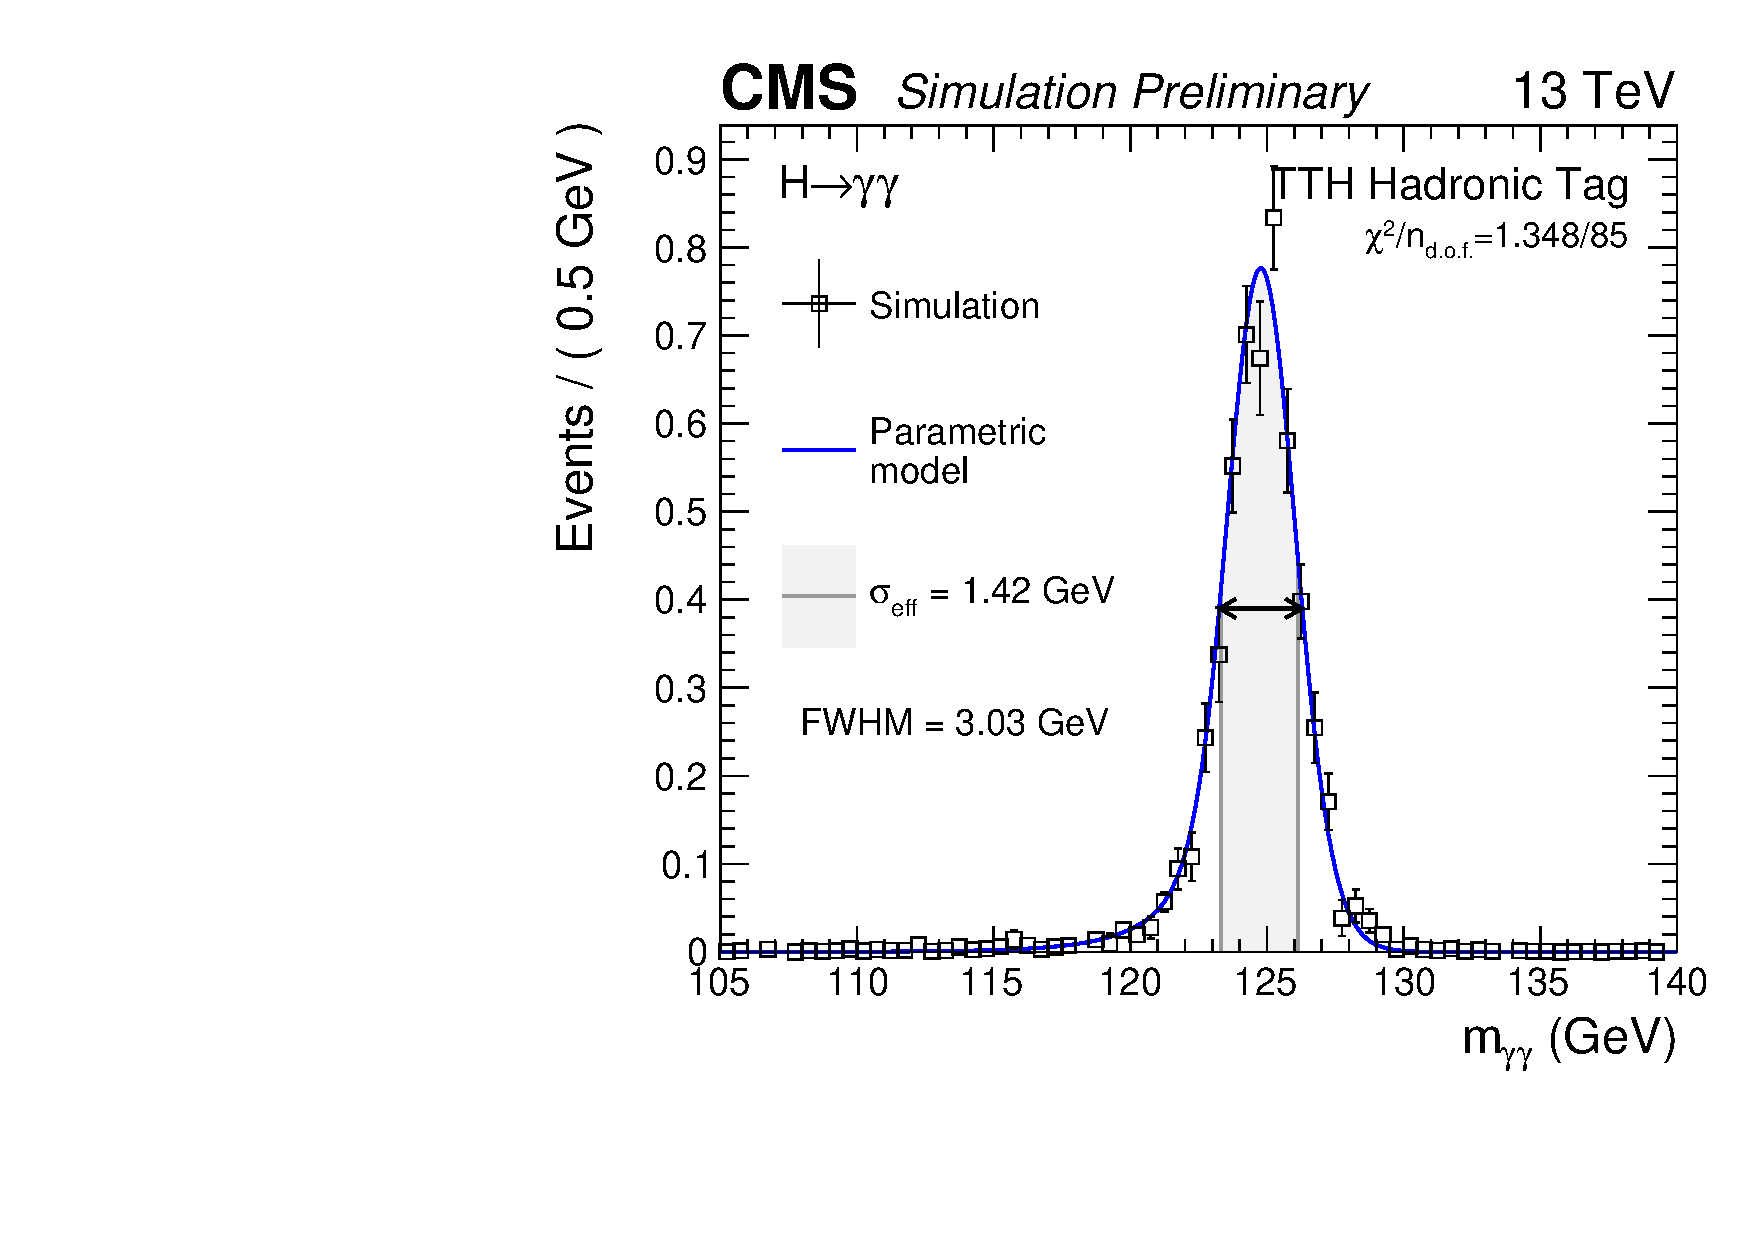
\includegraphics[width=0.45\textwidth]{modellingFigures/DCBpG/TTHHadronicTag.pdf} 

\caption{The signal models for the \VBFTag and \TTHTag analysis categories for $\mH=125\GeV$, obtained by summing the contributions from each production process according to the \effxacc. The \effSigma value (half the width of the narrowest interval containing 68.3\% of the invariant mass distribution) and the FWHM (the width of the distribution at half of the maximum value) are also shown.}

\label{fig:model:sig_model_per_category_exc}
\end{figure}



%\subsection{Handling of photon energy systematics}

%The systematics associa

\section{Background modelling}
\label{model:sec:background_model}
\subsection{The discrete profiling method}

In this analysis, the background model is produced from data using the discrete profiling method~\cite{DiscreteProfiling}, which treats the choice of functional form to describe the background as a discrete nuisance parameter in the likelihood fit to the data. 

The discrete profiling method was introduced because the underlying functional form of a background distribution is generally not known. Several different families of function could in principle be chosen to parametrise the background distributions, all giving acceptable agreement with the data. Within a given family, it is not always clear which order to choose, or how to process the uncertainty associated with a particular choice of functional form.  %An common solution is to make an arbitrary choice of functional form and try to estimate the bias introduced by pikcing that shape, and trying to assign some systematic uncertainty to compensate.
The discrete profiling method seeks to provide an alternative solution to making an arbitrary choice of function. %Since the chosen functional form itself is not of interest, it can be treated as a discrete nuisance parameter and profiled in the likelihood fit.
and provides a natural way to handle of the uncertainty associated with the choice of background parametrisation. 

When extracting the best-fit value of a parameter of interest using a \NLL minimisation, nuisance parameters representing systematic uncertainties are typically profiled: their value is allowed to be varied during the minimisation, and the final value is not of interest. The additional freedom yields a wider \NLL curve, representing the additional uncertainty attributed the nuisance. 
If the value of the nuisance parameter is instead fixed at the best-fit value, the width of the resulting \NLL curve will be narrower narrower but still with minimum at the same place as for the full profiled \NLL curve. This width represents the uncertainty of the measurement without the effect of the fixed nuisance parameter. If the procedure is repeated for a different fixed values of the nuisance parameter, different \NLL curves, not necessarily at the minimum, will be produced. In the limit that many different values of the fixed nuisance parameter are sampled, the minimum envelope of all the fixed-nuisance \NLL curves will converge to the full profiled \NLL. The uncertainty can then be obtained from the envelope as for a usual \NLL curve. This property is true also for discrete nuisance parameters. The procedure is illustrated in \Fig~\ref{fig:model:bkg_envelope}. When parametrising the background distribution, since the functional form itself is not of interest it can be treated as a discrete nuisance parameter and the method as described above can be used to assess the uncertainty associated with the parametrisation of the background. The fact that different functional forms can have different numbers of degrees of freedom is taken into account by adding a penalty term to the \NLL proportional tot he number of parameters in the functional form. 

\begin{figure}[ht!]
\centering
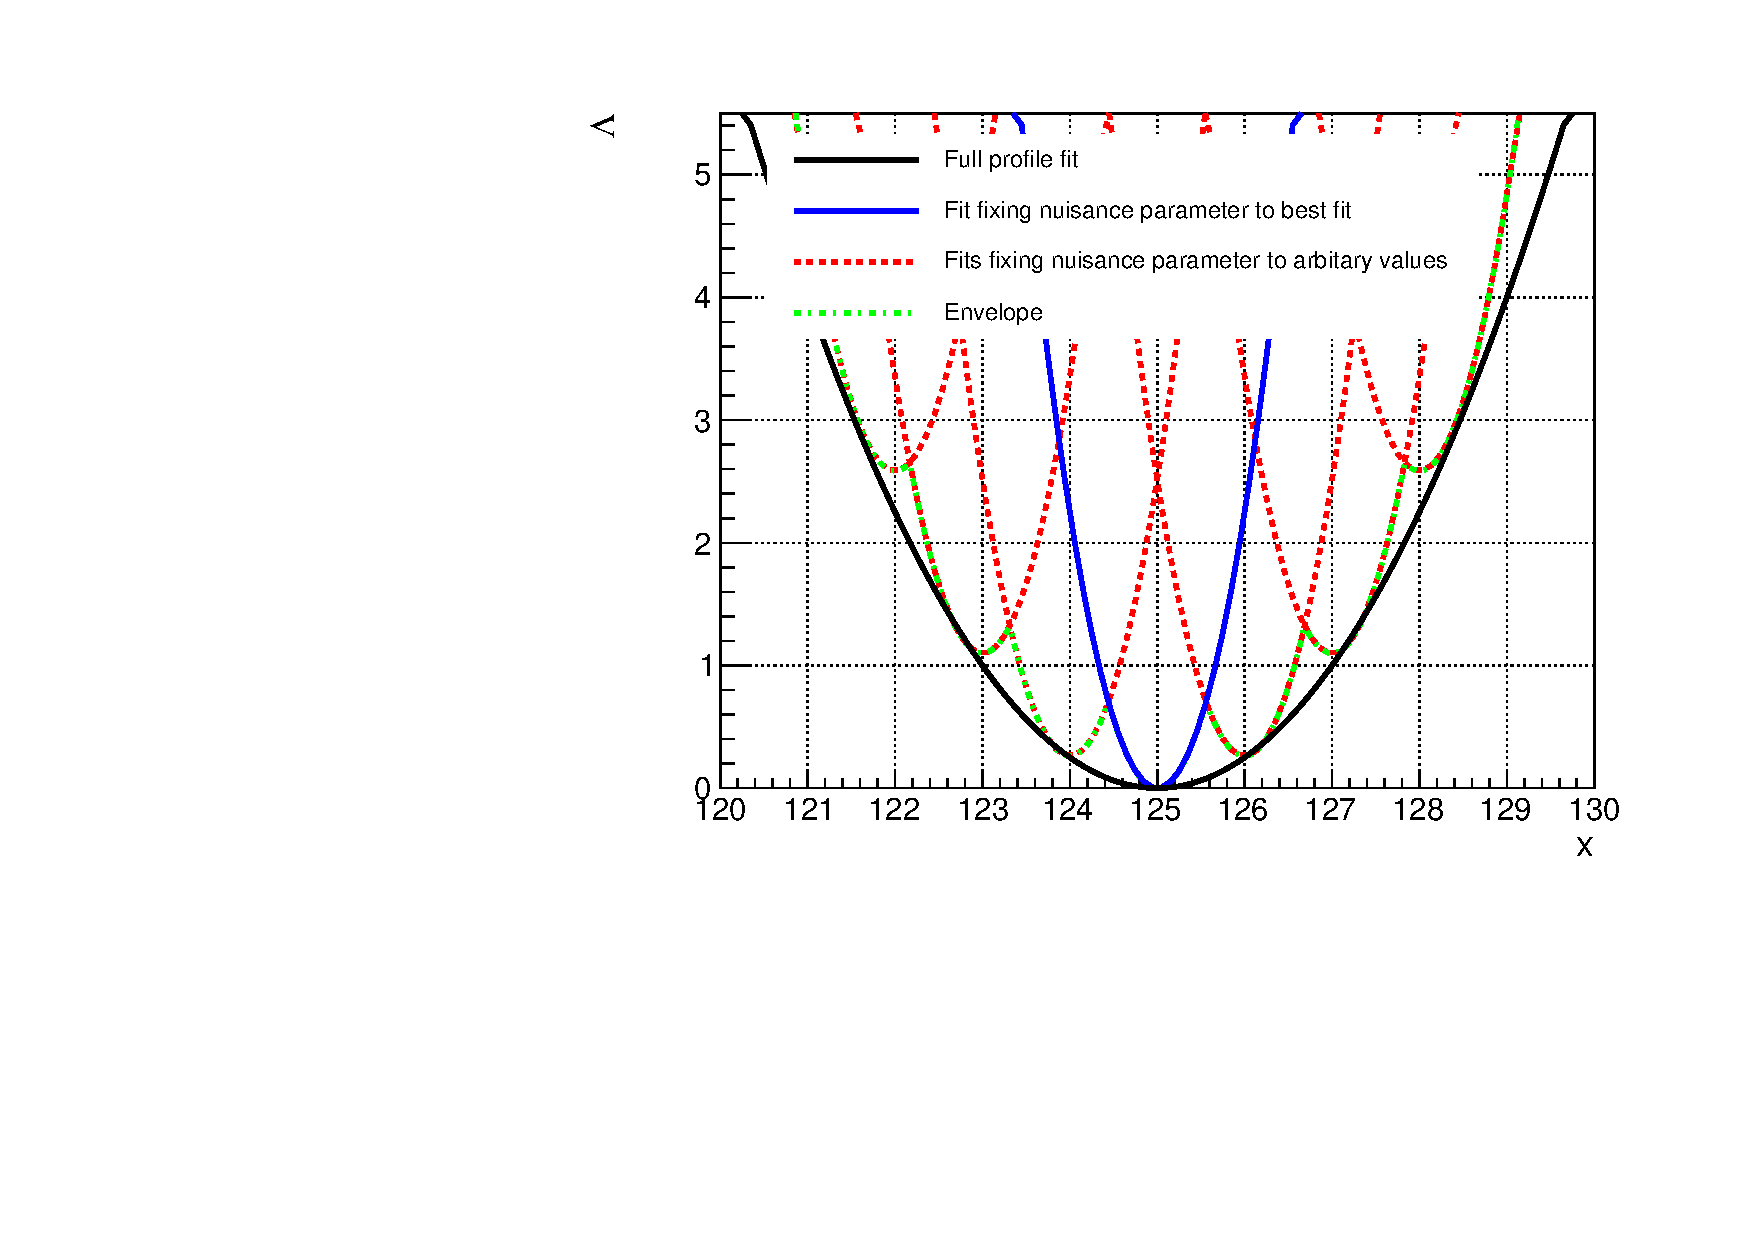
\includegraphics[width=0.8\textwidth]{modellingFigures/envelope_cartoon.pdf} 
\caption{An illustration of construction of the envelope to estimate the effect of a nuisance parameter. The NLL (denoted as $\Lambda$) curve obtained when performing a likelihood scan of parameter of interest $x$ if the nuisance parameter is profiled is shown in black. The NLL curve obtained by fixing the nuisance to the best-fit value is shown in blue. The NLL curves for various fixed values of the nuisance other than the best-fit are shown in red. The minimum envelope of these curves, shown in green, approximates the original NLL curve obtained by profiling the nuisance parameter.~\cite{DiscreteProfiling}.}

\label{fig:model:bkg_envelope}
\end{figure}

A complete set of all analytic functions should be considered for an exact result. In practice, it is only necessary to include a subset of all analytic function which give a good description of the data. In this analysis, the following four families of functions are considered:

\begin{itemize}
\item Sums of exponentials: $$ f_{N}(x)= \sum^{N}_{i=1} p_{2i} e^{p_{2i+1} x} ,$$
\item Sums of polynomials (in the Bernstein basis): $$ f_{N}(x) = \sum^{N}_{i=0} p_{i} b_{(i,N)}, \text{ where } b_{(i,N)}:= \begin{pmatrix} N \\ i \end{pmatrix} x^i (1-x)^{N-i} ,$$
\item Laurent series: $$ f_{N}(x)= \sum^{N}_{i=1} p_{i} x^{-4 + \sum^{i}_{j=1} (-1)^{j} (j-1)},$$
\item Sums of power-law functions: $$ f_{N}(x)= \sum^{N}_{i=1} p_{2i} x^{-p_{2i+1}},$$
\end{itemize}
where for all $k$, the $p_k$ are a set of floating parameters in the fits, and $N$ represents the \emph{order} of a particular function in the family.  

%The representations of the function families are chosen such that their members are nested: a function of a particular order can reproduce the shape of the functions of lower order for a suitable choice of parameter values. It is therefore only necessary to consider a single representative function from each family when applying the discrete profiling method. 
The maximum order of the candidate function from each family is obtained using the following procedure, separately for each analysis category. Starting with the lowest-order function in the family, the parameters of the candidate function are varied to minimize the \NLL with respect to the $m_{\gamma\gamma}$ distribution. A penalty of 0.5 times the number of parameters in the functional form is added to the value of the \NLL to account for differences in the number of degrees of freedom. The same procedure is applied to the function of next-highest order in the family. 
In the limit of large sample size, the difference in the \NLL between functions of successive orders $N$ and $N+1$, $2 \Delta NLL_{N+1} = 2(NLL_{N+1} - NLL_{N})$, is distributed as a $\chi^2$ with $M$ degrees of freedom where, $M$ is the difference in the number of free parameters in the order-$N+1$ function and order-$N$ functions. A p-value is then calculated as:

$$ \text{p-value} = p(2 \Delta NLL > 2 \Delta NLL_{N+1}| \chi^2(M)). $$

If the p-value is less than a predetermined threshold, chosen as $0.05$, the higher order function is supported by the data, otherwise the higher order function is assumed too flexible given the data. In the former case, the next-highest order function is then considered, an so on. Otherwise, the procedure terminates having found the highest-order suitable function.  An additional constraint is applied to remove low order functions which do not fit the data well. The remaining functions from each of the four families are added to the final set of candidate functions to be used in the discrete profiling, which are shown for each category in \Fig\s~\ref{fig:model_bkg)multipdf_inc} and~\ref{fig:model:bkg_multipdf_exc}.

A series of tests demonstrated that this method provides good coverage of the uncertainty associated with the choice of the function and provides an unbiased estimate of the signal strength. These tests are described in detail in~\cite{DiscreteProfilingMethod}. 

\begin{figure}
 \begin{center}
 \subfloat[UntaggedTag 0]{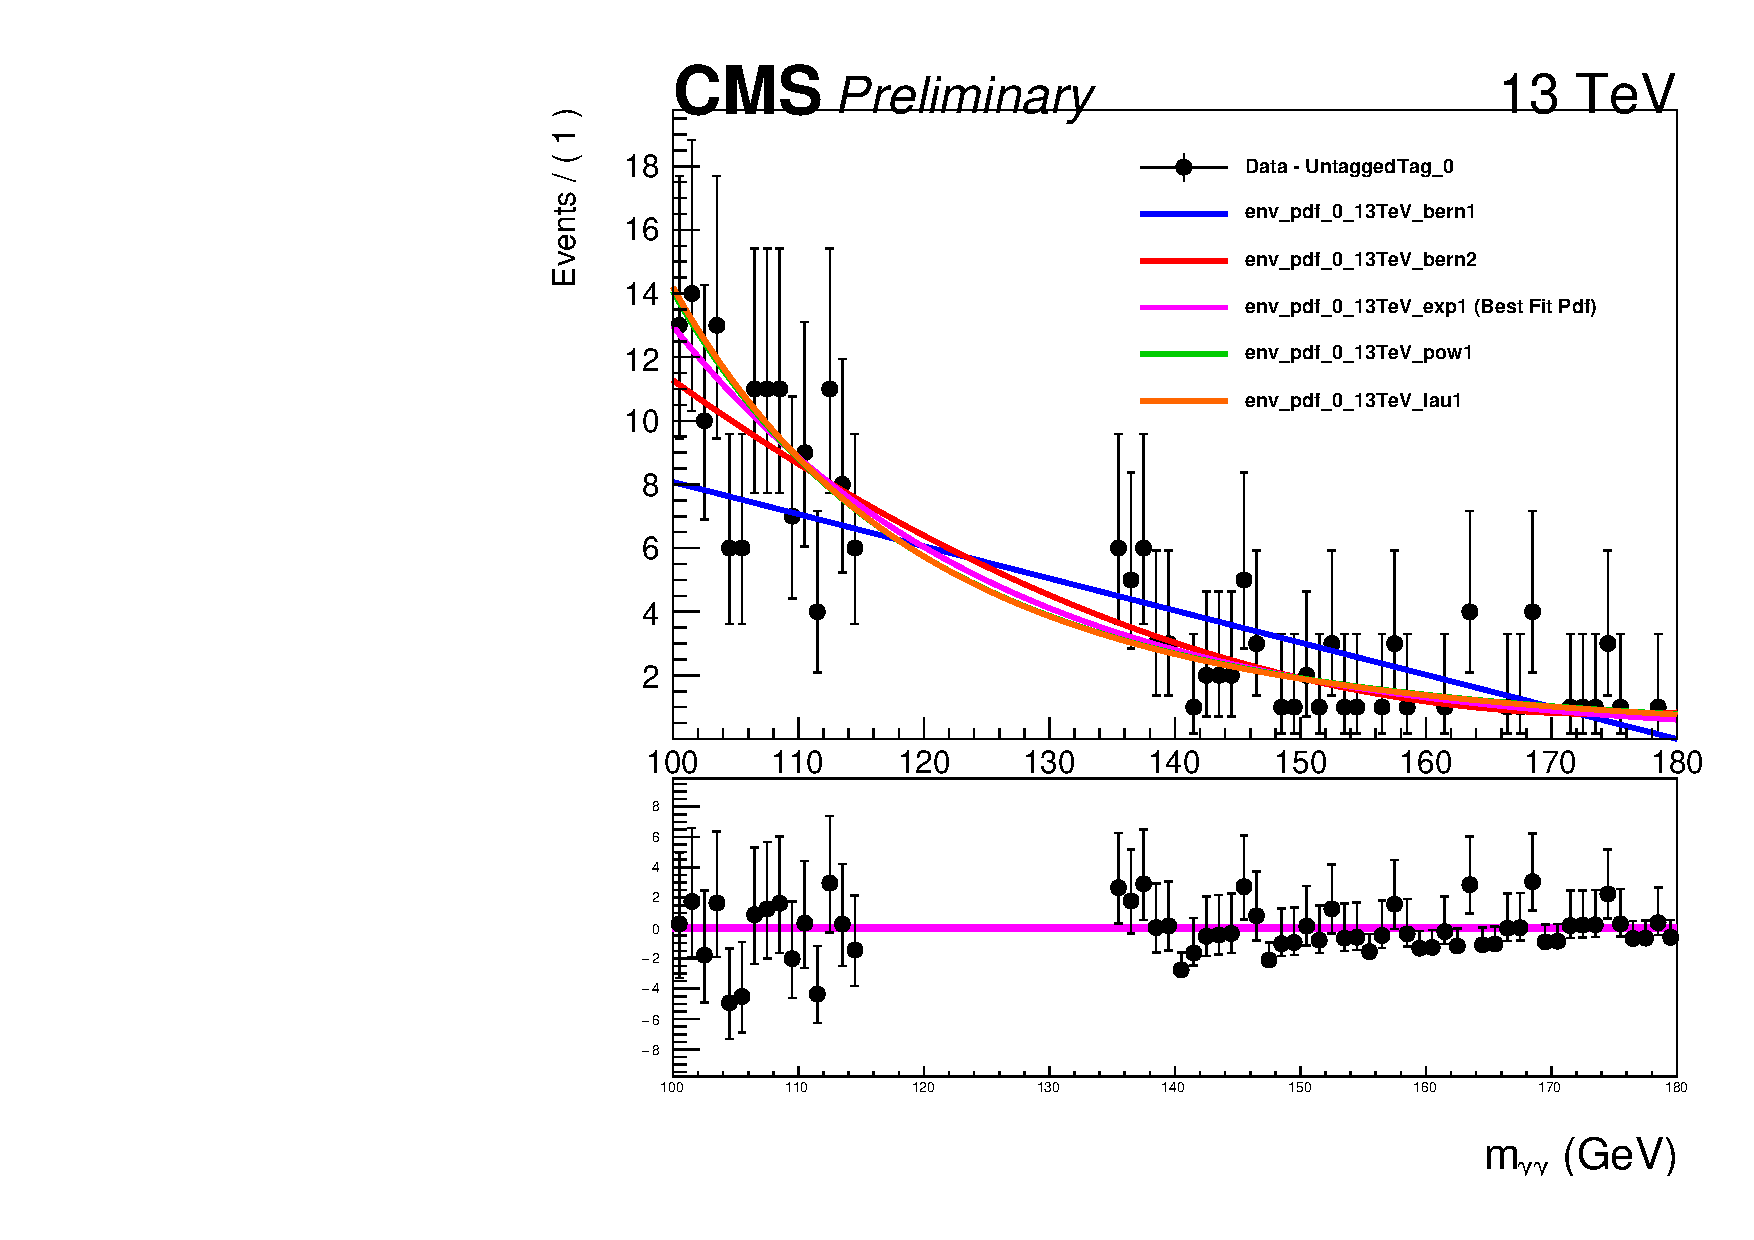
\includegraphics[width=0.48\textwidth]{modellingFigures/multipdf/multipdf_UntaggedTag_0.pdf}}
 \subfloat[UntaggedTag 1]{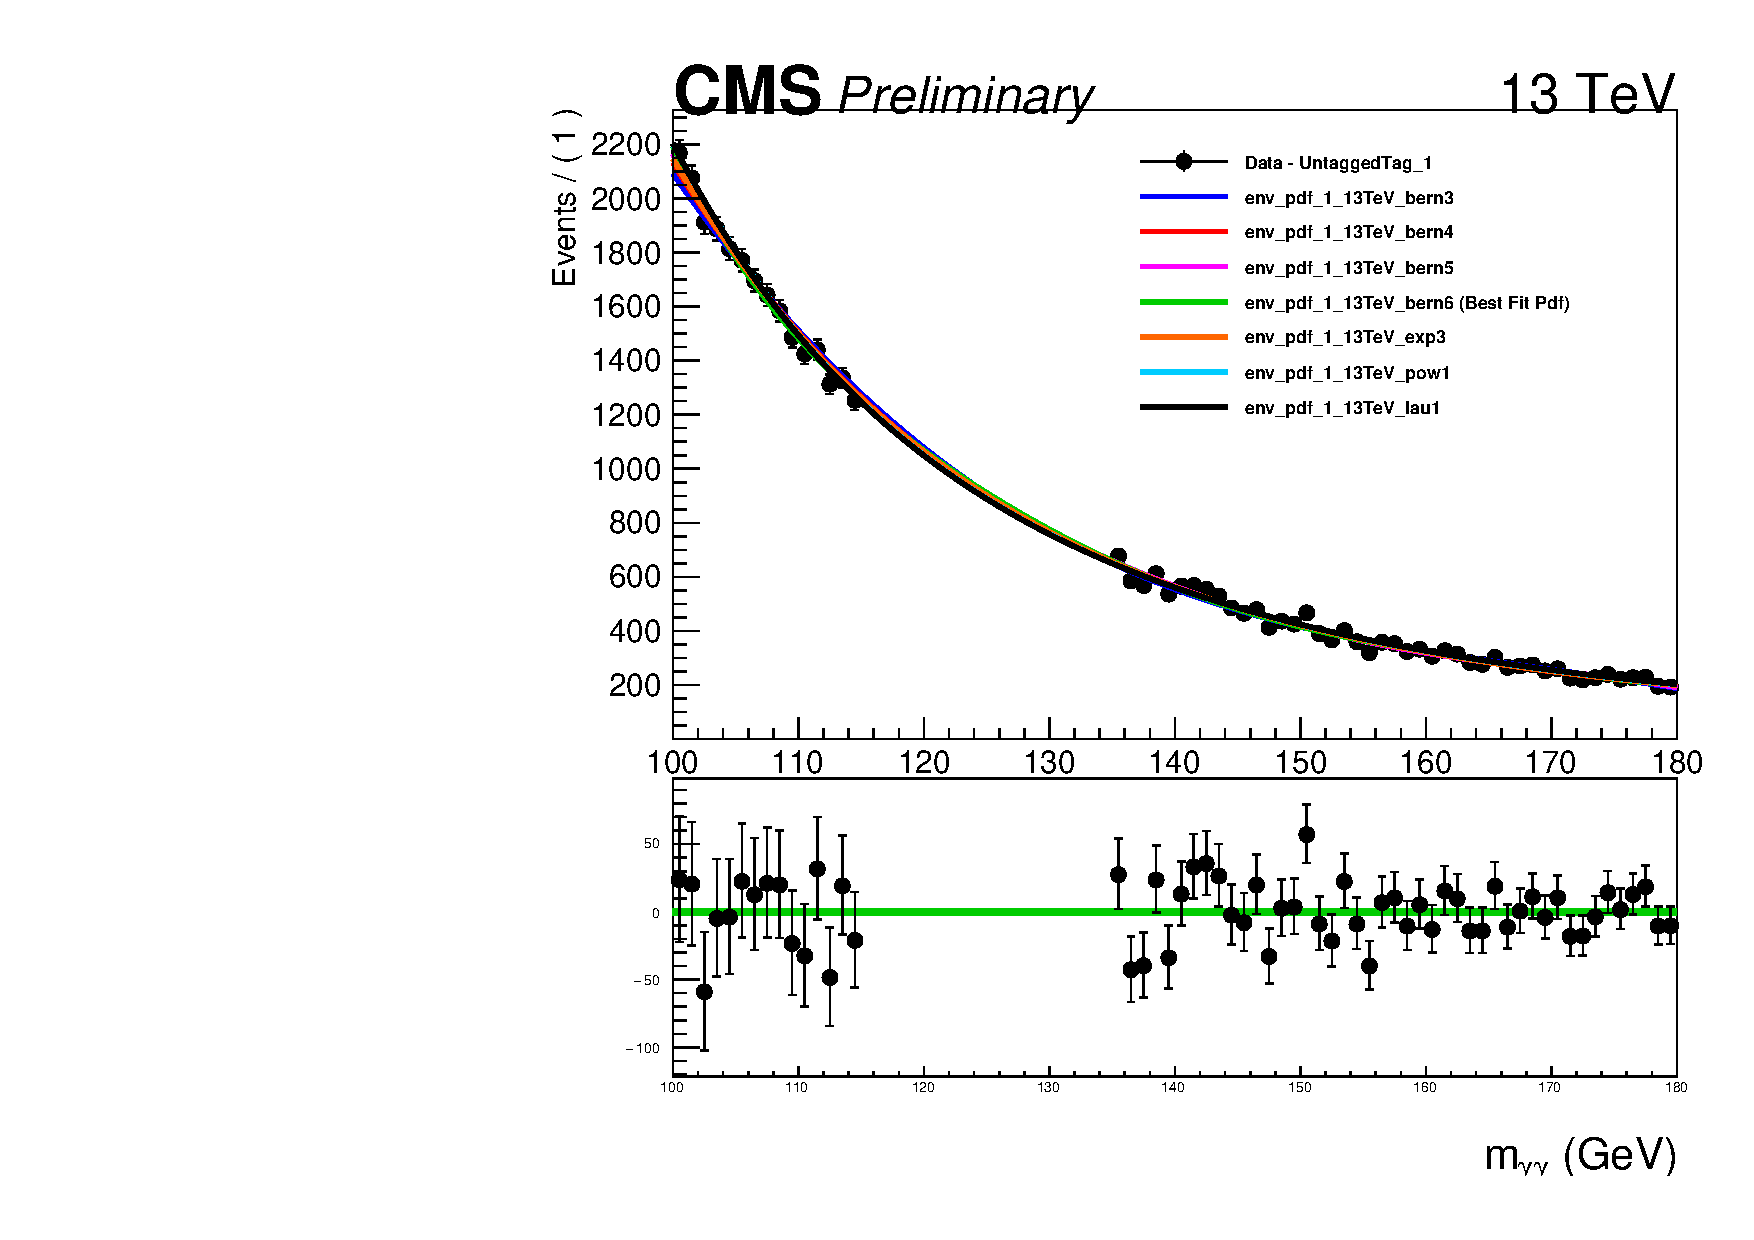
\includegraphics[width=0.48\textwidth]{modellingFigures/multipdf/multipdf_UntaggedTag_1.pdf}}\\
 \subfloat[UntaggedTag 2]{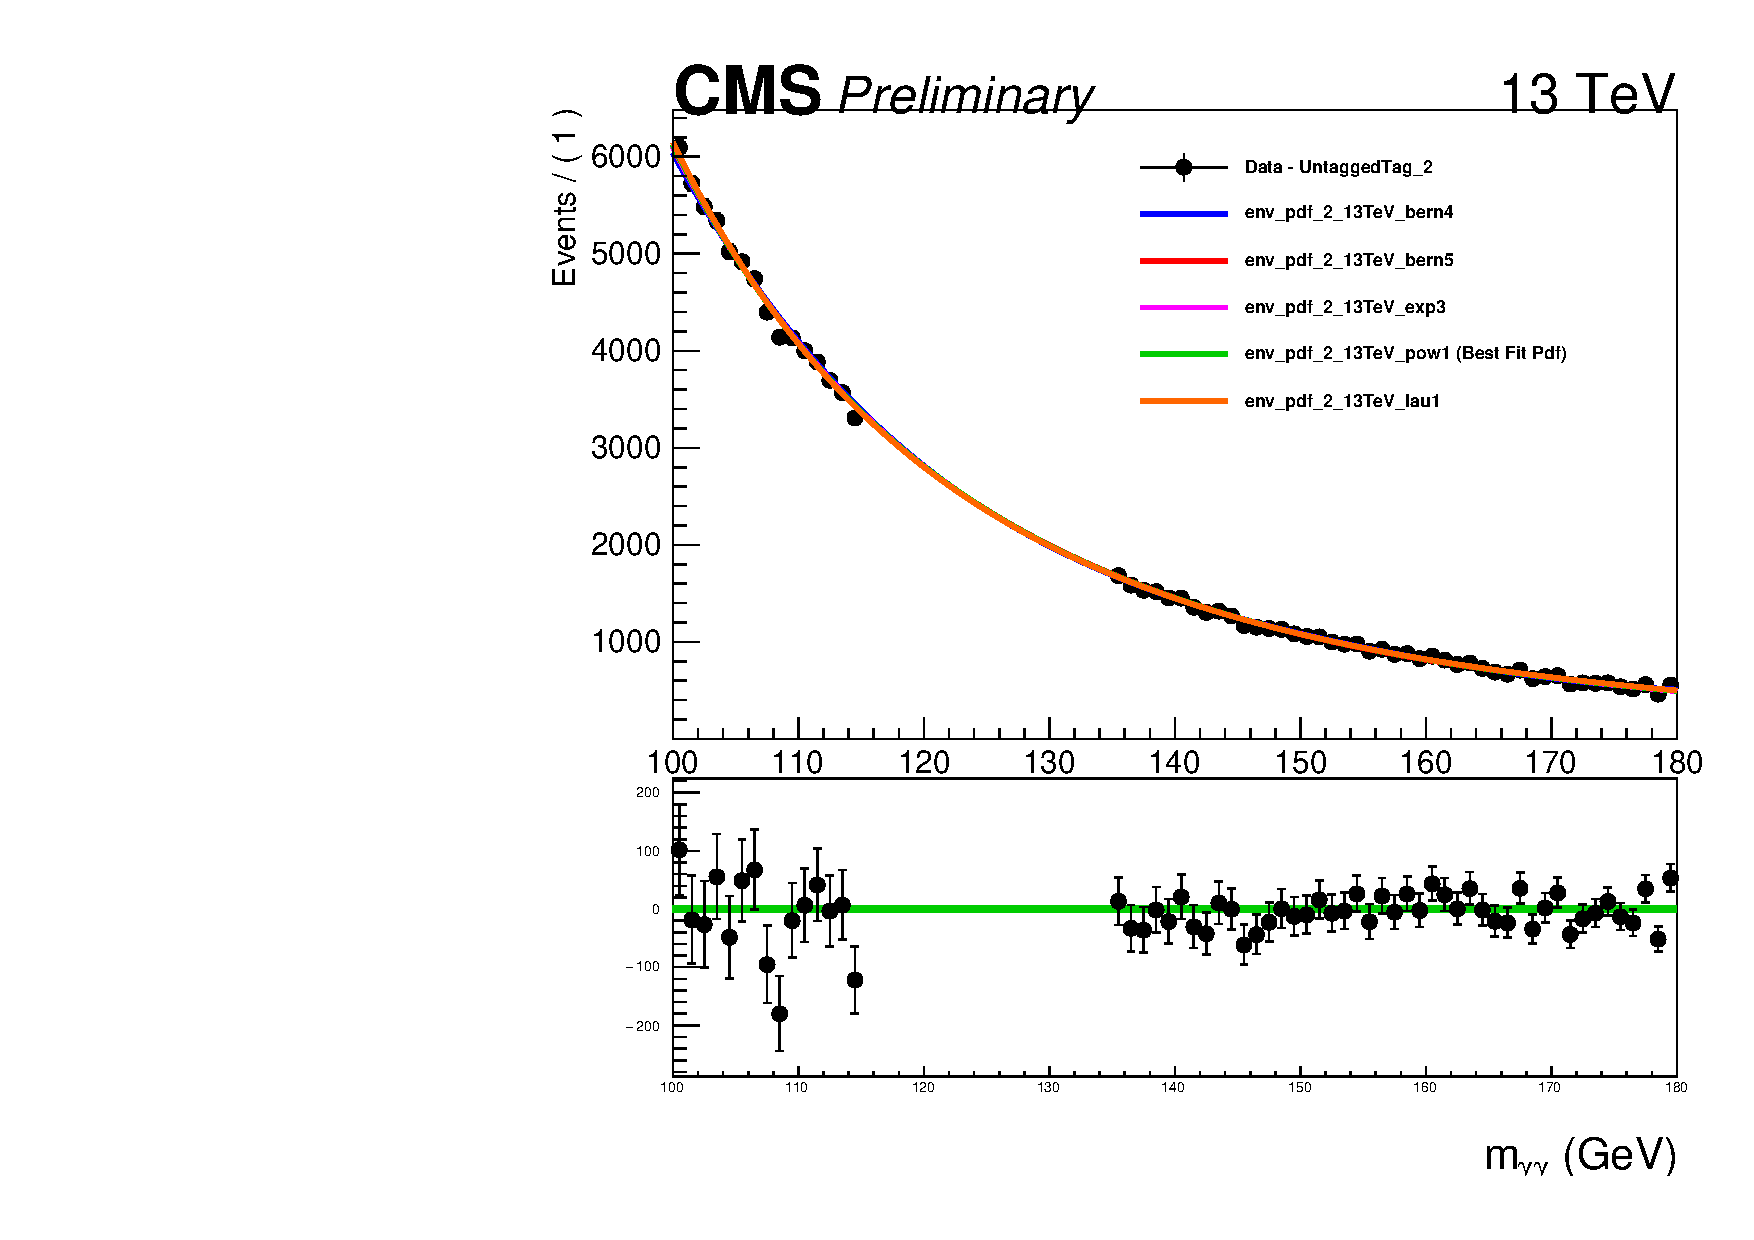
\includegraphics[width=0.48\textwidth]{modellingFigures/multipdf/multipdf_UntaggedTag_2.pdf}}
 \subfloat[UntaggedTag 3]{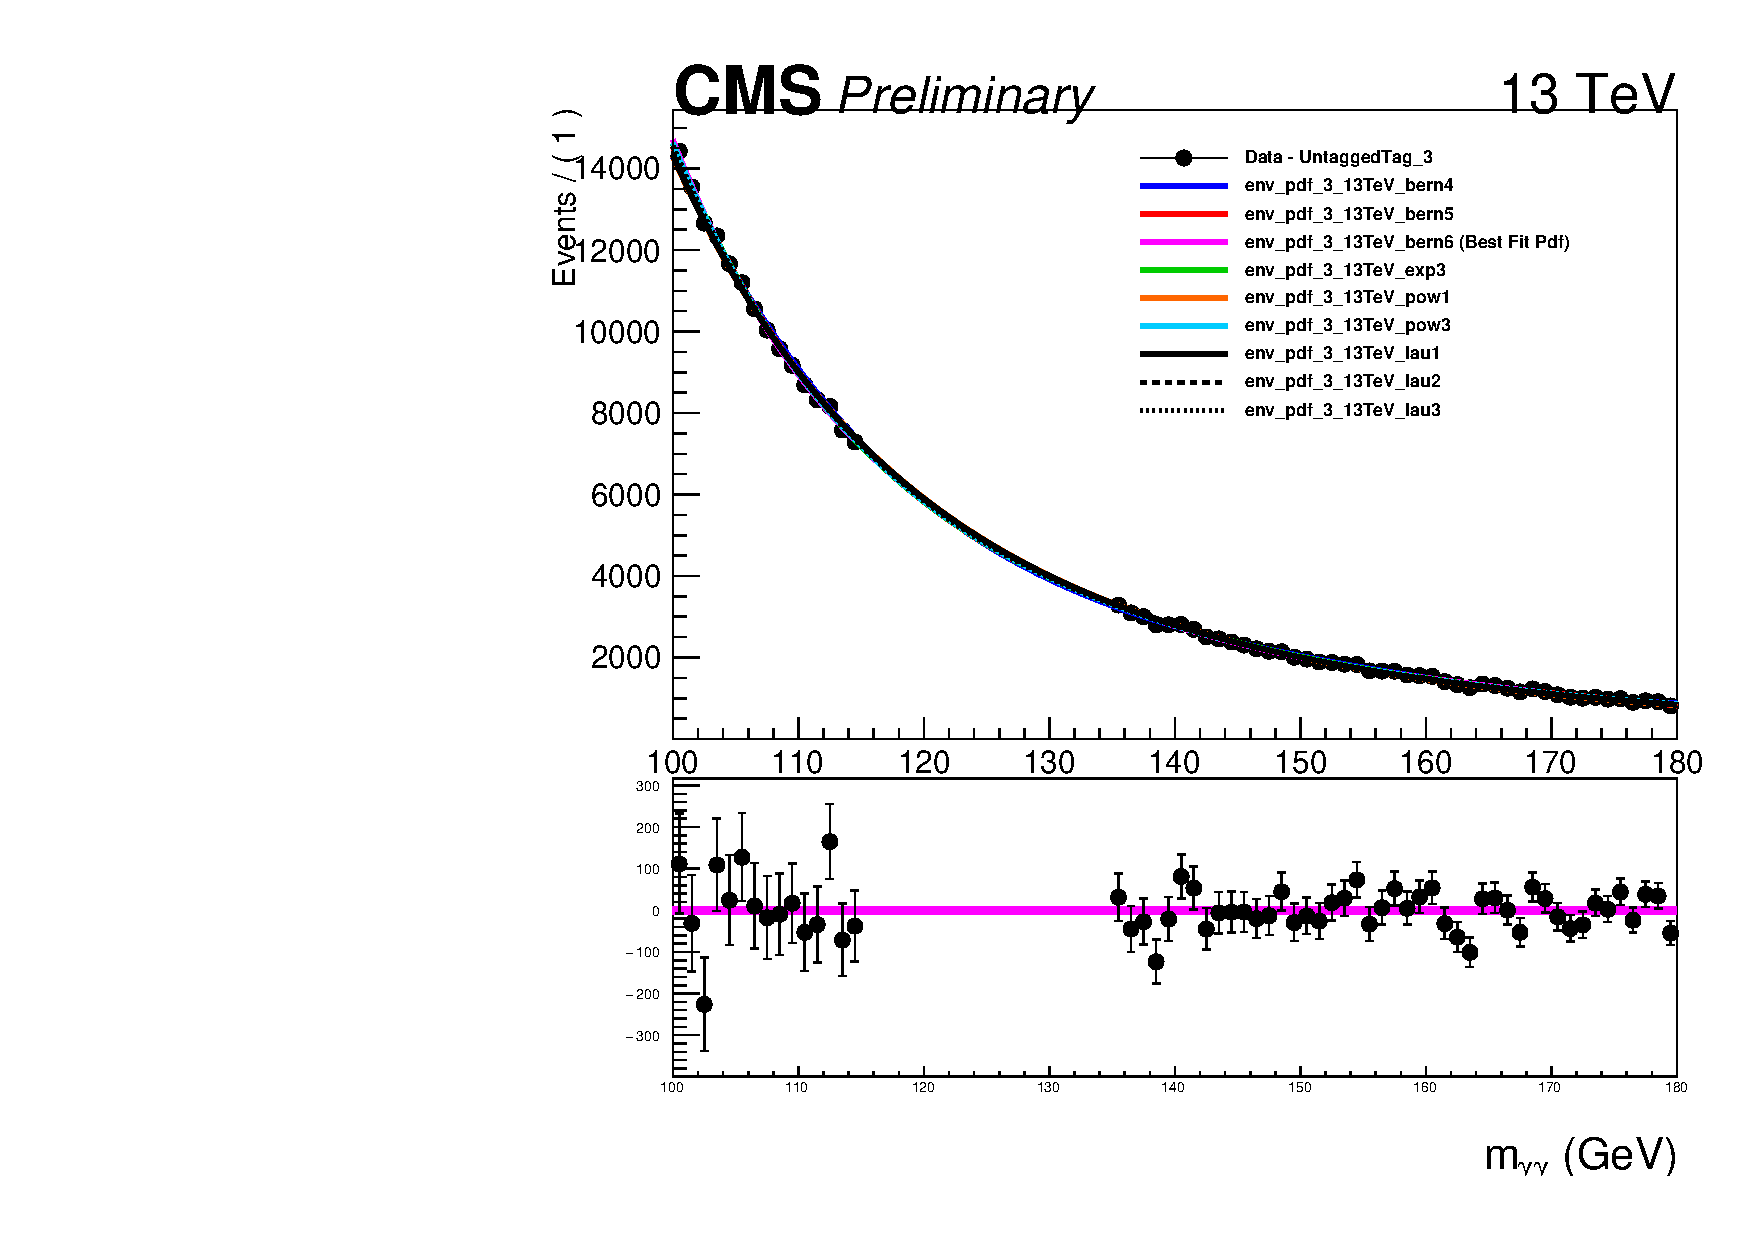
\includegraphics[width=0.48\textwidth]{modellingFigures/multipdf/multipdf_UntaggedTag_3.pdf}}\\
 \caption{The set of candidate functions chosen to parametrise the background using the discrete profiling method in the inclusive categories.}
 \label{fig:model_bkg)multipdf_inc}
 \end{center}
\end{figure}

\begin{figure}
 \begin{center}
 \subfloat[VBFTag 0]      {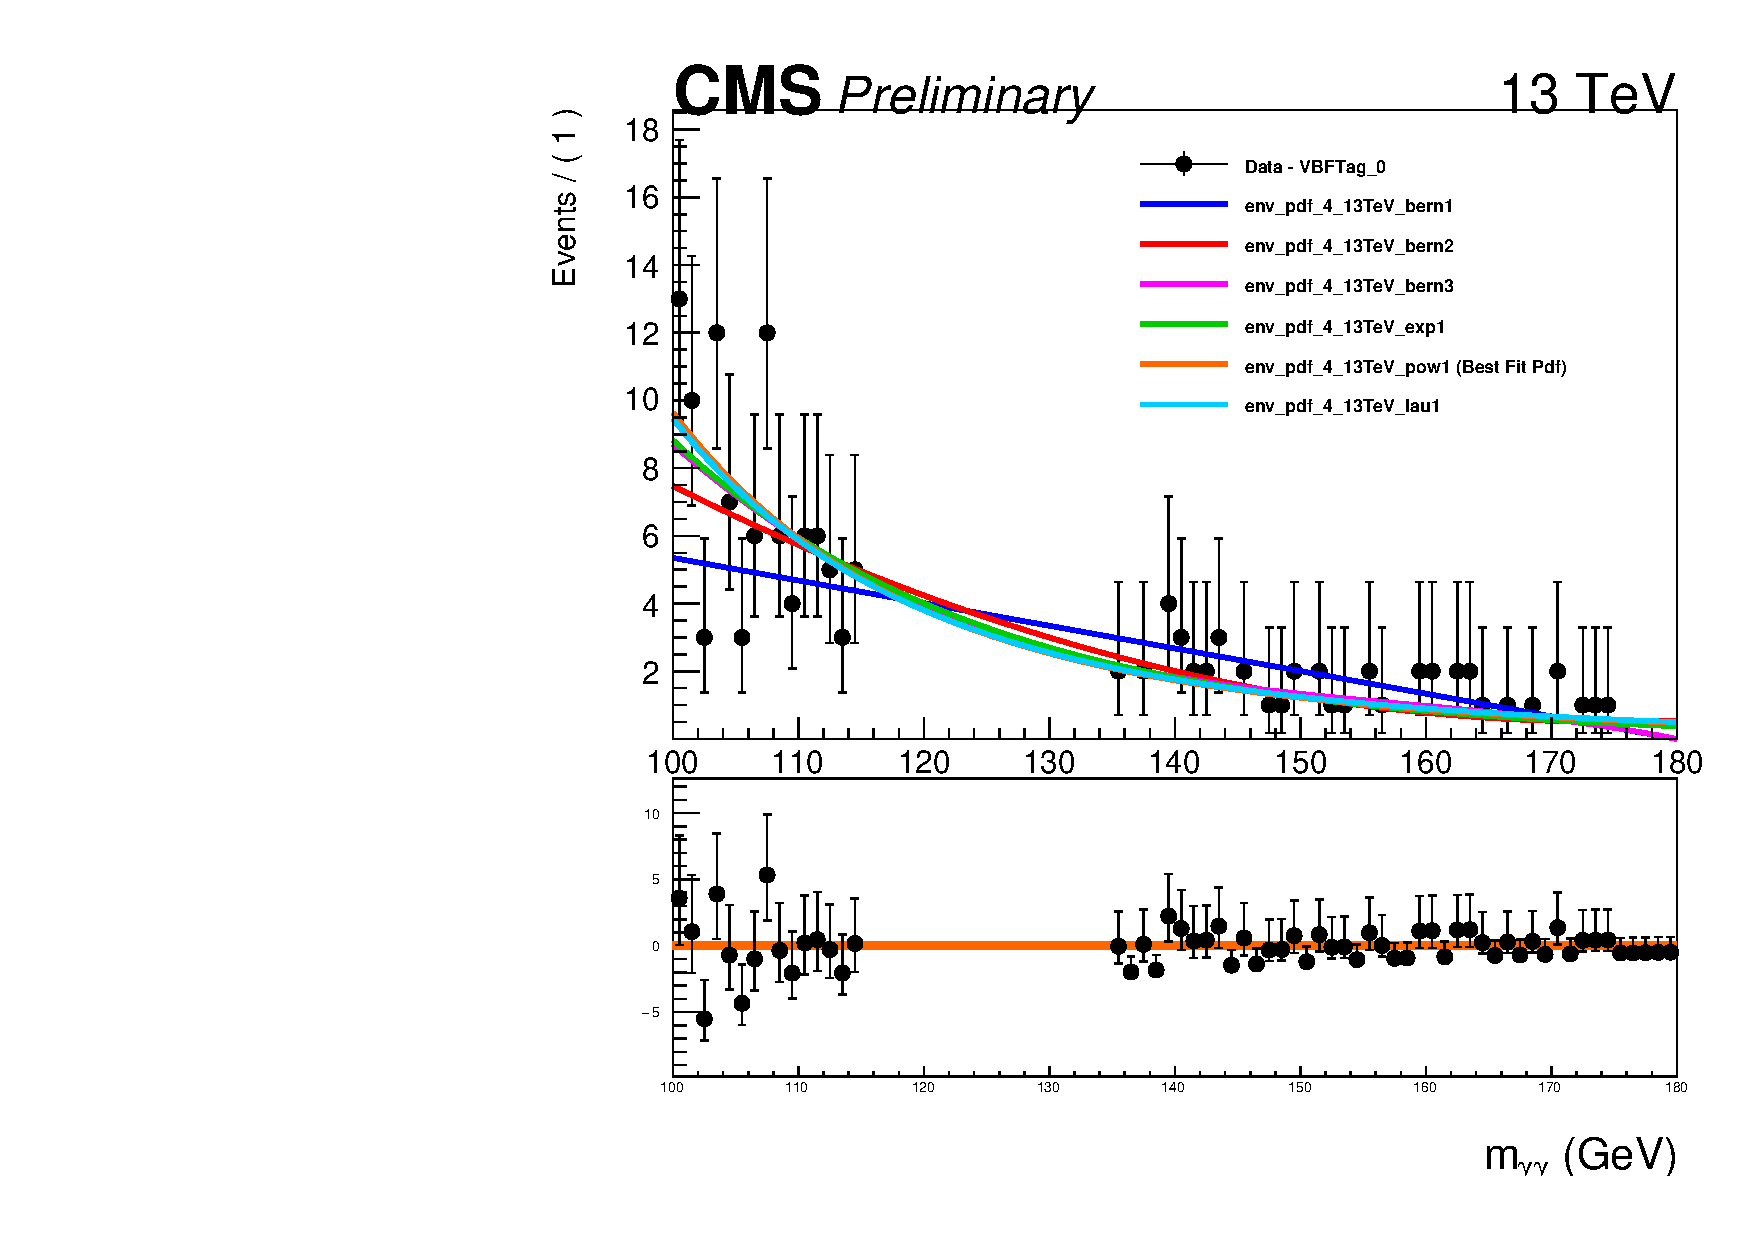
\includegraphics[width=0.48\textwidth]{modellingFigures/multipdf/multipdf_VBFTag_0.pdf}}
 \subfloat[VBFTag 1]      {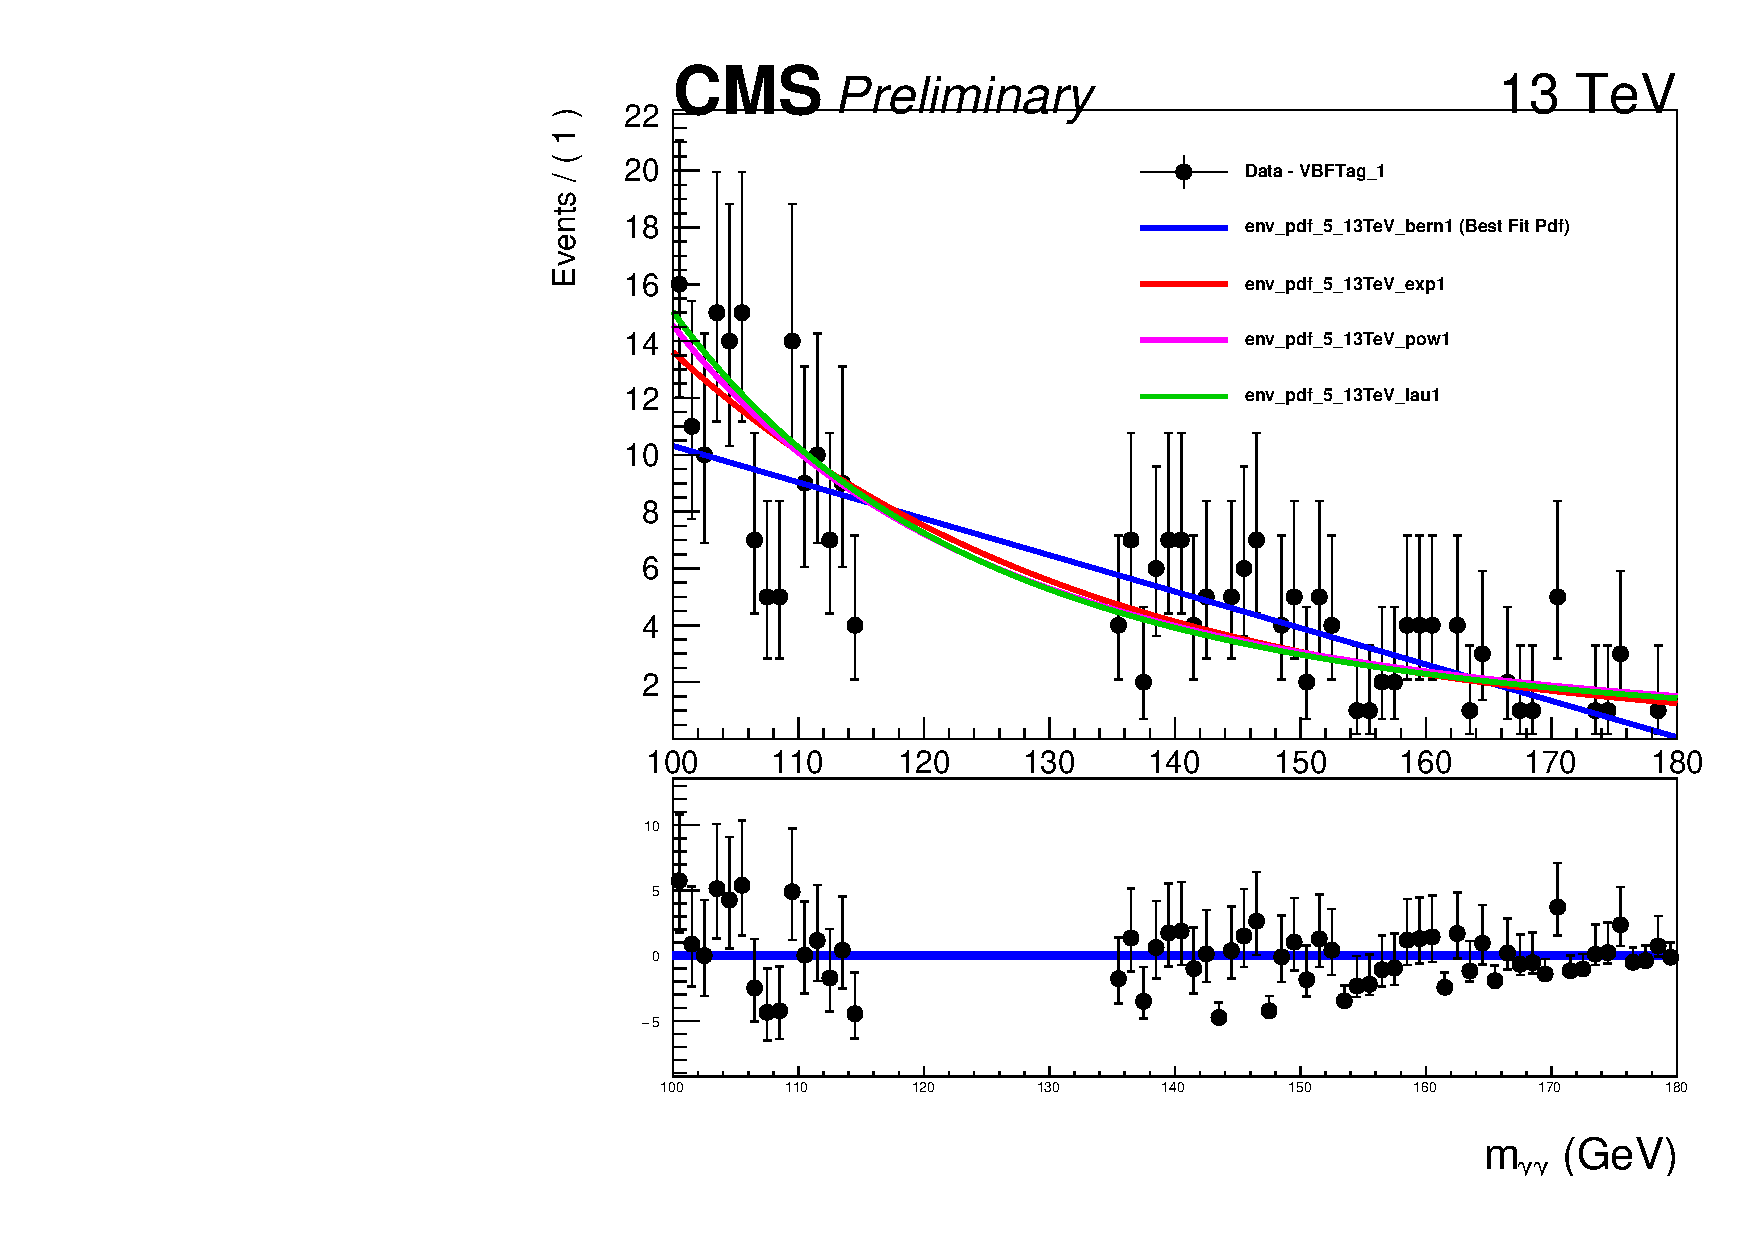
\includegraphics[width=0.48\textwidth]{modellingFigures/multipdf/multipdf_VBFTag_1.pdf}}\\
 \subfloat[TTHLeptonicTag]{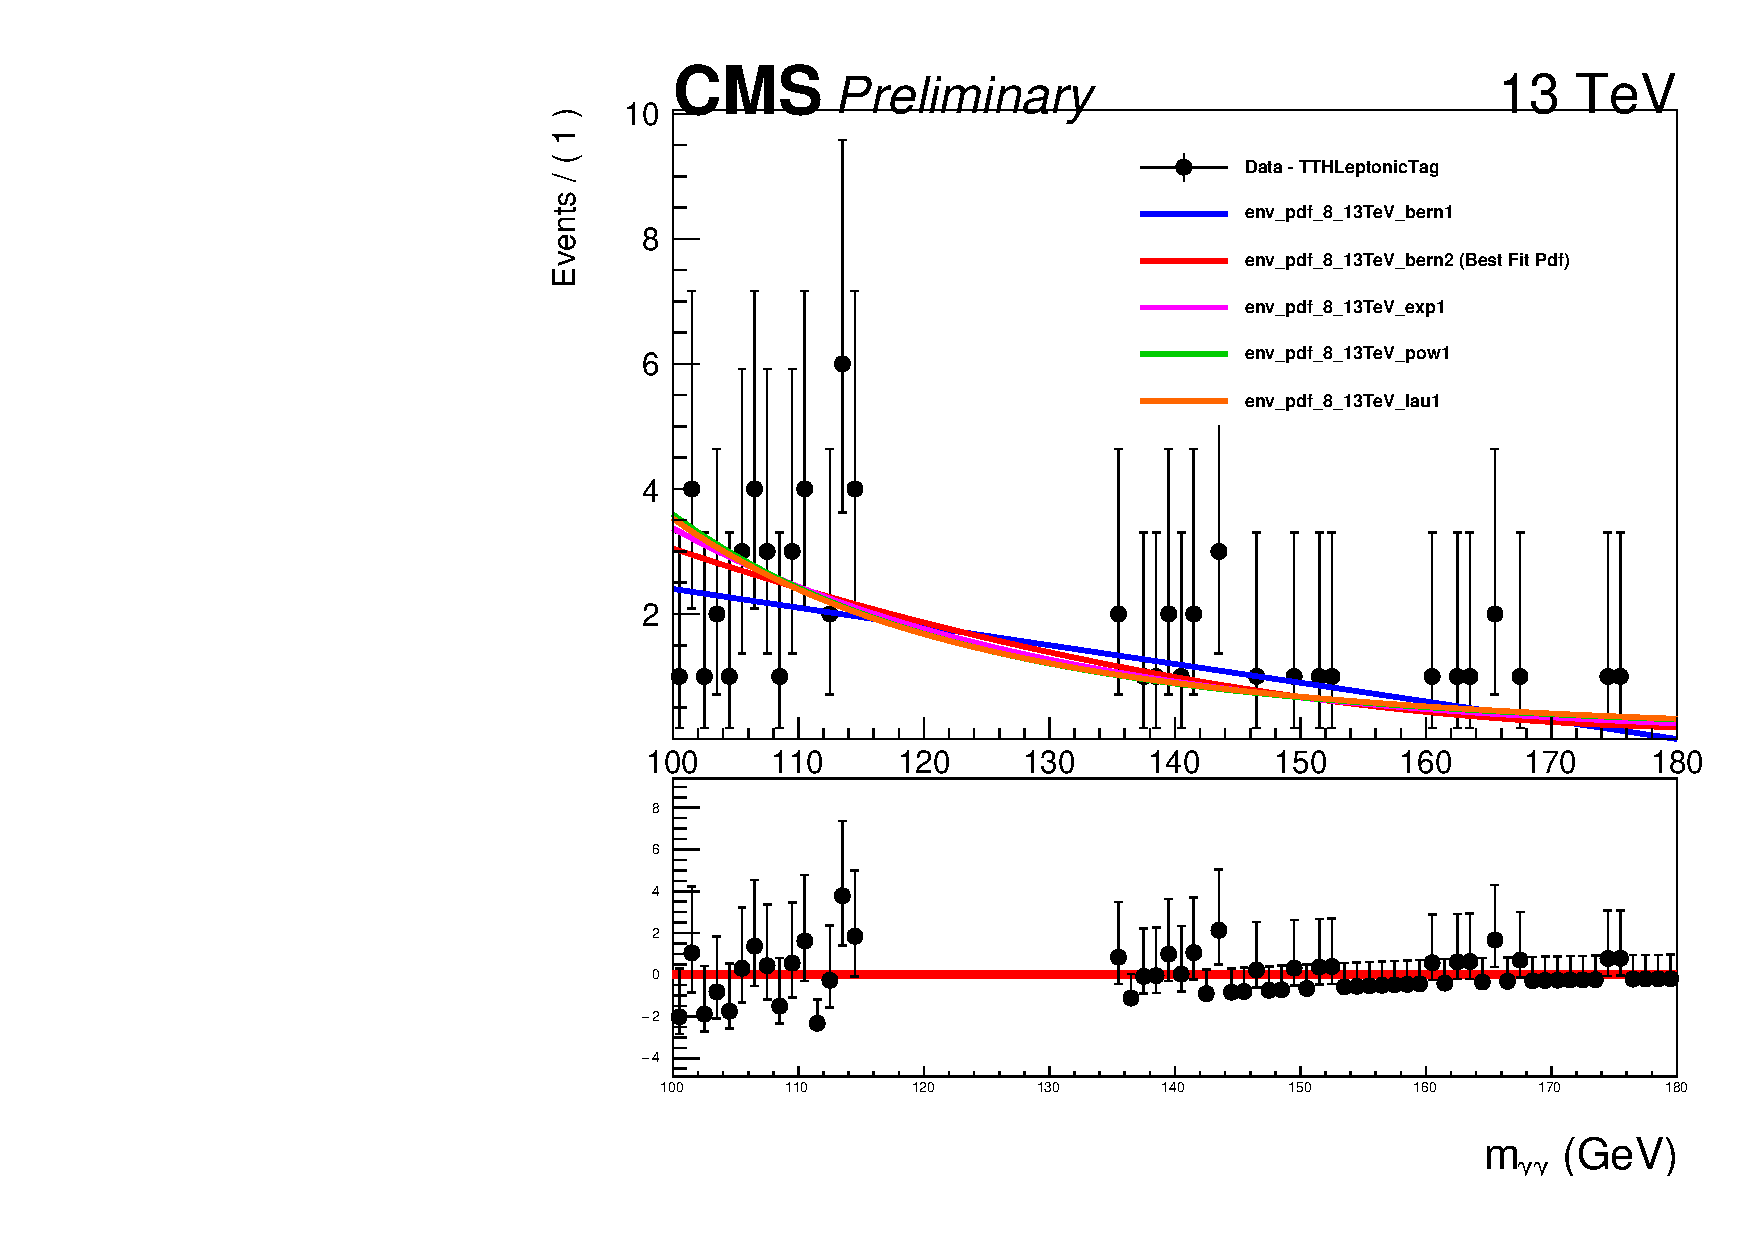
\includegraphics[width=0.48\textwidth]{modellingFigures/multipdf/multipdf_TTHLeptonicTag.pdf}}
 \subfloat[TTHHadronicTag]{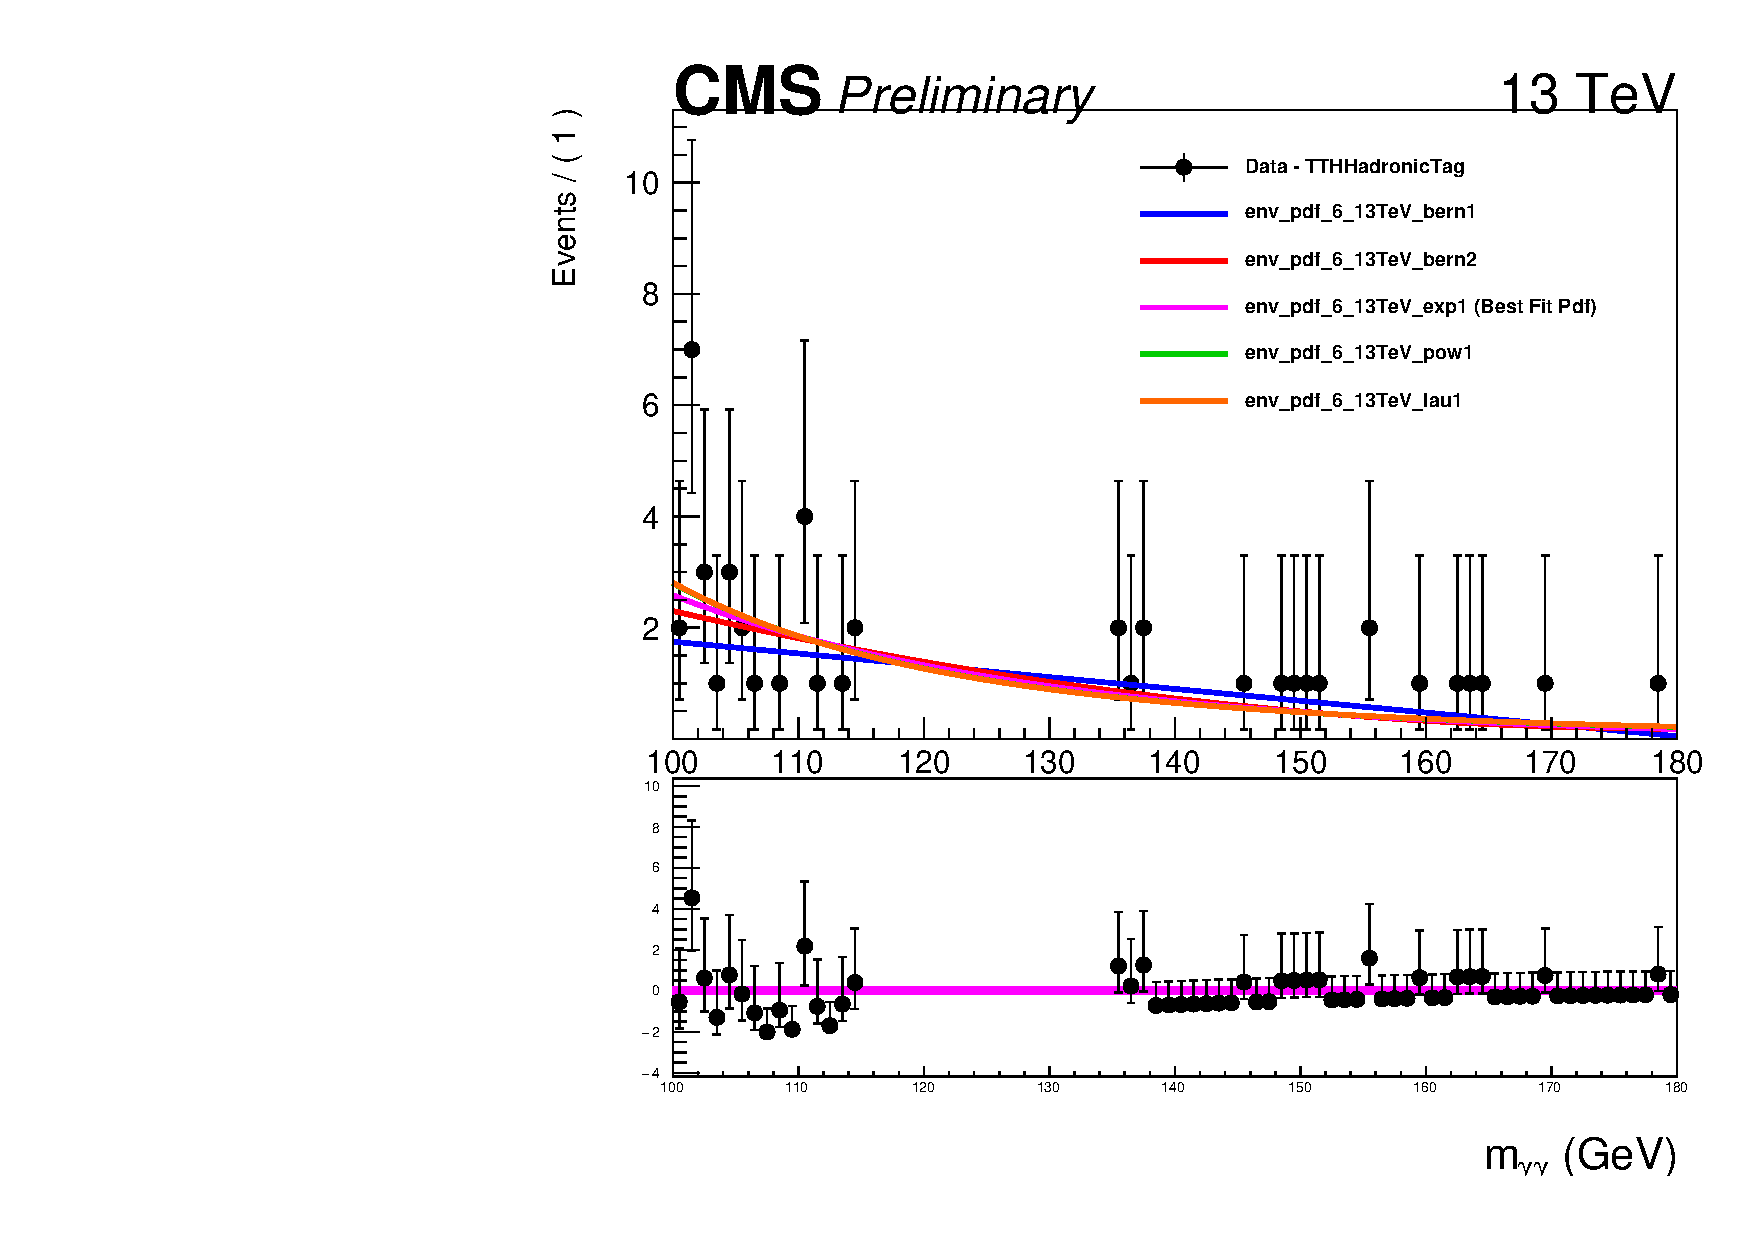
\includegraphics[width=0.48\textwidth]{modellingFigures/multipdf/multipdf_TTHHadronicTag.pdf}}\\
 \caption{The set of candidate functions chosen to parametrise the background using the discrete profiling method in the \VBFTag and \TTHTag categories.} 
 \label{fig:model:bkg_multipdf_exc}
 \end{center}
\end{figure}

The expected number of background events per $\GeV$ around $125\GeV$ is shown in \Table~\ref{tab:model:sig_bkg_yields} alongside the expecte number of signal events for each category, which is broken down by the contribution of each production mode. The \effSigma (the width of the smallest widnow containing $68.3\%$ of the distribution) and $\sigma_{HM}$ (the width of the distribution at half of the maximum value) of the signal model for each category are also shown. The expected number of background events is taken in a $\pm 1 \effSigma$ window around $125\GeV$ using the best-fit background function from the set of candidate functions in each category.

 \begin{table}
  \resizebox{\textwidth}{!}{
%%%%%%%%%%%%%%%%%%%%%%%%%%%%%%%%%%%%%%%%%%%%%%%%%%%%%%%
%\begin{tabular}{ |r | c | c | c  | c |  c |  c |  c |  c |  c | }
%\hline
%\multirow{2}{*}{Event Categories} &\multicolumn{8}{|l|}{SM 125GeV Higgs boson expected signal} & Average Bkg \\ \cline{2-9}
%  &  Total & ggh (\%) & vbf (\%) & wh (\%)  & zh (\%) & tth (\%)  &   $\sigma_{\text{eff}} $  & $\sigma_{\text{HM}} $ & (GeV$^{-1}$) \\
%  \hline
%  Untagged Tag 0 &    11.92  &  79.10  &  7.60  &  7.11  &  3.59  &  2.60 & 1.18 & 1.03 & 4.98 \\
%  Untagged Tag 1 &    128.78  &  85.98  &  7.38  &  3.70  &  2.12  &  0.82 & 1.35 & 1.20 & 199.14 \\
%  Untagged Tag 2 &    220.12  &  91.11  &  5.01  &  2.18  &  1.23  &  0.47 & 1.70 & 1.47 & 670.44 \\
%  Untagged Tag 3 &    258.50  &  92.35  &  4.23  &  1.89  &  1.06  &  0.47 & 2.44 & 2.17 & 1861.23 \\
%  VBF Tag 0 &    9.35  &  29.47  &  69.97  &  0.29  &  0.07  &  0.20 & 1.60 & 1.33 & 3.09 \\
%  VBF Tag 1 &    15.55  &  44.91  &  53.50  &  0.86  &  0.38  &  0.35 & 1.71 & 1.40 & 22.22 \\
%  TTH Hadronic Tag &    2.42  &  16.78  &  1.28  &  2.52  &  2.39  &  77.02 & 1.39 & 1.21 & 1.12 \\
%  TTH Leptonic Tag &    1.12  &  1.09  &  0.08  &  2.43  &  1.06  &  95.34 & 1.61 & 1.35 & 0.42 \\
%  Total &    647.77  &  87.93  &  7.29  &  2.40  &  1.35  &  1.03 & 1.88 & 1.52 & 2762.65 \\
%  \hline
%  \end{tabular}
  %%%%%%%%%%%%%%%%%%%%%%%%%%%%%%%%%%%%%%%%%%%%%%%%%%%%%%%
  %%%%%%%%%%%%%%%%%%%%%%%%%%%%%%%%%%%%%%%%%%%%%%%%%%%%%%%
  \begin{tabular}{ |r | c | c | c  | c |  c |  c |  c |  c |  c | }
  \hline
  \hline
  \hline
  \multirow{2}{*}{Event Categories} &\multicolumn{8}{|l|}{SM 125GeV Higgs boson expected signal} & Bkg Events\\ \cline{2-9}
    &  Total & ggh (\%) & vbf (\%) & wh (\%) & zh (\%) & tth (\%) &   $\sigma_{\text{eff}} $  & $\sigma_{\text{HM}} $ & in $ \pm \sigma_{eff}$  \\
    \hline
    \hline
    Untagged Tag 0 &    45.69  &  81.41  &  11.25  &  3.60  &  1.78  &  1.96 & 1.26 & 1.14 & 53.98 \\
    Untagged Tag 1 &    495.36  &  88.60  &  7.36  &  2.23  &  1.27  &  0.54 & 1.44 & 1.27 & 2630.66 \\
    Untagged Tag 2 &    661.79  &  91.23  &  5.50  &  1.83  &  1.04  &  0.40 & 1.96 & 1.68 & 9231.93 \\
    Untagged Tag 3 &    579.27  &  92.33  &  4.45  &  1.76  &  0.98  &  0.48 & 2.65 & 2.34 & 25503.31 \\
    VBF Tag 0 &    10.05  &  21.51  &  77.84  &  0.24  &  0.00  &  0.40 & 1.50 & 1.32 & 5.74 \\
    VBF Tag 1 &    12.31  &  36.48  &  62.50  &  0.38  &  0.16  &  0.48 & 1.62 & 1.33 & 23.05 \\
    VBF Tag 2 &    28.66  &  50.93  &  47.33  &  0.75  &  0.32  &  0.67 & 1.57 & 1.32 & 86.01 \\
    TTH Hadronic Tag &    5.38  &  11.36  &  0.81  &  0.73  &  2.12  &  84.98 & 1.42 & 1.29 & 6.64 \\
    TTH Leptonic Tag &    3.46  &  2.08  &  0.05  &  1.67  &  1.24  &  94.96 & 1.57 & 1.28 & 5.08 \\
    VH Met Tag &    10.84  &  46.42  &  3.36  &  19.47  &  21.73  &  9.02 & 1.78 & 1.51 & 72.96 \\
    VH LeptonicLoose Tag &    2.74  &  9.13  &  2.83  &  65.63  &  19.84  &  2.57 & 1.77 & 1.47 & 13.25 \\
    VH Hadronic Tag &    9.58  &  57.98  &  3.92  &  21.31  &  13.00  &  3.80 & 1.44 & 1.32 & 21.06 \\
    ZH Leptonic Tag &    0.52  &  0.00  &  0.00  &  0.00  &  97.37  &  2.63 & 1.60 & 1.33 & 0.39 \\
    WH Leptonic Tag &    3.59  &  1.24  &  0.66  &  87.53  &  4.77  &  5.80 & 1.63 & 1.35 & 6.71 \\
    Total &    1869.23  &  88.14  &  7.15  &  2.38  &  1.33  &  1.00 & 1.96 & 1.59 & 32056.29 \\
    \hline
    \hline
    \end{tabular}
    %%%%%%%%%%%%%%%%%%%%%%%%%%%%%%%%%%%%%%%%%%%%%%%%%%%%%%%

}
 \caption{ The expected number of signal and background events per category. The \effSigma of the signal model is also provided as an estimate of the $m_{\gamma\gamma}$ resolution in that category. The expected number of background events is quoted per \GeV in a $\pm 1 \effSigma$ window around 125 \GeV.}
 \label{tab:model:sig_bkg_yields}
\end{table}

\section{Sumamry of systematic uncertainties and their handling}

\subsection{theory uncertainties}
\subsection{experimental uncertainties}

